\documentclass[11pt,letterpaper]{article}
\usepackage[margin=0.85in]{geometry}
\usepackage[T1]{fontenc}
\usepackage{lmodern}
\usepackage{microtype}
\usepackage{amsmath,amssymb}
\usepackage{graphicx,booktabs,tabularx,array,multirow}
\usepackage{subcaption}
\usepackage{float}
\usepackage{placeins}
\usepackage{hyperref}
\usepackage[table]{xcolor}
\usepackage{longtable}
\usepackage{fancyhdr}
\usepackage{setspace}
\usepackage{enumitem}
\usepackage{tikz}
\usetikzlibrary{arrows.meta,positioning,calc,fit,backgrounds}
\usepackage{titlesec}
\definecolor{ink}{HTML}{22344A}
\definecolor{teal}{HTML}{137F80}
\definecolor{gold}{HTML}{D3943A}
\definecolor{mist}{HTML}{EFF5F6}
\definecolor{linegrey}{HTML}{8091A0}
\titleformat{\section}{\Large\bfseries\color{ink}}{\thesection}{0.7em}{}
\titleformat{\subsection}{\large\bfseries\color{teal}}{\thesubsection}{0.7em}{}
\tikzset{
 flow/.style={draw=teal!85!black,thick,fill=mist,rounded corners=3pt,align=center,inner sep=5pt,font=\scriptsize,text=ink},
 flowdark/.style={draw=ink,thick,fill=ink,rounded corners=3pt,align=center,inner sep=5pt,font=\scriptsize,text=white},
 flowgold/.style={draw=gold,thick,fill=gold!12,rounded corners=3pt,align=center,inner sep=5pt,font=\scriptsize,text=ink},
 flowsoft/.style={draw=linegrey,thick,fill=white,rounded corners=3pt,align=center,inner sep=5pt,font=\scriptsize,text=ink},
 arr/.style={-{Latex[length=2.3mm]},line width=0.75pt,draw=ink!85},
 conn/.style={line width=0.75pt,draw=ink!85},
 }
\newcommand{\tikzfit}[1]{\resizebox{\textwidth}{!}{\input{Diagrams/#1.tex}}}
\hypersetup{colorlinks=true,linkcolor=teal!80!black,urlcolor=teal!80!black,citecolor=teal!80!black}
\definecolor{reportblue}{HTML}{22344A}
\definecolor{reportgrey}{HTML}{627381}
\setstretch{1.07}
\setlength{\parskip}{0.36em}
\setlength{\parindent}{0pt}
\setlength{\tabcolsep}{5pt}
\renewcommand{\arraystretch}{1.12}
\setcounter{secnumdepth}{3}
\pagestyle{fancy}
\fancyhf{}
\fancyhead[L]{\small\color{reportgrey}Solar PV Prediction: P1--P5}
\fancyhead[R]{\small\color{reportgrey}ECE 579 | PV Machine Learning}
\fancyfoot[C]{\thepage}
\renewcommand{\headrulewidth}{0.3pt}
\newcommand{\fign}[3]{\begin{figure}[!htbp]\centering\includegraphics[width=0.91\textwidth]{#1}\caption{#2}\label{#3}\end{figure}}
\newcommand{\bestscore}[1]{\colorbox{teal!13}{\textcolor{teal!75!black}{\bfseries #1}}}
\newcommand{\smallnote}[1]{\vspace{2pt}{\footnotesize\color{reportgrey}#1}\vspace{5pt}}
% Highlight box used for key findings (no extra packages required).
\newcommand{\keybox}[2]{\par\smallskip\noindent\fcolorbox{teal!70!black}{mist}{%
  \begin{minipage}{\dimexpr\linewidth-2\fboxsep-2\fboxrule\relax}
  \textbf{\color{teal!75!black}#1}\par\vspace{2pt}#2
  \end{minipage}}\par\smallskip}

\begin{document}
\begin{titlepage}
\thispagestyle{empty}
\centering
\vspace*{0.30in}

\includegraphics[height=1.50in]{Assets/WPI_seal_from_uploaded_logo.png}\\[10pt]
{\large\bfseries Worcester Polytechnic Institute}\\[16pt]
{\color{teal}\rule{0.78\textwidth}{1.25pt}}\\[26pt]
{\Huge\bfseries\color{ink}Solar Photovoltaic Power\\[7pt] Prediction}\\[15pt]
{\Large\color{reportgrey}A Multi-Paradigm Machine Learning Study}\\[18pt]
{\color{teal}\rule{0.44\textwidth}{0.8pt}}\\[20pt]
\begin{minipage}{0.89\textwidth}\centering\large
Supervised Classification \textbullet\ Supervised Regression\\[7pt]
Dimensionality Reduction \textbullet\ Semi-Supervised Learning\\[7pt]
Cross-City Transfer Learning
\end{minipage}\\[28pt]
{\large\bfseries ECE 579: Machine Learning for Engineering Applications}\\[12pt]
{\normalsize\textbf{Instructor:} Prof.\ Ziming Zhang}\\[12pt]
{\large\textbf{Student:} Albert Shaju}\\[5pt]
{\normalsize Department of Electrical and Computer Engineering}\\[13pt]
{\normalsize Machine Learning Course Project Report}\\[6pt]
{\normalsize November 2026}\\[18pt]
{\small\textbf{Video presentation:} \href{https://drive.google.com/file/d/1yEQ6FFIMTAmYXIgzWIxX5eqDjJoTPSaY/view?usp=sharing}{Google Drive link}}\\[4pt]
{\small\textbf{Code and results:} \url{https://github.com/myProjects400/ECE579-PV-ML-Project}}
\vfill
\end{titlepage}

% =================================================================
\section*{Abstract}
\addcontentsline{toc}{section}{Abstract}
Photovoltaic (PV) generation is intermittent because it follows irradiance, clouds and
temperature, and grid operators therefore need reliable short-horizon estimates of array
output. Using the five-city NSRDB/PV workbook supplied for the course (Davis, Huron,
Santa Barbara, La Jolla and Amherst; three- and six-year histories), this project studies
five connected learning paradigms: supervised classification (P1), supervised regression (P2),
unsupervised dimensionality reduction followed by prediction (P3), semi-supervised
classification (P4) and cross-city transfer learning (P5). Every experiment uses chronological
train/test splits, preprocessing fitted on training data only, and three fixed seeds
(42, 123, 2026); for each problem, linear, kernel, tree-ensemble and neural models are compared.

Same-city sky-condition classification reaches $99.15\%$ balanced accuracy (Davis, XGBoost),
while the generation-regime task drops from $96.35\%$ in Davis to $75.90\%$ in Amherst, where the
\emph{Medium} regime is recognised only $60.8\%$ of the time. Same-city power regression reaches
$11.85$\,kW RMSE ($4.72\%$ nRMSE) in Davis, but Davis-trained models applied unchanged to other
cities exceed $100\%$ nRMSE, consistent with a substantial site-level output-scale
mismatch: Davis produces about $3.3$--$3.5\times$ the average power of the tested targets. Compressing the inputs to 2, 5 or 10 unsupervised components never beat the
full-feature model, and pseudo-labeling or autoencoder SSL changed balanced accuracy by less than
$0.2$ percentage points at $10\%$ labels for the best classifier. The strongest single result is in
transfer learning: with only ten labeled Amherst observations, jointly calibrated source--target
pooling cuts held-out RMSE from $75.82$\,kW (zero-shot) to $23.22$\,kW, a $69\%$ reduction, and
beats the matched ten-label target-only model by $2.97$\,kW. Across all five problems, the
recurring lesson is that \emph{site-specific output scale}, not model family, dominates the error
budget, and that well-tuned tree ensembles are as good as or better than neural networks on
this tabular data.

\smallskip
\noindent\textbf{Keywords:} photovoltaic forecasting; balanced accuracy; nRMSE; PCA; autoencoder;
pseudo-labeling; domain shift; few-shot transfer.

\clearpage
\tableofcontents
\clearpage

\section*{List of Abbreviations}
\addcontentsline{toc}{section}{List of Abbreviations}
\noindent\textcolor{reportgrey}{Key terminology used throughout the photovoltaic machine-learning experiments.}
\vspace{0.8em}

\begingroup
\small
\renewcommand{\arraystretch}{1.05}
\setlength{\tabcolsep}{4pt}
\renewcommand{\tabularxcolumn}[1]{m{#1}}
\begin{tabularx}{\textwidth}{@{}>{\bfseries\color{ink}}m{0.19\textwidth}X@{}}
\toprule
Abbreviation & Full term / meaning \\
\midrule
AE & Autoencoder \\
AI & Artificial Intelligence \\
AUC & Area Under the Curve (label-efficiency curve) \\
BA & Balanced Accuracy (mean per-class recall) \\
DHI & Diffuse Horizontal Irradiance \\
DNI & Direct Normal Irradiance \\
GHI & Global Horizontal Irradiance \\
ID & In-distribution (same-city) evaluation \\
KPCA & Kernel Principal Component Analysis \\
LSTM & Long Short-Term Memory network \\
MAE & Mean Absolute Error \\
MLP & Multilayer Perceptron \\
MSE & Mean Squared Error \\
nRMSE & Range-normalized Root Mean Squared Error \\
NSRDB & National Solar Radiation Database \\
P1--P5 & Project Problems 1 through 5 \\
PCA & Principal Component Analysis \\
PV & Photovoltaic \\
RBF & Radial Basis Function (kernel) \\
RF & Random Forest \\
RMSE & Root Mean Squared Error \\
SD & Standard Deviation (across three seeds) \\
SSL & Semi-Supervised Learning \\
SVM & Support Vector Machine \\
SVR & Support Vector Regression \\
t-SNE & t-distributed Stochastic Neighbor Embedding \\
UMAP & Uniform Manifold Approximation and Projection \\
XGBoost & Extreme Gradient Boosting \\
\bottomrule
\end{tabularx}
\endgroup
\clearpage

% =================================================================
\section{Introduction}
\subsection{Motivation}
Photovoltaic arrays are one of the fastest-growing sources of electricity, but unlike
dispatchable plants their output follows the weather: irradiance, cloud cover, temperature and
wind change from minute to minute. Very-short-term estimates of array output let grid operators
balance load, smooth ramps, limit voltage flicker and schedule storage.
Building such estimators is not a single learning problem. Labels can be discrete (sky regime)
or continuous (power); sensors fail, so labels may be scarce; and a model trained at one site is
often needed at another site with different weather and a different installed capacity.

\subsection{Scope and contributions}
This report studies five connected problems on the same data foundation. P1 classifies sky
condition and generation regime; P2 regresses Output Power in same-city, cross-city, sequential
and history-length settings; P3 asks whether unsupervised compression to $d\in\{2,5,10\}$
components preserves predictive information; P4 measures the value of unlabeled data at
$10/30/50\%$ label budgets; and P5 transfers knowledge from data-rich Davis to label-scarce
Amherst. The main contributions are:
\begin{itemize}[leftmargin=1.5em,itemsep=2pt]
\item a leakage-safe common protocol (chronological split, train-only preprocessing, three seeds)
applied identically to every method within each comparison;
\item for every problem, a comparison of at least four classical models and at least one PyTorch
neural model (MLP, LSTM or autoencoder), reported as mean $\pm$ SD with all models shown;
\item matched-baseline analyses for SSL (same labeled subset) and transfer learning (same $k$
target labels), so that reported gains isolate the effect of unlabeled data or source knowledge;
\item a cross-problem analysis that links the P1 Amherst generation difficulty, the P2 zero-shot
failure and the P5 calibration success to a single cause.
\end{itemize}

Figure~\ref{fig:overall} maps the experiments: the nine input sheets first undergo a chronological
split and training-only transformations, after which the five paradigms address different
prediction and data-availability questions. The branches reunite only at held-out evaluation; no
single model is shared across all tasks.

\begin{figure}[!htbp]\centering
\tikzfit{overall_workflow}
\caption{Project-wide analysis pipeline. Each problem reuses the same PV data foundation but applies task-specific preprocessing, evaluation protocols, and models.}\label{fig:overall}
\end{figure}

\paragraph{Study questions.} (i) Which models perform best in supervised same-city settings?
(ii) How does accuracy change across cities and time-series protocols? (iii) What is
the cost of reducing feature dimensions? (iv) When does unlabeled training data improve prediction?
(v) Can source-city information reduce the number of labels needed in a target city?

\subsection{Summary of best results}
Table~\ref{tab:headline} collects the best observed held-out result of every problem in one
place; each entry is a three-seed mean and is traced to its full table in the corresponding
section.

\begin{table}[!htbp]\centering\footnotesize
\caption{Headline results (held-out test, mean over three seeds). BA = balanced accuracy; RMSE in kW. Each row names the best observed model; full comparisons appear in Sections~\ref{sec:p1}--\ref{sec:p5}.}\label{tab:headline}
\setlength{\tabcolsep}{4pt}
\renewcommand{\arraystretch}{1.18}
\begin{tabularx}{\textwidth}{@{}l>{\raggedright\arraybackslash}p{4.3cm}>{\raggedright\arraybackslash}X>{\raggedright\arraybackslash}p{3.6cm}@{}}\toprule
\textbf{Problem} & \textbf{Setting} & \textbf{Best result (model)} & \textbf{Reference point}\\\midrule
P1 & Sky condition, Davis / Amherst & \bestscore{99.15\%} BA (XGBoost) / 98.82\% (XGBoost) & 3 classes; chance $=33.3\%$\\
P1 & Generation regime, Davis / Amherst & 96.35\% BA (XGBoost) / 75.90\% (RF) & Amherst \emph{Medium} recall 60.8\%\\
P2 & Same-city, Davis / Amherst & \bestscore{11.85 kW} (4.72\%) XGBoost/MLP / 19.96 kW (15.69\%) MLP & Ridge: 13.82 / 20.72 kW\\
P2 & Sequential $K{=}12$, Davis / Amherst & 13.30 kW (5.29\%) / 15.96 kW (12.54\%), RF & LSTM: 14.64 / 16.55 kW\\
P2 & Zero-shot Davis$\to$Huron / SB / LJ & 114.61 / 102.96 / 77.27 kW, RBF SVR & $>100\%$ nRMSE everywhere\\
P2 & 3-yr vs 6-yr history (best nRMSE) & Davis 4.72$\to$4.58\%, Huron 4.49$\to$4.47\%, LJ 8.16$\to$7.87\% & SB worsens 12.09$\to$12.27\%\\
P3 & Closest reduced vs raw & Amherst gen.: KPCA-10 75.56\% vs 76.06\% & Raw features win all 8 cases\\
P4 & 10\% labels, best SSL vs best supervised & $+0.08$ to $+0.16$ pp (3 of 4 tasks) & Largest matched gain $+5.59$ pp (MLP)\\
P5 & Davis$\to$Amherst, $k=10$ labels & \bestscore{23.22 kW} joint pooling (Ridge) & Zero-shot 75.82; target-only 26.19\\
\bottomrule\end{tabularx}
\end{table}

\keybox{Single most interesting finding}{Davis-trained regressors that achieve $\approx 5\%$
nRMSE at home exceed $100\%$ nRMSE in every other city, because the source array produces
$3.3$--$3.5\times$ more power (Table~\ref{tab:citypower}). Yet the same Davis knowledge becomes
useful again after a cheap correction: ten labeled Amherst observations are enough to calibrate
and pool the source data, lowering RMSE by $69\%$ relative to zero-shot and by $11\%$ relative to a
ten-label target-only model. The weather-to-power \emph{shape} transfers between cities; the
absolute \emph{scale} does not.}

% =================================================================
\section{Data and Experimental Design}
\subsection{Data source}
The workbook \emph{Further Consolidated Data, HnL.xlsx} contains nine sheets of half-hourly
irradiance, meteorology and PV output recorded between about 10:00 and 14:30 local solar time,
the productive mid-day window. Table~\ref{tab:sheets} lists the sheets and
how each is used here.

\begin{table}[!htbp]\centering\footnotesize
\caption{Workbook sheets and their role in this project. Maximum Output Power ranges from roughly 72\,kW (La Jolla) to 263\,kW (Davis) according to the course specification.}\label{tab:sheets}
\setlength{\tabcolsep}{5pt}
\begin{tabularx}{\textwidth}{@{}llX@{}}\toprule
\textbf{City} & \textbf{Sheets (years)} & \textbf{Used in}\\\midrule
Davis, CA & 2011--2016 and 2014--2016 & P1--P4 same-city; P2 zero-shot source; P2 history ablation; P5 source\\
Amherst, MA & 2018--2020 (three years only) & P1--P4 same-city; P5 label-scarce target\\
Huron, SD & 2011--2016 and 2014--2016 & P2 zero-shot target; P2 history ablation\\
Santa Barbara, CA & 2011--2016 and 2014--2016 & P2 zero-shot target; P2 history ablation\\
La Jolla, CA & 2011--2016 and 2014--2016 & P2 zero-shot target; P2 history ablation\\
\bottomrule\end{tabularx}
\end{table}

Each sheet has 22 columns, grouped in Table~\ref{tab:features}. The predictors are heterogeneous:
irradiance and meteorology are continuous, Cloud Type is categorical with uneven class
frequencies, and time is periodic. Output Power is the regression target (and the source of the
P1 generation labels); a small number of Amherst rows have missing power and are removed before
any split so that no NaN reaches training.

\begin{table}[!htbp]\centering\footnotesize
\caption{Column groups in every sheet.}\label{tab:features}
\setlength{\tabcolsep}{5pt}
\begin{tabularx}{\textwidth}{@{}lXl@{}}\toprule
\textbf{Group} & \textbf{Columns} & \textbf{Treatment}\\\midrule
Time & Year, Month, Day, Hour, Minute & Ordering; cyclic encodings\\
Irradiance & DHI, DNI, GHI (W/m$^2$) & Standardized\\
Clear-sky irradiance & Clearsky DHI, DNI, GHI (W/m$^2$) & Standardized\\
Sky & Cloud Type (NSRDB code, $\approx$10 classes) & One-hot (train-fitted)\\
Atmosphere & Dew Point, Temperature, Relative Humidity, Pressure, Precipitable Water & Standardized\\
Wind and surface & Wind Speed, Wind Direction, Surface Albedo & Standardized\\
Geometry & Solar Zenith Angle & Standardized\\
Target & Output Power (kW) & Label only; never an input for its own task\\
\bottomrule\end{tabularx}
\end{table}

\subsection{Preprocessing and feature engineering}
The order of operations matters. As Figure~\ref{fig:preprocess} illustrates, rows are first
sorted by timestamp and split chronologically (earlier $80\%$ train, later $20\%$ test); only then
are any statistics computed. Continuous predictors are standardized with training statistics,
$z_j=(x_j-\mu_{j,\mathrm{train}})/\sigma_{j,\mathrm{train}}$, and Cloud Type is one-hot encoded with
training-fitted categories. The fitted transformation is applied unchanged to the held-out
inputs, so the test period never contributes to means, standard deviations, categories,
class thresholds or model fitting. Generation-regime terciles are likewise estimated from training
responses only.

Following the recommended recipe, three kinds of engineered features are used:
the clear-sky index $k=\mathrm{GHI}/\mathrm{Clearsky\ GHI}$, which defines the P1 sky label;
sine/cosine encodings of the periodic time variables, so that, for example, 31~December and
1~January are close in feature space; and, for sequence models, sliding windows of the previous
$K=12$ steps including lagged Output Power.

\emph{Feature normalization is distinct from metric normalization}: predictions and RMSE/MAE stay
in kW, whereas nRMSE expresses error relative to the observed output-power range of the evaluation
set (Eq.~\ref{eq:nrmse}).

\begin{figure}[!htbp]\centering
\tikzfit{preprocessing}
\caption{Preprocessing protocol: split first, fit transforms on training observations, then apply those fitted transforms to the held-out test set.}\label{fig:preprocess}
\end{figure}

\subsection{Evaluation protocols}
Three data protocols from the specification are used:
\begin{itemize}[leftmargin=1.5em,itemsep=2pt]
\item \textbf{Same-city (in-distribution):} train and test inside one city sheet with the chronological 80/20 split.
\item \textbf{Cross-city (out-of-distribution):} train on a source city and test on a different target city with zero overlap (P2 zero-shot, P5).
\item \textbf{History ablation:} the same model trained on a city's three-year versus six-year sheet (P2).
\end{itemize}
All stochastic components use seeds $42$, $123$ and $2026$, and results are reported as mean $\pm$
SD across the three runs. Deterministic estimators (Ridge, logistic regression, SVM/SVR) give
identical runs and therefore SD $=0.00$. Within each comparison, all methods share exactly the
same split indices.

\subsection{Metrics}
For classification, balanced accuracy averages recall across the $C$ classes,
\begin{equation}\mathrm{BA}=\frac{1}{C}\sum_{c=1}^{C}\frac{\mathrm{TP}_c}{\mathrm{TP}_c+\mathrm{FN}_c},\end{equation}
so that a dominant class (clear sky) cannot hide errors on rare classes; macro-F1 and confusion
matrices are also reported. For regression,
\begin{equation}
\mathrm{RMSE}=\sqrt{\frac{1}{n}\sum_{i=1}^{n}(y_i-\hat y_i)^2},\qquad
\mathrm{MAE}=\frac{1}{n}\sum_{i=1}^{n}|y_i-\hat y_i|,
\end{equation}
and, because every city has a different power scale, the range-normalized error
\begin{equation}\label{eq:nrmse}
\mathrm{nRMSE}(\%)=100\,\frac{\mathrm{RMSE}}{\max_{i\in\mathrm{test}} y_i-\min_{i\in\mathrm{test}} y_i}.
\end{equation}
The denominator uses observed test power only to report a dimensionless score; it is not used to
train or transform anything. nRMSE values from different studies are comparable only when their
denominator conventions match.

\smallnote{Table convention: teal-shaded bold values identify the best observed mean score within the comparison group specified in each caption. Classification: higher is better. Regression: lower RMSE/nRMSE is better. $\dagger$ marks the model selected by mean validation score.}

% =================================================================
\section{P1: Supervised Classification}\label{sec:p1}

\subsection{Objective and tasks}
P1 assigns each observation to a discrete class from meteorological and irradiance predictors.
Two three-class tasks are evaluated on Davis and Amherst. In \emph{sky-condition classification},
the clear-sky index $k$ defines Overcast ($k<0.4$), Partly Cloudy ($0.4\le k<0.85$) and Clear
($k\ge0.85$). In \emph{generation-regime classification}, Output Power is binned into Low, Medium
and High using city-specific training-set terciles. Balanced accuracy is the primary measure,
supplemented by macro-F1 and confusion matrices.

\subsection{Preprocessing}
Rows are ordered in time before the chronological split, and scaling and Cloud Type encoding
are fitted on training observations only (Figure~\ref{fig:preprocess}). The two tasks need
different exclusions to avoid label leakage:
\begin{itemize}[leftmargin=1.5em,itemsep=2pt]
\item \textbf{Sky:} GHI and Clearsky GHI define the label and are removed from the predictors. A
supplementary variant also removes Output Power (\texttt{Sky\_NoPower}) to check whether power
acts as a shortcut.
\item \textbf{Generation:} Output Power defines the label and is excluded from the predictors.
Tercile thresholds are fitted on training data and reused unchanged on test data.
\end{itemize}
These exclusions remove the label's direct ingredients; they do not remove every physical proxy
(for example, DHI and DNI together still describe much of GHI). Section~\ref{sec:discussion}
quantifies this effect.

\subsection{Methods and models}
Five classifiers cover the main model families: logistic regression (linear), an RBF-kernel SVM
(kernel), random forest (bagged trees), XGBoost (boosted trees) and a PyTorch MLP (neural).
Figure~\ref{fig:p1flow} traces how the two label definitions feed into task-specific feature
selection, training-only preprocessing, model fitting and held-out evaluation.
Table~\ref{tab:p1methods} groups the classical and neural methods, and Table~\ref{tab:p1impl}
lists libraries and key settings.
\begin{table}[!htbp]\centering\footnotesize
\setlength{\tabcolsep}{5pt}
\caption{P1 model and method inventory, separating classical machine learning and deep learning.}\label{tab:p1methods}
\begin{tabular}{@{}p{0.19\linewidth}p{0.37\linewidth}p{0.34\linewidth}@{}}\toprule
\textbf{Family / stage} & \textbf{Models or strategies} & \textbf{Purpose}\\\midrule
\rowcolor{gold!10}
Classical ML & Logistic regression, RBF SVM & Linear and nonlinear decision boundaries\\
\rowcolor{gold!10}
Classical ML & Random forest, XGBoost & Tree ensembles and gradient boosting\\
\rowcolor{teal!9}
Deep learning & PyTorch MLP & Neural nonlinear classifier\\
\bottomrule\end{tabular}
\end{table}


\begin{table}[!htbp]\centering\footnotesize
\caption{P1 implementation families and verifiable configuration. Exact $C$, tree depth, tree count, and neural training hyperparameters are not recorded in the exported P1 metrics and require checking against the executed notebook.}\label{tab:p1impl}
\begin{tabularx}{\linewidth}{@{}p{0.24\linewidth}p{0.19\linewidth}X@{}}\toprule
\textbf{Model} & \textbf{Python library} & \textbf{Verified setup}\\\midrule
Logistic regression; SVM (RBF) & \texttt{scikit-learn} & Three-class classification; RBF kernel for SVM.\\
Random forest & \texttt{scikit-learn} & Tree-ensemble classifier; three evaluation seeds.\\
XGBoost & \texttt{xgboost} & Boosted-tree classifier; three evaluation seeds.\\
MLP (neural) & \texttt{PyTorch} & Feed-forward classifier; three evaluation seeds.\\
\bottomrule\end{tabularx}
\end{table}


\begin{figure}[!htbp]\centering
\tikzfit{p1_classification}
\caption{P1 classification workflow. Sky labels use the clear-sky index; the GHI variables used to define that index are omitted from the sky-classification inputs.}\label{fig:p1flow}
\end{figure}

\subsection{Results}
Tables~\ref{tab:p1} and~\ref{tab:p1amherst} report all five classifiers for both tasks in Davis
and Amherst. Teal bold marks the highest test balanced accuracy per task; $\dagger$ marks the model
selected by mean validation balanced accuracy. The two criteria can disagree, so the test maxima
are descriptive. Davis sky classification reaches $99.15\%$ and Amherst sky classification
$98.82\%$, both with XGBoost. Generation-regime classification is much harder in Amherst
($75.90\%$, random forest) than in Davis ($96.35\%$, XGBoost).

\begin{table}[!htbp]\centering\scriptsize
\setlength{\tabcolsep}{3pt}
\caption{P1 Davis: all five classifiers on held-out test data (mean $\pm$ SD, percentage points, three seeds). $\dagger$ denotes a validation-selected model.}\label{tab:p1}
\begin{tabular}{@{}lrrrr@{}}\toprule
\textbf{Classifier} & \textbf{Sky BA} & \textbf{Sky Macro-F1} & \textbf{Gen. BA} & \textbf{Gen. Macro-F1}\\\midrule
Logistic regression & 98.60\,$\pm$\,0.00 & 98.02\,$\pm$\,0.00 & 94.90\,$\pm$\,0.00 & 94.90\,$\pm$\,0.00\\
RBF SVM & 97.51\,$\pm$\,0.00 & 96.60\,$\pm$\,0.00 & 95.32\,$\pm$\,0.00 & 95.35\,$\pm$\,0.00\\
Random forest\textsuperscript{$\dagger$} & 98.65\,$\pm$\,0.13 & 98.34\,$\pm$\,0.10 & 95.96\,$\pm$\,0.08 & 96.05\,$\pm$\,0.08\\
XGBoost\textsuperscript{$\dagger$} & \bestscore{99.15\,$\pm$\,0.15} & 99.11\,$\pm$\,0.11 & \bestscore{96.35\,$\pm$\,0.09} & 96.43\,$\pm$\,0.09\\
MLP (PyTorch) & 98.19\,$\pm$\,0.18 & 97.76\,$\pm$\,0.47 & 94.98\,$\pm$\,0.43 & 94.99\,$\pm$\,0.43\\
\bottomrule\end{tabular}
\end{table}

\begin{table}[!htbp]\centering\scriptsize
\setlength{\tabcolsep}{3pt}
\caption{P1 Amherst: all five classifiers on held-out test data (mean $\pm$ SD, percentage points, three seeds). $\dagger$ denotes a validation-selected model.}\label{tab:p1amherst}
\begin{tabular}{@{}lrrrr@{}}\toprule
\textbf{Classifier} & \textbf{Sky BA} & \textbf{Sky Macro-F1} & \textbf{Gen. BA} & \textbf{Gen. Macro-F1}\\\midrule
Logistic regression & 98.55\,$\pm$\,0.00 & 98.48\,$\pm$\,0.00 & 73.91\,$\pm$\,0.00 & 73.98\,$\pm$\,0.00\\
RBF SVM & 97.66\,$\pm$\,0.00 & 97.54\,$\pm$\,0.00 & 75.27\,$\pm$\,0.00 & 75.40\,$\pm$\,0.00\\
Random forest & 98.43\,$\pm$\,0.02 & 98.19\,$\pm$\,0.02 & \bestscore{75.90\,$\pm$\,0.31} & 75.77\,$\pm$\,0.31\\
XGBoost\textsuperscript{$\dagger$} & \bestscore{98.82\,$\pm$\,0.08} & 98.74\,$\pm$\,0.08 & 75.41\,$\pm$\,0.06 & 75.22\,$\pm$\,0.06\\
MLP (PyTorch)\textsuperscript{$\dagger$} & 98.11\,$\pm$\,0.31 & 98.09\,$\pm$\,0.23 & 75.00\,$\pm$\,0.47 & 74.85\,$\pm$\,0.36\\
\bottomrule\end{tabular}
\end{table}



Figures~\ref{fig:p1skyconf} and~\ref{fig:p1genconf} show the row-normalized confusion matrices
(mean over three seeds) for every classifier. Diagonal entries are per-class recall; off-diagonal
entries show which classes are confused.

\begin{figure}[!htbp]
\centering
\begin{subfigure}{0.95\textwidth}
  \centering
  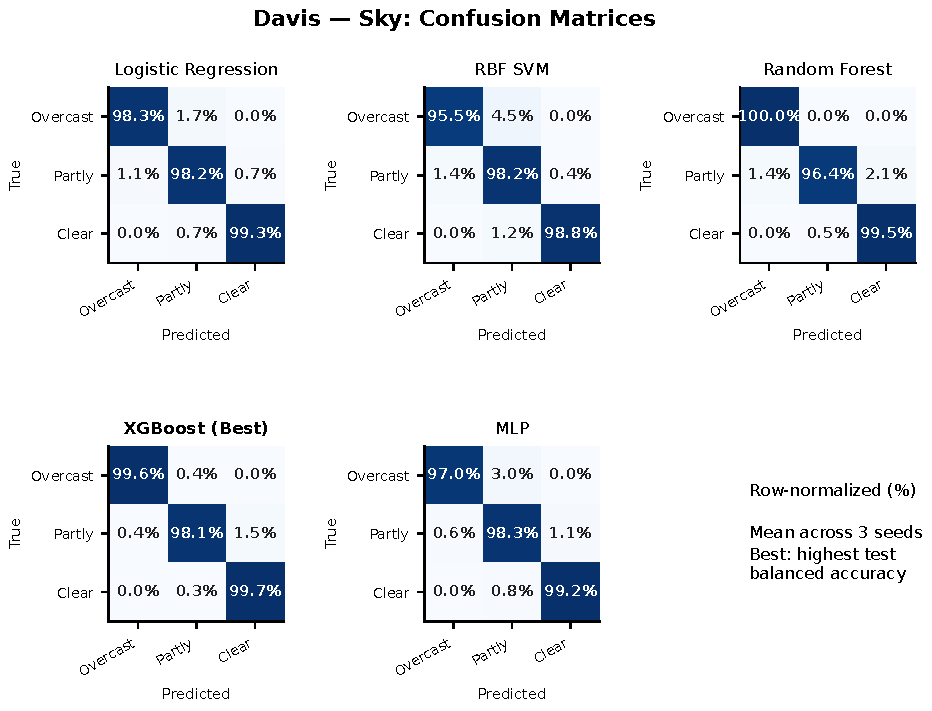
\includegraphics[width=0.78\linewidth]{Figures/P1/P1_Davis_Sky_Confusion.pdf}
  \caption{Davis sky conditions}
\end{subfigure}
\par\medskip
\begin{subfigure}{0.95\textwidth}
  \centering
  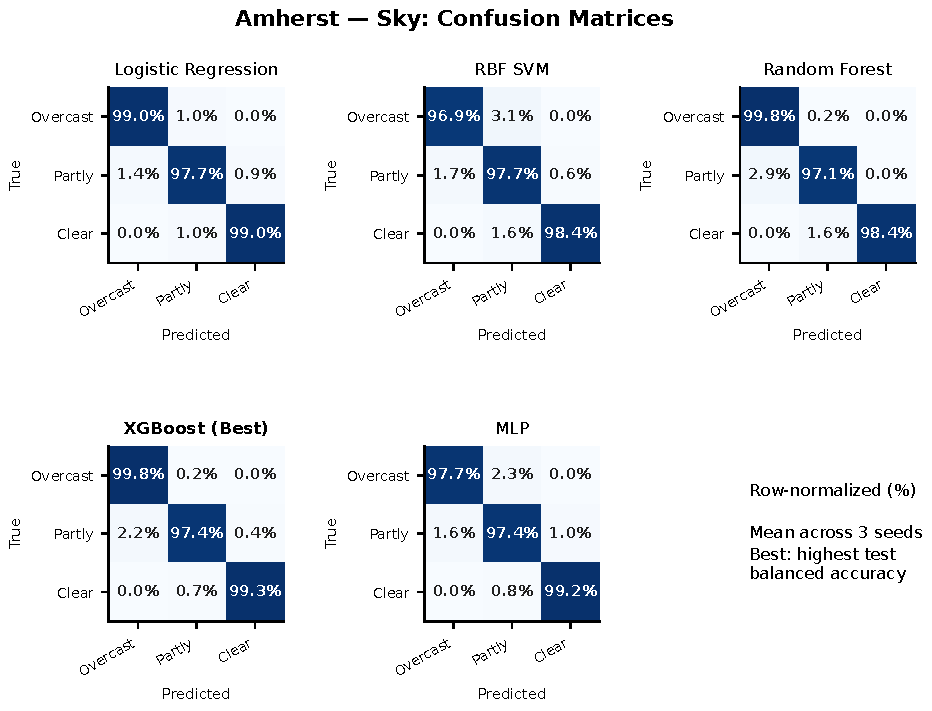
\includegraphics[width=0.78\linewidth]{Figures/P1/P1_Amherst_Sky_Confusion.pdf}
  \caption{Amherst sky conditions}
\end{subfigure}
\caption{P1 sky-condition confusion matrices for Davis and Amherst.
Correct classifications appear on the diagonal; off-diagonal entries show
confusion among Clear, Partly Cloudy, and Overcast conditions.}
\label{fig:p1skyconf}
\end{figure}

\begin{figure}[!htbp]
\centering
\begin{subfigure}{0.95\textwidth}
  \centering
  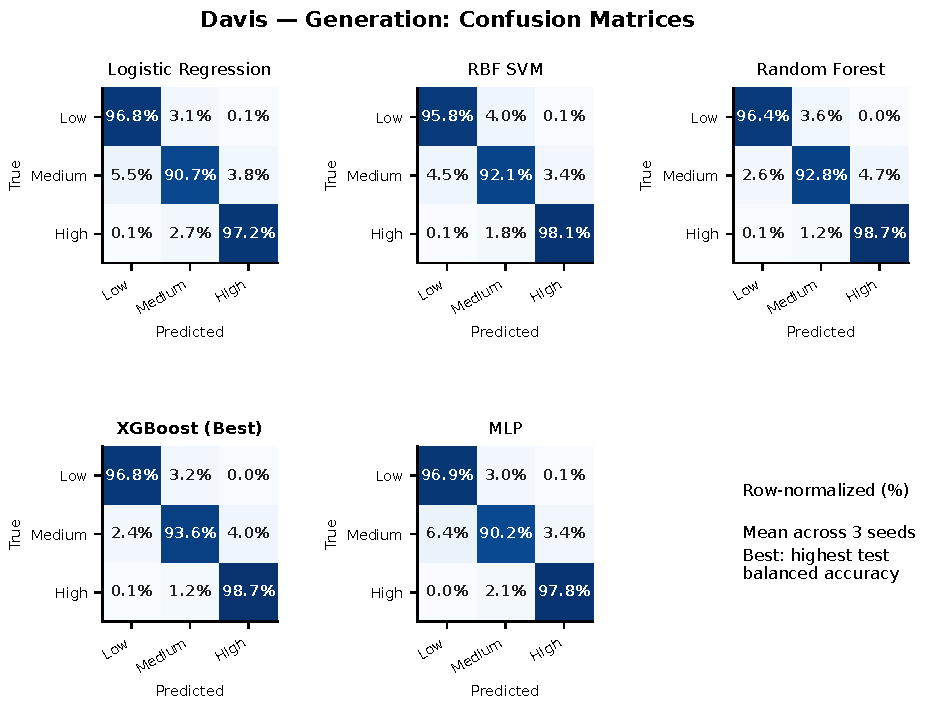
\includegraphics[width=0.78\linewidth]{Figures/P1/P1_Davis_Generation_Confusion.pdf}
  \caption{Davis generation regimes}
\end{subfigure}
\par\medskip
\begin{subfigure}{0.95\textwidth}
  \centering
  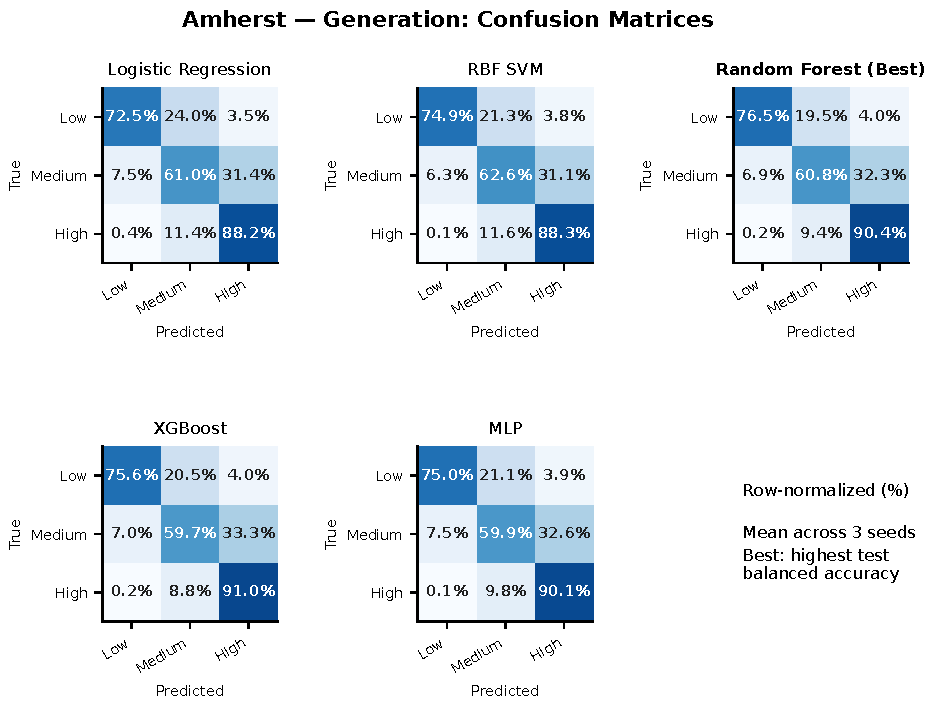
\includegraphics[width=0.78\linewidth]{Figures/P1/P1_Amherst_Generation_Confusion.pdf}
  \caption{Amherst generation regimes}
\end{subfigure}
\caption{P1 generation-regime confusion matrices for Davis and
Amherst. Off-diagonal entries identify errors between Low, Medium, and
High PV-output classes.}
\label{fig:p1genconf}
\end{figure}

\paragraph{Per-class performance.}
Table~\ref{tab:p1recall} extracts the per-class recall of the best test classifier for each
city and task from Figures~\ref{fig:p1skyconf} and~\ref{fig:p1genconf}.
\begin{table}[!htbp]\centering\footnotesize
\caption{P1 per-class recall (\%, row-normalized held-out confusion matrices,
mean over three seeds). The hardest class in each row is shaded in gold. These are
recalls, not per-class precision or F1.}\label{tab:p1recall}
\setlength{\tabcolsep}{5pt}
\begin{tabular}{@{}lllrrr@{}}\toprule
\textbf{City} & \textbf{Task} & \textbf{Best test model} & \textbf{Class 1} & \textbf{Class 2} & \textbf{Class 3}\\\midrule
Davis & Sky & XGBoost & 99.6 & \cellcolor{gold!17}\textbf{98.1} & 99.7\\
Amherst & Sky & XGBoost & 99.8 & \cellcolor{gold!17}\textbf{97.4} & 99.3\\
Davis & Generation & XGBoost & 96.8 & \cellcolor{gold!17}\textbf{93.6} & 98.7\\
Amherst & Generation & Random forest & 76.5 & \cellcolor{gold!17}\textbf{60.8} & 90.4\\
\bottomrule\end{tabular}
\par\smallskip{\scriptsize Sky classes: 1 = Overcast, 2 = Partly Cloudy,
3 = Clear. Generation classes: 1 = Low, 2 = Medium, 3 = High.}
\end{table}

\subsection{Analysis: which classes are hardest and why}
\paragraph{The middle class is always hardest.} In every city and task, the hardest class is the
one in the middle of the ordinal scale: Partly Cloudy for sky and Medium for generation. These
classes have \emph{two} decision boundaries, so a sample can be misclassified in either direction,
while Overcast/Low and Clear/High have only one neighbour. Samples close to a threshold
($k\approx0.4$, $k\approx0.85$, or a power tercile) are inherently ambiguous, and the band
$0.4\le k<0.85$ also mixes physically different situations (thin overcast, broken cumulus,
cloud-edge brightening).

\paragraph{Amherst generation is a weather-to-power problem, not a weather-sensing problem.}
Amherst sky classification is nearly perfect ($98.82\%$), so its weather inputs are informative.
Yet the Amherst Medium regime is recognized only $60.8\%$ of the time, and its errors are
asymmetric: about $32\%$ of true-Medium samples are predicted High but only $\approx7\%$ are
predicted Low (Figure~\ref{fig:p1genconf}b). The same weather therefore maps to a wider range of
output in Amherst than in Davis. Factors that are not in the feature set---for example snow or
soiling on the panels, module temperature, inverter clipping or array downtime---are plausible
causes. P2 corroborates this: the same-city regression error is $15.7\%$ nRMSE in Amherst versus
$4.7\%$ in Davis.

\paragraph{Model families.} Tree ensembles (XGBoost or random forest) give the best test score in
all four city/task combinations; the MLP is never best on test data, although it is
validation-selected in Amherst. Linear logistic regression is within
$0.6$ points of the best sky model, which indicates that the sky task is close to linearly
separable once DHI/DNI and clear-sky values are available.

\paragraph{Caution on the sky score.} High sky accuracy describes \emph{nowcasting} from
simultaneous measurements; it is not a forecast of future sky condition. Removing Output Power
(\texttt{Sky\_NoPower}) leaves the scores unchanged (Section~\ref{sec:p3}), so power is not the
shortcut, but physical irradiance proxies remain (Section~\ref{sec:discussion}).
\FloatBarrier

% =================================================================
\section{P2: Supervised PV Power Regression}\label{sec:p2}

\subsection{Objective and tasks}
P2 predicts continuous Output Power (kW) under four protocols: (i) same-city prediction with a
chronological 80/20 split (Davis, Amherst); (ii) zero-shot cross-city generalization from Davis
(six years) to Huron, Santa Barbara and La Jolla; (iii) sequential forecasting, in which the
previous $K=12$ steps predict the next step; and (iv) a three- versus six-year history ablation.
These protocols use different information and are reported separately, not as one leaderboard.

\subsection{Preprocessing}
Output Power is the label and is excluded from contemporaneous inputs. For same-city prediction,
scaling and encoding are fitted on the earlier training partition and applied to that city's
held-out observations (Figure~\ref{fig:preprocess}). \textbf{In the zero-shot protocol, the
preprocessing fitted on Davis training inputs is reused for the target-city inputs}, and the
Davis-trained predictor is evaluated without any target-city fitting, label calibration or use of
target labels. The target output is therefore \emph{not} rescaled to the target city's power
level. \textbf{Protocol distinction:} the assignment recommends per-city normalization for P2
cross-city evaluation; the results here instead measure source-scaled, raw-kW zero-shot
prediction, i.e.\ the unadapted deployment case, and are not results of the per-city-normalized
protocol (see Section~\ref{sec:discussion}). For the sequential variant, a 12-step history
window predicts the next output without access to future values. As measurements are taken
only in the mid-day window, \emph{one-step ahead} means the next recorded observation, which
may follow an overnight gap rather than a 30-minute interval.

\subsection{Methods and models}
Ridge regression, RBF support-vector regression (SVR), random forest, XGBoost and a PyTorch MLP
are evaluated in all non-sequential protocols; the sequential protocol replaces the MLP with a
PyTorch LSTM, which consumes the 12-step window directly. Figure~\ref{fig:p2flow} shows the four
protocols as alternative branches, not successive training steps. Tables~\ref{tab:p2methods}
and~\ref{tab:p2impl} list model families and libraries.
\begin{table}[!htbp]\centering\footnotesize
\setlength{\tabcolsep}{5pt}
\caption{P2 model and method inventory, separating classical machine learning and deep learning.}\label{tab:p2methods}
\begin{tabular}{@{}p{0.19\linewidth}p{0.37\linewidth}p{0.34\linewidth}@{}}\toprule
\textbf{Family / stage} & \textbf{Models or strategies} & \textbf{Purpose}\\\midrule
\rowcolor{gold!10}
Classical ML & Ridge regression, RBF SVR & Regularized linear and nonlinear regression\\
\rowcolor{gold!10}
Classical ML & Random forest, XGBoost & Tree ensembles for tabular observations\\
\rowcolor{teal!9}
Deep learning & PyTorch MLP & Feed-forward regression\\
\rowcolor{teal!9}
Deep learning & PyTorch LSTM & Sequence forecasting only\\
\bottomrule\end{tabular}
\end{table}


\begin{table}[!htbp]\centering\footnotesize
\caption{P2 regression libraries and protocol settings. Estimator-specific regularization, tree counts, and neural optimizer settings must be verified from the executed P2 notebook before submission.}\label{tab:p2impl}
\begin{tabularx}{\linewidth}{@{}p{0.24\linewidth}p{0.19\linewidth}X@{}}\toprule
\textbf{Model} & \textbf{Python library} & \textbf{Verified setup}\\\midrule
Ridge; SVR (RBF) & \texttt{scikit-learn} & Regularized linear / RBF-kernel regression.\\
Random forest & \texttt{scikit-learn} & Ensemble regression; three seeds.\\
XGBoost & \texttt{xgboost} & Boosted-tree regression; three seeds.\\
MLP & \texttt{PyTorch} & Feed-forward neural power regressor.\\
LSTM & \texttt{PyTorch} & Sequence model; $12$ historical steps to predict the next output.\\
\bottomrule\end{tabularx}
\end{table}


\begin{figure}[!htbp]\centering
\tikzfit{p2_regression}
\caption{P2 regression protocols and supervised model evaluation. The sequential branch uses historical windows rather than future information.}\label{fig:p2flow}
\end{figure}

\subsection{Results}
\paragraph{Same-city and sequential regression.}
Tables~\ref{tab:p2same} and~\ref{tab:p2seqmodels} report every model. In the same-city protocol,
XGBoost and the MLP tie for Davis at $11.85$\,kW RMSE ($4.72\%$ nRMSE; XGBoost has the smaller
seed variance), and the MLP is best in Amherst at $19.96$\,kW ($15.69\%$). In the sequential
protocol, random forest is best in both cities ($13.30$ and $15.96$\,kW), ahead of the LSTM
($14.64$ and $16.55$\,kW).

\begin{table}[!htbp]\centering\scriptsize
\setlength{\tabcolsep}{3pt}
\caption{P2 same-city regression: all evaluated models (mean $\pm$ SD, kW; three seeds).}\label{tab:p2same}
\begin{tabular}{@{}lrrrr@{}}\toprule
\textbf{Regressor} & \textbf{Davis RMSE} & \textbf{Davis MAE} & \textbf{Amherst RMSE} & \textbf{Amherst MAE}\\\midrule
Ridge & 13.82\,$\pm$\,0.00 & 8.49\,$\pm$\,0.00 & 20.72\,$\pm$\,0.00 & 14.61\,$\pm$\,0.00\\
RBF SVR & 14.14\,$\pm$\,0.00 & 10.03\,$\pm$\,0.00 & 25.79\,$\pm$\,0.00 & 19.52\,$\pm$\,0.00\\
Random forest & 11.95\,$\pm$\,0.01 & 5.75\,$\pm$\,0.01 & 20.17\,$\pm$\,0.04 & 13.58\,$\pm$\,0.02\\
XGBoost & 11.85\,$\pm$\,0.08 & 6.33\,$\pm$\,0.03 & 20.12\,$\pm$\,0.21 & 13.78\,$\pm$\,0.18\\
MLP (PyTorch) & \bestscore{11.85\,$\pm$\,0.27} & 6.52\,$\pm$\,0.44 & \bestscore{19.96\,$\pm$\,0.05} & 14.09\,$\pm$\,0.14\\
\bottomrule\end{tabular}
\end{table}

\begin{table}[!htbp]\centering\scriptsize
\setlength{\tabcolsep}{3pt}
\caption{P2 sequential regression: all evaluated models (mean $\pm$ SD, kW; three seeds).}\label{tab:p2seqmodels}
\begin{tabular}{@{}lrrrr@{}}\toprule
\textbf{Regressor} & \textbf{Davis RMSE} & \textbf{Davis MAE} & \textbf{Amherst RMSE} & \textbf{Amherst MAE}\\\midrule
Ridge & 13.58\,$\pm$\,0.00 & 7.77\,$\pm$\,0.00 & 17.12\,$\pm$\,0.00 & 11.69\,$\pm$\,0.00\\
RBF SVR & 18.48\,$\pm$\,0.00 & 13.24\,$\pm$\,0.00 & 20.41\,$\pm$\,0.00 & 15.15\,$\pm$\,0.00\\
Random forest & \bestscore{13.30\,$\pm$\,0.04} & 6.40\,$\pm$\,0.02 & \bestscore{15.96\,$\pm$\,0.05} & 10.63\,$\pm$\,0.03\\
XGBoost & 13.49\,$\pm$\,0.05 & 6.73\,$\pm$\,0.05 & 16.06\,$\pm$\,0.09 & 10.75\,$\pm$\,0.01\\
LSTM (PyTorch) & 14.64\,$\pm$\,0.35 & 8.07\,$\pm$\,0.27 & 16.55\,$\pm$\,0.34 & 11.42\,$\pm$\,0.39\\
\bottomrule\end{tabular}
\end{table}

\begin{table}[!htbp]\centering\scriptsize
\setlength{\tabcolsep}{3pt}
\caption{P2 all-model zero-shot comparisons: train on Davis and test without target fine-tuning (RMSE in kW, mean $\pm$ SD). Davis is the in-domain reference.}\label{tab:p2cross}
\begin{tabular}{@{}lrrrr@{}}\toprule
\textbf{Regressor} & \textbf{Davis (ID)} & \textbf{Huron} & \textbf{La Jolla} & \textbf{Santa Barbara}\\\midrule
Ridge & 16.95\,$\pm$\,0.00 & 124.95\,$\pm$\,0.00 & 130.18\,$\pm$\,0.00 & 126.01\,$\pm$\,0.00\\
RBF SVR & 16.32\,$\pm$\,0.00 & \bestscore{114.61\,$\pm$\,0.00} & \bestscore{77.27\,$\pm$\,0.00} & \bestscore{102.96\,$\pm$\,0.00}\\
Random forest & 15.21\,$\pm$\,0.02 & 124.49\,$\pm$\,0.04 & 124.75\,$\pm$\,0.08 & 125.03\,$\pm$\,0.02\\
XGBoost & \bestscore{14.88\,$\pm$\,0.07} & 125.72\,$\pm$\,0.08 & 121.48\,$\pm$\,2.92 & 121.11\,$\pm$\,1.68\\
MLP (PyTorch) & 15.19\,$\pm$\,0.06 & 123.57\,$\pm$\,1.38 & 123.47\,$\pm$\,6.07 & 120.76\,$\pm$\,2.09\\
\bottomrule\end{tabular}
\end{table}

\begin{table}[!htbp]\centering\tiny
\setlength{\tabcolsep}{2pt}
\caption{P2 three- versus six-year comparison for every regressor (mean $\pm$ SD nRMSE, \%). Lower is better; bold identifies the best within each city/history configuration.}\label{tab:p2history}
\begin{tabular}{@{}lrrrrrrrr@{}}\toprule
\textbf{Regressor} & \multicolumn{2}{c}{\textbf{Davis}} & \multicolumn{2}{c}{\textbf{Huron}} & \multicolumn{2}{c}{\textbf{La Jolla}} & \multicolumn{2}{c}{\textbf{Santa Barbara}}\\\cmidrule(lr){2-3}\cmidrule(lr){4-5}\cmidrule(lr){6-7}\cmidrule(lr){8-9}
 & 3yr & 6yr & 3yr & 6yr & 3yr & 6yr & 3yr & 6yr\\\midrule
Ridge & 5.50\,$\pm$\,0.00 & 5.63\,$\pm$\,0.00 & 5.02\,$\pm$\,0.00 & 5.33\,$\pm$\,0.00 & 9.32\,$\pm$\,0.00 & 9.09\,$\pm$\,0.00 & \bestscore{12.09\,$\pm$\,0.00} & 12.85\,$\pm$\,0.00\\
RBF SVR & 5.63\,$\pm$\,0.00 & 4.86\,$\pm$\,0.00 & 5.41\,$\pm$\,0.00 & 4.95\,$\pm$\,0.00 & 10.00\,$\pm$\,0.00 & 9.66\,$\pm$\,0.00 & 14.90\,$\pm$\,0.00 & 12.73\,$\pm$\,0.00\\
Random forest & 4.76\,$\pm$\,0.01 & 4.70\,$\pm$\,0.02 & 4.79\,$\pm$\,0.00 & 4.65\,$\pm$\,0.02 & 8.16\,$\pm$\,0.02 & 8.03\,$\pm$\,0.02 & 12.93\,$\pm$\,0.07 & 13.83\,$\pm$\,0.05\\
XGBoost & 4.72\,$\pm$\,0.03 & 4.70\,$\pm$\,0.04 & 4.58\,$\pm$\,0.05 & \bestscore{4.47\,$\pm$\,0.01} & \bestscore{8.16\,$\pm$\,0.04} & \bestscore{7.87\,$\pm$\,0.08} & 12.24\,$\pm$\,0.02 & 12.74\,$\pm$\,0.10\\
MLP (PyTorch) & \bestscore{4.72\,$\pm$\,0.11} & \bestscore{4.58\,$\pm$\,0.08} & \bestscore{4.49\,$\pm$\,0.06} & 4.57\,$\pm$\,0.08 & 8.69\,$\pm$\,0.49 & 7.99\,$\pm$\,0.08 & 13.03\,$\pm$\,0.33 & \bestscore{12.27\,$\pm$\,0.40}\\
\bottomrule\end{tabular}
\end{table}



Figure~\ref{fig:p2traces} overlays predictions and measurements on the held-out period. The
models follow the daily shape closely; the largest residuals occur during rapid ramps, when
cloud passages change output within one 30-minute interval.

\begin{figure}[!htbp]\centering
\begin{subfigure}[b]{0.48\textwidth}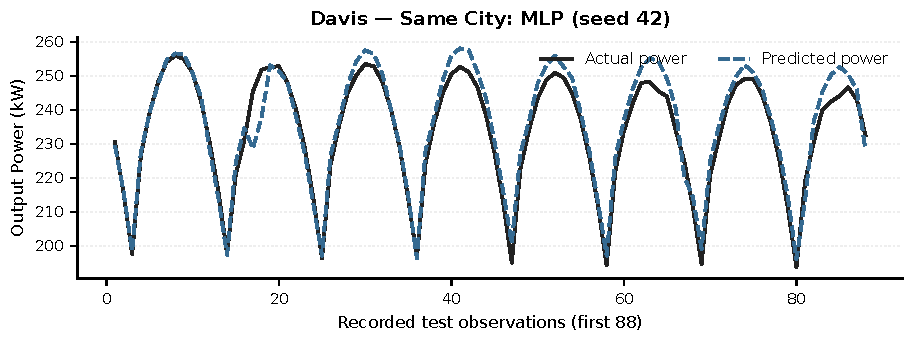
\includegraphics[width=\linewidth]{Figures/P2/P2_Same_City_Davis_Prediction_Trace.pdf}\caption{Davis}\end{subfigure}\hfill
\begin{subfigure}[b]{0.48\textwidth}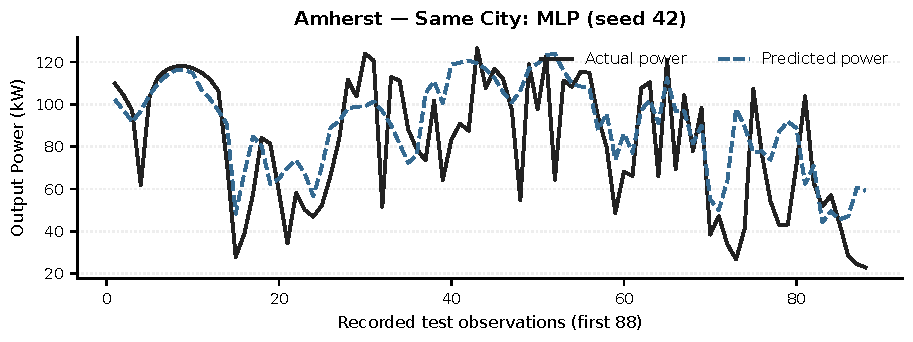
\includegraphics[width=\linewidth]{Figures/P2/P2_Same_City_Amherst_Prediction_Trace.pdf}\caption{Amherst}\end{subfigure}
\caption{Prediction-versus-truth traces for the same-city experiments (MLP, seed 42).}\label{fig:p2traces}
\end{figure}

\paragraph{Cross-city zero-shot evaluation and site power scales.}
Table~\ref{tab:citypower} makes the physical-scale shift explicit. Davis averages $164.02$\,kW
over its six-year sheet, versus $50.11$, $49.08$ and $47.26$\,kW for Huron, Santa Barbara and
La Jolla, i.e. $3.3$--$3.5\times$ more. These are measured statistics from the workbook, not model
outputs. Amherst is included for the related P5 experiments.
\begin{table}[!htbp]
\centering\small
\caption{Measured PV output scale across cities. The full-sheet mean uses all non-missing Output Power observations; held-out means use each sheet's chronological last 20\%. Davis is the source for P2 zero-shot tests; Amherst is the P5 transfer target.}
\label{tab:citypower}
\setlength{\tabcolsep}{5pt}
\begin{tabular}{@{}llrrr@{}}\toprule
\textbf{City} & \textbf{Period} & \textbf{Full-sheet mean (kW)} & \textbf{Held-out mean (kW)} & \textbf{Davis / city}\\\midrule
\rowcolor{gold!13} Davis (source) & 2011--2016 & \textbf{164.02} & 150.51 & 1.00\\
Huron & 2011--2016 & 50.11 & 47.92 & 3.27\\
Santa Barbara & 2011--2016 & 49.08 & 48.36 & 3.34\\
La Jolla & 2011--2016 & 47.26 & 46.14 & 3.47\\
Amherst (P5 target) & 2018--2020 & 60.93 & 63.71 & 2.69\\
\bottomrule\end{tabular}
\end{table}

Table~\ref{tab:p2cross} reports all five models for each target. Every zero-shot error is roughly
an order of magnitude larger than the Davis in-domain reference. Figure~\ref{fig:p2crossplot}
shows nRMSE by model and site, and Figure~\ref{fig:p2powerbias} compares predicted and actual mean
power: even the best zero-shot model predicts Davis-sized output (mean $122$--$155$\,kW) for sites
that produce about $46$--$48$\,kW. The strong overprediction indicates a systematic output-scale bias in this
raw-kW protocol, alongside possible weather and feature-distribution differences.

\fign{Figures/P2/P2_Cross_City_All_Models.pdf}{Cross-city zero-shot nRMSE across regression methods and target sites.}{fig:p2crossplot}
\fign{Figures/P2/P2_Cross_City_Power_Bias.pdf}{Source-to-target power bias in the zero-shot study: mean predicted versus actual output for the best model per site; compare with Table~\ref{tab:citypower}.}{fig:p2powerbias}

\paragraph{Three-year versus six-year history.}
Table~\ref{tab:p2history} reports all five models for both histories in four cities, and
Figure~\ref{fig:p2historyplot} shows the best model per configuration. Six years improve the best
nRMSE slightly in Davis ($4.72\to4.58\%$), Huron ($4.49\to4.47\%$) and La Jolla ($8.16\to7.87\%$)
but not in Santa Barbara ($12.09\to12.27\%$). The gains are an order of magnitude smaller than the
cross-city errors.

\fign{Figures/P2/P2_Three_vs_Six_Years_Best_Models.pdf}{Best-model nRMSE for the matched three-year versus six-year history study.}{fig:p2historyplot}

\paragraph{Supplementary MAE results for all P2 setups.}
The same-city and sequential MAE values appear alongside RMSE in
Tables~\ref{tab:p2same} and~\ref{tab:p2seqmodels}. The missing zero-shot
and history-ablation MAE values are provided in Tables~\ref{tab:p2crossmae}
and~\ref{tab:p2historymae}, respectively; every model and target is shown,
with the same three-seed protocol.

\begin{table}[H]\centering\scriptsize
\setlength{\tabcolsep}{3.4pt}\renewcommand{\arraystretch}{1.16}
\caption{P2 cross-city zero-shot MAE in kW, all models (mean $\pm$ SD over three seeds). The Davis column is the source-city in-domain reference; the remaining columns use the unchanged Davis-trained predictor.}
\label{tab:p2crossmae}
\begin{tabular}{@{}lrrrr@{}}\toprule
\textbf{Model} & \textbf{Davis (ID)} & \textbf{Huron} & \textbf{Santa Barbara} & \textbf{La Jolla}\\\midrule
Ridge & 9.79\,$\pm$\,0.00 & 115.24\,$\pm$\,0.00 & 117.31\,$\pm$\,0.00 & 122.02\,$\pm$\,0.00 \\
RBF SVR & 10.04\,$\pm$\,0.00 & 107.38\,$\pm$\,0.00 & 98.68\,$\pm$\,0.00 & 75.88\,$\pm$\,0.00 \\
Random forest & 7.90\,$\pm$\,0.01 & 115.35\,$\pm$\,0.08 & 115.85\,$\pm$\,0.04 & 115.98\,$\pm$\,0.09 \\
XGBoost & 8.12\,$\pm$\,0.04 & 116.62\,$\pm$\,0.13 & 112.11\,$\pm$\,1.36 & 113.30\,$\pm$\,2.54 \\
MLP (PyTorch) & 8.68\,$\pm$\,0.14 & 114.23\,$\pm$\,0.50 & 113.34\,$\pm$\,2.46 & 118.19\,$\pm$\,6.75 \\
\bottomrule\end{tabular}
\end{table}


\begin{longtable}{@{}llrr@{}}
\caption{P2 three- versus six-year ablation: held-out MAE in kW for every model (mean $\pm$ SD, three seeds). The corresponding RMSE and nRMSE comparisons appear in Table~\ref{tab:p2history}.}\label{tab:p2historymae}\\
\toprule\textbf{City} & \textbf{Regressor} & \textbf{3-year MAE} & \textbf{6-year MAE}\\\midrule
\endfirsthead
\multicolumn{4}{l}{\footnotesize Table \thetable\ (continued)}\\
\toprule\textbf{City} & \textbf{Regressor} & \textbf{3-year MAE} & \textbf{6-year MAE}\\\midrule
\endhead
Davis & Ridge & 8.49\,$\pm$\,0.00 & 8.25\,$\pm$\,0.00 \\
Davis & RBF SVR & 10.03\,$\pm$\,0.00 & 6.86\,$\pm$\,0.00 \\
Davis & Random forest & 5.75\,$\pm$\,0.01 & 5.59\,$\pm$\,0.03 \\
Davis & XGBoost & 6.33\,$\pm$\,0.03 & 6.35\,$\pm$\,0.13 \\
Davis & MLP (PyTorch) & 6.52\,$\pm$\,0.44 & 6.16\,$\pm$\,0.13 \\
\addlinespace[2pt]
Huron & Ridge & 2.01\,$\pm$\,0.00 & 2.32\,$\pm$\,0.00 \\
Huron & RBF SVR & 2.52\,$\pm$\,0.00 & 2.13\,$\pm$\,0.00 \\
Huron & Random forest & 1.87\,$\pm$\,0.00 & 1.84\,$\pm$\,0.00 \\
Huron & XGBoost & 1.85\,$\pm$\,0.02 & 1.78\,$\pm$\,0.00 \\
Huron & MLP (PyTorch) & 1.88\,$\pm$\,0.06 & 1.89\,$\pm$\,0.04 \\
\addlinespace[2pt]
Santa Barbara & Ridge & 6.23\,$\pm$\,0.00 & 7.01\,$\pm$\,0.00 \\
Santa Barbara & RBF SVR & 7.02\,$\pm$\,0.00 & 5.90\,$\pm$\,0.00 \\
Santa Barbara & Random forest & 6.01\,$\pm$\,0.01 & 6.61\,$\pm$\,0.02 \\
Santa Barbara & XGBoost & 5.96\,$\pm$\,0.04 & 6.24\,$\pm$\,0.04 \\
Santa Barbara & MLP (PyTorch) & 6.53\,$\pm$\,0.35 & 5.97\,$\pm$\,0.24 \\
\addlinespace[2pt]
La Jolla & Ridge & 4.54\,$\pm$\,0.00 & 4.37\,$\pm$\,0.00 \\
La Jolla & RBF SVR & 5.03\,$\pm$\,0.00 & 4.74\,$\pm$\,0.00 \\
La Jolla & Random forest & 3.75\,$\pm$\,0.01 & 3.80\,$\pm$\,0.01 \\
La Jolla & XGBoost & 3.88\,$\pm$\,0.01 & 3.74\,$\pm$\,0.05 \\
La Jolla & MLP (PyTorch) & 4.33\,$\pm$\,0.28 & 3.75\,$\pm$\,0.06 \\
\addlinespace[2pt]
\bottomrule
\end{longtable}


\paragraph{Normalized error.}
Tables~\ref{tab:p2nrmse},~\ref{tab:p2seqnrmse} and~\ref{tab:p2nrmsecross} give the nRMSE that
corresponds to the kW tables above (mean $\pm$ SD over three seeds).

\begin{table}[!htbp]\centering\scriptsize
\setlength{\tabcolsep}{4pt}
\begin{minipage}[t]{0.46\textwidth}\centering
\caption{Same-city nRMSE (\%).}\label{tab:p2nrmse}
\begin{tabular}{@{}lrr@{}}\toprule
\textbf{Model} & \textbf{Davis} & \textbf{Amherst}\\\midrule
Ridge & 5.50\,$\pm$\,0.00 & 16.29\,$\pm$\,0.00\\
RBF SVR & 5.63\,$\pm$\,0.00 & 20.28\,$\pm$\,0.00\\
Random forest & 4.76\,$\pm$\,0.01 & 15.86\,$\pm$\,0.03\\
XGBoost & \textbf{4.72\,$\pm$\,0.03} & 15.82\,$\pm$\,0.17\\
MLP (PyTorch) & \textbf{4.72\,$\pm$\,0.11} & \textbf{15.69\,$\pm$\,0.04}\\
\bottomrule\end{tabular}
\end{minipage}\hfill
\begin{minipage}[t]{0.50\textwidth}\centering
\caption{Sequential ($K=12$) nRMSE (\%).}\label{tab:p2seqnrmse}
\begin{tabular}{@{}lrr@{}}\toprule
\textbf{Model} & \textbf{Davis} & \textbf{Amherst}\\\midrule
Ridge & 5.40\,$\pm$\,0.00 & 13.46\,$\pm$\,0.00\\
RBF SVR & 7.36\,$\pm$\,0.00 & 16.04\,$\pm$\,0.00\\
Random forest & \textbf{5.29\,$\pm$\,0.01} & \textbf{12.54\,$\pm$\,0.04}\\
XGBoost & 5.37\,$\pm$\,0.02 & 12.62\,$\pm$\,0.07\\
LSTM (PyTorch) & 5.83\,$\pm$\,0.14 & 13.01\,$\pm$\,0.27\\
\bottomrule\end{tabular}
\end{minipage}
\end{table}
\begin{table}[!htbp]\centering\scriptsize
\setlength{\tabcolsep}{4pt}
\caption{Cross-city zero-shot nRMSE (\%); Davis is the in-domain reference.}\label{tab:p2nrmsecross}
\begin{tabular}{@{}lrrrr@{}}\toprule
\textbf{Model} & \textbf{Davis (ID)} & \textbf{Huron} & \textbf{La Jolla} & \textbf{Santa Barbara}\\\midrule
Ridge & 6.71\,$\pm$\,0.00 & 168.05\,$\pm$\,0.00 & 189.90\,$\pm$\,0.00 & 170.66\,$\pm$\,0.00\\
RBF SVR & 6.46\,$\pm$\,0.00 & \textbf{154.14\,$\pm$\,0.00} & \textbf{112.72\,$\pm$\,0.00} & \textbf{139.44\,$\pm$\,0.00}\\
Random forest & 6.02\,$\pm$\,0.01 & 167.44\,$\pm$\,0.06 & 181.98\,$\pm$\,0.11 & 169.33\,$\pm$\,0.03\\
XGBoost & \textbf{5.89\,$\pm$\,0.03} & 169.09\,$\pm$\,0.10 & 177.21\,$\pm$\,4.26 & 164.02\,$\pm$\,2.27\\
MLP (PyTorch) & 6.01\,$\pm$\,0.02 & 166.19\,$\pm$\,1.86 & 180.11\,$\pm$\,8.86 & 163.54\,$\pm$\,2.84\\
\bottomrule\end{tabular}
\end{table}

\subsection{Analysis and observations}
\paragraph{Why tree ensembles and the MLP win in-city.} Output Power is a smooth but strongly
non-linear function of a few irradiance variables (DNI, DHI, zenith angle) with interactions
(e.g. temperature only matters when irradiance is high). Random forests and XGBoost represent such
piecewise interactions without feature engineering, which is why they cut Ridge's error by about
$14\%$ in Davis. The MLP matches them but with larger seed variance.

\paragraph{Why RBF SVR is the ``least bad'' zero-shot model.} SVR is mid-table in-city but best on
all three unseen sites. A plausible explanation is that an RBF model's prediction relaxes towards
its bias term for inputs far from the training support, which limits how far it extrapolates the
Davis scale. The SVR advantage is largest at La Jolla ($112.7\%$ versus $177$--$190\%$ nRMSE for the
other models), which is also where its mean prediction is lowest ($122$\,kW,
Figure~\ref{fig:p2powerbias}). This is a weaker over-prediction, not a solution: the error remains
above $100\%$ nRMSE.

\paragraph{Sequence information matters most where weather explains least.} In Amherst, the
12-step sequential model ($15.96$\,kW) has lower error than the contemporaneous same-city model
($19.96$\,kW), whereas in Davis the order is reversed ($13.30$ vs $11.85$\,kW). The two protocols
do not use identical inputs, so this is not a strict comparison, but it is consistent with P1:
where weather variables explain power poorly (Amherst), recent output carries site-specific
information---availability, soiling, snow---that the weather columns lack.

\paragraph{The LSTM does not beat random forest.} With only a 12-step window and tabular inputs,
a tree ensemble over flattened lags is as expressive as the LSTM and easier to fit; the LSTM also
shows the largest seed variance.

\paragraph{More history helps a little.} Doubling the history from three to six years helps
three of four cities by at most $0.3$ nRMSE points, suggesting that three years already cover the
seasonal range of conditions; Santa Barbara, the coastal site with the highest error, does not
benefit.
\FloatBarrier

% =================================================================
\section{P3: Dimensionality Reduction for Classification and Regression}\label{sec:p3}

\subsection{Objective and tasks}
P3 asks whether a lower-dimensional representation keeps enough information for the P1
classifiers and the P2 regressor. Preprocessed predictors are compressed to $d\in\{2,5,10\}$
dimensions without labels, and \emph{reduce-then-predict} is compared with prediction from the
full input vector. Both intrinsic quality (variance retained, reconstruction error) and downstream
utility (BA, accuracy, RMSE, MAE) are evaluated.

\subsection{Preprocessing}
The same chronological partitions and task-specific exclusions as P1/P2 are used. Standardization
and Cloud Type encoding are fitted on training data before fitting a reducer. PCA, kernel PCA
and the autoencoder are fitted on training \emph{predictors} only---never on labels and never on
test data---and are then used to transform both partitions. t-SNE and UMAP maps use training
observations only and do not contribute to any score.

\subsection{Methods and models}
Three reducers are compared: (i) linear PCA; (ii) approximate RBF kernel PCA via a Nystr\"om
feature map (192 landmarks); and (iii) a PyTorch autoencoder with encoder $p\to64\to32\to d$ and a
symmetric decoder. The same five downstream classifiers/regressors as in P1/P2 are trained on each
reduced representation. Figure~\ref{fig:p3flow} separates unsupervised compression from
supervised prediction; Tables~\ref{tab:p3methods} and~\ref{tab:p3impl} give methods and saved
hyperparameters.
\begin{table}[!htbp]\centering\footnotesize
\setlength{\tabcolsep}{5pt}
\caption{P3 model and method inventory, separating classical machine learning and deep learning.}\label{tab:p3methods}
\begin{tabular}{@{}p{0.19\linewidth}p{0.37\linewidth}p{0.34\linewidth}@{}}\toprule
\textbf{Family / stage} & \textbf{Models or strategies} & \textbf{Purpose}\\\midrule
\rowcolor{gold!10}
Classical / unsupervised & PCA; approximate RBF kernel PCA & Fit predictors without labels\\
\rowcolor{teal!9}
Deep / unsupervised & PyTorch autoencoder & Learn reconstruction bottlenecks\\
\rowcolor{gold!10}
Classical / downstream & Logistic/Ridge, SVM/SVR, RF, XGBoost & Evaluate learned features\\
\rowcolor{teal!9}
Deep / downstream & PyTorch MLP & Classification and regression\\
\rowcolor{mist}
Visualization only & t-SNE, UMAP & 2D class-colored projections\\
\bottomrule\end{tabular}
\end{table}


\begin{table}[!htbp]\centering\scriptsize
\caption{P3 implementation and major saved hyperparameters. $p$ denotes encoded input dimension and $d$ the compressed dimension. Three seeds were used for the autoencoder and downstream experiments.}\label{tab:p3impl}
\begin{tabularx}{\linewidth}{@{}p{0.23\linewidth}p{0.19\linewidth}X@{}}\toprule
\textbf{Method} & \textbf{Python library} & \textbf{Verified settings}\\\midrule
PCA & \texttt{scikit-learn} & $d\in\{2,5,10\}$; fit to training inputs only.\\
RBF kernel PCA (approx.) & \texttt{scikit-learn} & Nystr\"om feature approximation, 192 landmarks, RBF $\gamma=1/p$; ridge reconstruction decoder $\alpha=1$.\\
Autoencoder & \texttt{PyTorch} & Encoder widths $p\to64\to32\to d$ and symmetric decoder; 35 epochs, batch size 1024, AdamW.\\
UMAP (visualization) & \texttt{umap-learn} & $n_{\mathrm{neighbors}}=25$, $\mathrm{min\_dist}=0.1$, 150 epochs, up to 6000 training samples for fitting.\\
t-SNE (visualization) & \texttt{scikit-learn} & Perplexity 30; 2500 training observations per plotted city/task.\\
Downstream ML models & \texttt{scikit-learn}, \texttt{xgboost}, \texttt{PyTorch} & Logistic max iterations 1500; RBF SVM $C=3$; random forest 160 trees; XGBoost 200 trees and depth 4; MLP hidden widths 64, 32.\\
\bottomrule\end{tabularx}
\end{table}


\begin{figure}[!htbp]\centering
\tikzfit{p3_dimred}
\caption{P3 unsupervised compression followed by supervised downstream testing. Representations are fitted using training features only.}\label{fig:p3flow}
\end{figure}

\subsection{Results}
\paragraph{Intrinsic representation quality.}
Figure~\ref{fig:p3variance} shows cumulative PCA explained variance, and
Figure~\ref{fig:p3reconstruction} shows held-out reconstruction MSE as a function of $d$. The
autoencoder reaches the lowest Davis reconstruction error at small bottlenecks, but, as shown
below, lower reconstruction error does not guarantee better prediction.

\fign{Figures/P3/P3_Final_PCA_Explained_Variance.pdf}{Retained variance as a function of PCA dimensionality for Davis and Amherst tasks.}{fig:p3variance}
\fign{Figures/P3/P3_Final_Reconstruction_Comparison.pdf}{Held-out reconstruction error for PCA, kernel PCA, and autoencoder representations.}{fig:p3reconstruction}

\paragraph{Choosing $d$.}
Table~\ref{tab:p3var} lists the variance retained at each required dimension. The curve has no
sharp elbow, but its slope halves after $d=5$: for Davis sky, components 3--5 add about $9.8$
points each, while components 6--10 add only about $4.2$ points each. Ten components retain
$84$--$86\%$ of input variance and do not reach the conventional $90\%$ threshold. Downstream
results confirm the choice: $d=10$ gives the best reduced score in seven of eight city/task
settings, and $d=5$ is best only for Davis generation. We therefore recommend $d=10$ as the
operating point, with $d=5$ as the knee of the variance curve. Kernel PCA percentages are
measured in kernel space and are not comparable with the PCA column.
\begin{table}[!htbp]\centering\footnotesize
\caption{Retained cumulative variance (\%). Kernel PCA columns measure variance in the approximate kernel representation, not original-feature variance.}\label{tab:p3var}
\begin{tabular}{@{}llrrr@{}}\toprule
\textbf{City} & \textbf{Task} & $d$ & \textbf{PCA (input)} & \textbf{Kernel PCA (kernel)}\\\midrule
Davis & Sky & 2 & 34.29 & 22.36\\
Davis & Sky & 5 & 63.67 & 41.94\\
Davis & Sky & 10 & 84.44 & 57.44\\
Davis & Regression & 2 & 36.92 & 23.30\\
Davis & Regression & 5 & 65.16 & 42.32\\
Davis & Regression & 10 & 85.13 & 57.47\\
Amherst & Sky & 2 & 39.85 & 24.23\\
Amherst & Sky & 5 & 65.88 & 42.46\\
Amherst & Sky & 10 & 85.51 & 57.33\\
Amherst & Regression & 2 & 41.92 & 24.88\\
Amherst & Regression & 5 & 67.21 & 42.91\\
Amherst & Regression & 10 & 86.39 & 57.47\\
\bottomrule\end{tabular}
\end{table}

\paragraph{Downstream prediction.}
Table~\ref{tab:p3} reports the best reduced configuration per city and task against the best
full-feature model trained under the same P3 protocol. The full-feature model wins all eight
comparisons. The penalty is small for generation and regression in Amherst ($-0.50$ BA points and
$+0.28$\,kW) and large for sky classification ($-10.8$ to $-15.0$ BA points).

\begin{table}[!htbp]\centering\small
\caption{Best reduced configuration for each P3 task and city versus the best original-feature model. BA in \%; regression in RMSE (kW). $\Delta$ = reduced $-$ raw (negative BA or positive RMSE means compression hurts).}
\label{tab:p3}
\begin{tabular}{lllrrrr}\toprule
City & Task & Method & $d$ & Reduced & Raw & $\Delta$\\\midrule
Amherst & Generation & Kernel PCA & 10 & 75.56 & 76.06 & $-0.50$\\
Amherst & Regression & Kernel PCA & 10 & 20.25 & 19.97 & $+0.28$\\
Amherst & Sky & PCA & 10 & 88.19 & 98.98 & $-10.79$\\
Amherst & Sky\_NoPower & PCA & 10 & 87.60 & 98.96 & $-11.36$\\
Davis & Generation & PCA & 5 & 90.62 & 94.50 & $-3.88$\\
Davis & Regression & Autoencoder & 10 & 17.85 & 14.93 & $+2.92$\\
Davis & Sky & Autoencoder & 10 & 84.40 & 99.17 & $-14.77$\\
Davis & Sky\_NoPower & Autoencoder & 10 & 84.19 & 99.20 & $-15.01$\\
\bottomrule\end{tabular}
\end{table}

\paragraph{All downstream models at every dimension.}
The complete tables below show every downstream model for $d=2,5,10$, contrasting identical
classifiers/regressors on full, PCA, kernel-PCA and autoencoder inputs. Teal bold marks the best
mean within each representation and dimension.
\begin{table}[!htbp]\centering\scriptsize
\setlength{\tabcolsep}{3pt}
\caption{P3 Davis Sky: all five downstream models at $d=2,5,10$ using original and reduced features (mean $\pm$ SD of balanced accuracy in percent). Bold marks the best model within each representation and dimension; original-feature winner is highlighted.}\label{tab:p3davissky}
\begin{tabular}{@{}r l rrrr@{}}\toprule
\textbf{$d$} & \textbf{Downstream model} & \textbf{Original} & \textbf{PCA} & \textbf{Kernel PCA} & \textbf{Autoencoder}\\\midrule
2 & Logistic regression & 98.44\,$\pm$\,0.00 & 66.92\,$\pm$\,0.00 & 53.15\,$\pm$\,0.00 & 66.20\,$\pm$\,5.94\\
2 & RBF SVM & 97.52\,$\pm$\,0.00 & 67.54\,$\pm$\,0.00 & 61.42\,$\pm$\,0.00 & 77.54\,$\pm$\,3.34\\
2 & Random forest & 98.63\,$\pm$\,0.10 & 64.16\,$\pm$\,0.12 & 54.31\,$\pm$\,0.12 & 76.00\,$\pm$\,1.91\\
2 & XGBoost & \bestscore{99.17\,$\pm$\,0.01} & 66.72\,$\pm$\,0.06 & 59.58\,$\pm$\,0.06 & 73.56\,$\pm$\,2.85\\
2 & MLP (PyTorch) & 97.26\,$\pm$\,0.12 & \bestscore{67.64\,$\pm$\,0.48} & \bestscore{61.85\,$\pm$\,0.14} & \bestscore{77.92\,$\pm$\,3.57}\\
\addlinespace[2pt]\\
5 & Logistic regression & 98.44\,$\pm$\,0.00 & 71.96\,$\pm$\,0.00 & 70.71\,$\pm$\,0.00 & 83.12\,$\pm$\,1.42\\
5 & RBF SVM & 97.52\,$\pm$\,0.00 & \bestscore{78.79\,$\pm$\,0.00} & \bestscore{77.03\,$\pm$\,0.00} & \bestscore{84.13\,$\pm$\,1.25}\\
5 & Random forest & 98.63\,$\pm$\,0.10 & 73.17\,$\pm$\,0.18 & 75.72\,$\pm$\,0.22 & 80.86\,$\pm$\,0.55\\
5 & XGBoost & \bestscore{99.17\,$\pm$\,0.01} & 75.62\,$\pm$\,0.16 & 75.96\,$\pm$\,0.03 & 83.02\,$\pm$\,0.40\\
5 & MLP (PyTorch) & 97.26\,$\pm$\,0.12 & 75.32\,$\pm$\,1.24 & 75.62\,$\pm$\,0.33 & 83.01\,$\pm$\,1.03\\
\addlinespace[2pt]\\
10 & Logistic regression & 98.44\,$\pm$\,0.00 & 80.40\,$\pm$\,0.00 & 80.36\,$\pm$\,0.00 & 83.28\,$\pm$\,0.64\\
10 & RBF SVM & 97.52\,$\pm$\,0.00 & 78.91\,$\pm$\,0.00 & 81.83\,$\pm$\,0.00 & \bestscore{84.40\,$\pm$\,1.65}\\
10 & Random forest & 98.63\,$\pm$\,0.10 & 80.51\,$\pm$\,0.28 & 81.86\,$\pm$\,0.44 & 81.64\,$\pm$\,2.06\\
10 & XGBoost & \bestscore{99.17\,$\pm$\,0.01} & 81.09\,$\pm$\,0.24 & 81.23\,$\pm$\,0.14 & 82.69\,$\pm$\,1.23\\
10 & MLP (PyTorch) & 97.26\,$\pm$\,0.12 & \bestscore{81.66\,$\pm$\,0.77} & \bestscore{81.99\,$\pm$\,0.10} & 84.08\,$\pm$\,2.30\\
\bottomrule\end{tabular}
\end{table}

\begin{table}[!htbp]\centering\scriptsize
\setlength{\tabcolsep}{3pt}
\caption{P3 Davis Sky\_NoPower: all five downstream models at $d=2,5,10$ using original and reduced features (mean $\pm$ SD of balanced accuracy in percent). Bold marks the best model within each representation and dimension; original-feature winner is highlighted.}\label{tab:p3davissky_nopower}
\begin{tabular}{@{}r l rrrr@{}}\toprule
\textbf{$d$} & \textbf{Downstream model} & \textbf{Original} & \textbf{PCA} & \textbf{Kernel PCA} & \textbf{Autoencoder}\\\midrule
2 & Logistic regression & 98.42\,$\pm$\,0.00 & 62.08\,$\pm$\,0.00 & 49.89\,$\pm$\,0.00 & 55.25\,$\pm$\,4.23\\
2 & RBF SVM & 97.24\,$\pm$\,0.00 & 62.19\,$\pm$\,0.00 & 55.38\,$\pm$\,0.00 & 68.91\,$\pm$\,7.08\\
2 & Random forest & 98.67\,$\pm$\,0.07 & 58.78\,$\pm$\,0.39 & 46.77\,$\pm$\,0.15 & 67.94\,$\pm$\,4.15\\
2 & XGBoost & \bestscore{99.20\,$\pm$\,0.04} & \bestscore{63.41\,$\pm$\,0.21} & 55.68\,$\pm$\,0.35 & 65.94\,$\pm$\,3.80\\
2 & MLP (PyTorch) & 98.09\,$\pm$\,0.16 & 63.37\,$\pm$\,0.09 & \bestscore{55.72\,$\pm$\,0.25} & \bestscore{69.46\,$\pm$\,6.05}\\
\addlinespace[2pt]\\
5 & Logistic regression & 98.42\,$\pm$\,0.00 & 67.62\,$\pm$\,0.00 & 66.94\,$\pm$\,0.00 & 66.66\,$\pm$\,8.04\\
5 & RBF SVM & 97.24\,$\pm$\,0.00 & \bestscore{73.46\,$\pm$\,0.00} & 72.70\,$\pm$\,0.00 & 76.16\,$\pm$\,1.98\\
5 & Random forest & 98.67\,$\pm$\,0.07 & 69.58\,$\pm$\,0.38 & 72.50\,$\pm$\,0.17 & 70.47\,$\pm$\,0.77\\
5 & XGBoost & \bestscore{99.20\,$\pm$\,0.04} & 72.75\,$\pm$\,0.06 & \bestscore{72.73\,$\pm$\,0.31} & 73.74\,$\pm$\,0.79\\
5 & MLP (PyTorch) & 98.09\,$\pm$\,0.16 & 71.89\,$\pm$\,0.66 & 72.56\,$\pm$\,1.11 & \bestscore{76.39\,$\pm$\,2.77}\\
\addlinespace[2pt]\\
10 & Logistic regression & 98.42\,$\pm$\,0.00 & 80.35\,$\pm$\,0.00 & 78.80\,$\pm$\,0.00 & 81.87\,$\pm$\,1.13\\
10 & RBF SVM & 97.24\,$\pm$\,0.00 & 78.55\,$\pm$\,0.00 & \bestscore{81.90\,$\pm$\,0.00} & \bestscore{84.19\,$\pm$\,1.16}\\
10 & Random forest & 98.67\,$\pm$\,0.07 & 79.28\,$\pm$\,0.48 & 79.92\,$\pm$\,0.37 & 79.22\,$\pm$\,1.54\\
10 & XGBoost & \bestscore{99.20\,$\pm$\,0.04} & \bestscore{81.02\,$\pm$\,0.16} & 80.19\,$\pm$\,0.04 & 81.97\,$\pm$\,1.18\\
10 & MLP (PyTorch) & 98.09\,$\pm$\,0.16 & 80.50\,$\pm$\,0.30 & 81.67\,$\pm$\,0.07 & 83.96\,$\pm$\,1.71\\
\bottomrule\end{tabular}
\end{table}

\begin{table}[!htbp]\centering\scriptsize
\setlength{\tabcolsep}{3pt}
\caption{P3 Davis Generation: all five downstream models at $d=2,5,10$ using original and reduced features (mean $\pm$ SD of balanced accuracy in percent). Bold marks the best model within each representation and dimension; original-feature winner is highlighted.}\label{tab:p3davisgeneration}
\begin{tabular}{@{}r l rrrr@{}}\toprule
\textbf{$d$} & \textbf{Downstream model} & \textbf{Original} & \textbf{PCA} & \textbf{Kernel PCA} & \textbf{Autoencoder}\\\midrule
2 & Logistic regression & 92.95\,$\pm$\,0.00 & 84.11\,$\pm$\,0.00 & 85.69\,$\pm$\,0.00 & 68.95\,$\pm$\,8.48\\
2 & RBF SVM & 92.34\,$\pm$\,0.00 & 85.89\,$\pm$\,0.00 & 86.07\,$\pm$\,0.00 & 82.87\,$\pm$\,1.95\\
2 & Random forest & \bestscore{94.50\,$\pm$\,0.01} & 84.64\,$\pm$\,0.09 & 83.02\,$\pm$\,0.08 & 83.82\,$\pm$\,1.81\\
2 & XGBoost & 94.41\,$\pm$\,0.09 & 85.48\,$\pm$\,0.01 & \bestscore{86.40\,$\pm$\,0.05} & 80.59\,$\pm$\,4.19\\
2 & MLP (PyTorch) & 93.89\,$\pm$\,0.17 & \bestscore{86.15\,$\pm$\,0.38} & 86.08\,$\pm$\,0.22 & \bestscore{83.99\,$\pm$\,1.11}\\
\addlinespace[2pt]\\
5 & Logistic regression & 92.95\,$\pm$\,0.00 & 87.33\,$\pm$\,0.00 & 88.19\,$\pm$\,0.00 & 82.37\,$\pm$\,1.13\\
5 & RBF SVM & 92.34\,$\pm$\,0.00 & \bestscore{90.62\,$\pm$\,0.00} & 89.76\,$\pm$\,0.00 & \bestscore{90.43\,$\pm$\,0.71}\\
5 & Random forest & \bestscore{94.50\,$\pm$\,0.01} & 89.52\,$\pm$\,0.03 & 89.03\,$\pm$\,0.15 & 88.96\,$\pm$\,0.65\\
5 & XGBoost & 94.41\,$\pm$\,0.09 & 89.64\,$\pm$\,0.02 & 89.06\,$\pm$\,0.26 & 89.11\,$\pm$\,0.41\\
5 & MLP (PyTorch) & 93.89\,$\pm$\,0.17 & 90.27\,$\pm$\,0.40 & \bestscore{90.39\,$\pm$\,0.23} & 90.18\,$\pm$\,0.38\\
\addlinespace[2pt]\\
10 & Logistic regression & 92.95\,$\pm$\,0.00 & 85.90\,$\pm$\,0.00 & 86.82\,$\pm$\,0.00 & 84.33\,$\pm$\,1.74\\
10 & RBF SVM & 92.34\,$\pm$\,0.00 & 88.94\,$\pm$\,0.00 & 88.72\,$\pm$\,0.00 & 87.61\,$\pm$\,0.57\\
10 & Random forest & \bestscore{94.50\,$\pm$\,0.01} & \bestscore{89.45\,$\pm$\,0.28} & \bestscore{88.78\,$\pm$\,0.08} & 86.07\,$\pm$\,0.31\\
10 & XGBoost & 94.41\,$\pm$\,0.09 & 88.93\,$\pm$\,0.04 & 88.34\,$\pm$\,0.18 & 86.08\,$\pm$\,1.28\\
10 & MLP (PyTorch) & 93.89\,$\pm$\,0.17 & 88.17\,$\pm$\,0.11 & 86.85\,$\pm$\,0.13 & \bestscore{88.77\,$\pm$\,1.22}\\
\bottomrule\end{tabular}
\end{table}

\begin{table}[!htbp]\centering\scriptsize
\setlength{\tabcolsep}{3pt}
\caption{P3 Davis Regression: all five downstream models at $d=2,5,10$ using original and reduced features (mean $\pm$ SD of RMSE in kW). Bold marks the best model within each representation and dimension; original-feature winner is highlighted.}\label{tab:p3davisregression}
\begin{tabular}{@{}r l rrrr@{}}\toprule
\textbf{$d$} & \textbf{Downstream model} & \textbf{Original} & \textbf{PCA} & \textbf{Kernel PCA} & \textbf{Autoencoder}\\\midrule
2 & Ridge & 16.93\,$\pm$\,0.00 & 27.75\,$\pm$\,0.00 & 33.43\,$\pm$\,0.00 & 37.91\,$\pm$\,5.33\\
2 & RBF SVR & 17.36\,$\pm$\,0.00 & 25.81\,$\pm$\,0.00 & 31.58\,$\pm$\,0.00 & 26.94\,$\pm$\,3.68\\
2 & Random forest & 15.22\,$\pm$\,0.02 & 26.01\,$\pm$\,0.03 & 30.82\,$\pm$\,0.07 & 25.60\,$\pm$\,1.90\\
2 & XGBoost & 14.93\,$\pm$\,0.05 & 27.03\,$\pm$\,0.01 & 32.12\,$\pm$\,0.02 & 29.62\,$\pm$\,4.67\\
2 & MLP (PyTorch) & \bestscore{14.93\,$\pm$\,0.10} & \bestscore{25.03\,$\pm$\,0.40} & \bestscore{29.18\,$\pm$\,0.42} & \bestscore{24.70\,$\pm$\,1.81}\\
\addlinespace[2pt]\\
5 & Ridge & 16.93\,$\pm$\,0.00 & 24.51\,$\pm$\,0.00 & 27.13\,$\pm$\,0.00 & 25.93\,$\pm$\,1.86\\
5 & RBF SVR & 17.36\,$\pm$\,0.00 & 21.04\,$\pm$\,0.00 & 21.31\,$\pm$\,0.00 & 19.13\,$\pm$\,1.59\\
5 & Random forest & 15.22\,$\pm$\,0.02 & 21.22\,$\pm$\,0.04 & 21.27\,$\pm$\,0.04 & 19.49\,$\pm$\,0.64\\
5 & XGBoost & 14.93\,$\pm$\,0.05 & 20.89\,$\pm$\,0.04 & 20.83\,$\pm$\,0.05 & 19.70\,$\pm$\,0.72\\
5 & MLP (PyTorch) & \bestscore{14.93\,$\pm$\,0.10} & \bestscore{20.79\,$\pm$\,0.23} & \bestscore{20.57\,$\pm$\,0.15} & \bestscore{19.01\,$\pm$\,1.11}\\
\addlinespace[2pt]\\
10 & Ridge & 16.93\,$\pm$\,0.00 & 24.09\,$\pm$\,0.00 & 26.63\,$\pm$\,0.00 & 22.44\,$\pm$\,1.49\\
10 & RBF SVR & 17.36\,$\pm$\,0.00 & 27.98\,$\pm$\,0.00 & 24.32\,$\pm$\,0.00 & \bestscore{17.85\,$\pm$\,0.36}\\
10 & Random forest & 15.22\,$\pm$\,0.02 & 20.09\,$\pm$\,0.03 & 20.68\,$\pm$\,0.06 & 20.35\,$\pm$\,0.58\\
10 & XGBoost & 14.93\,$\pm$\,0.05 & 21.09\,$\pm$\,0.02 & 20.54\,$\pm$\,0.14 & 21.24\,$\pm$\,0.69\\
10 & MLP (PyTorch) & \bestscore{14.93\,$\pm$\,0.10} & \bestscore{20.01\,$\pm$\,0.39} & \bestscore{20.36\,$\pm$\,0.29} & 17.86\,$\pm$\,0.53\\
\bottomrule\end{tabular}
\end{table}

\begin{table}[!htbp]\centering\scriptsize
\setlength{\tabcolsep}{3pt}
\caption{P3 Amherst Sky: all five downstream models at $d=2,5,10$ using original and reduced features (mean $\pm$ SD of balanced accuracy in percent). Bold marks the best model within each representation and dimension; original-feature winner is highlighted.}\label{tab:p3amherstsky}
\begin{tabular}{@{}r l rrrr@{}}\toprule
\textbf{$d$} & \textbf{Downstream model} & \textbf{Original} & \textbf{PCA} & \textbf{Kernel PCA} & \textbf{Autoencoder}\\\midrule
2 & Logistic regression & 98.51\,$\pm$\,0.00 & \bestscore{61.45\,$\pm$\,0.00} & \bestscore{67.57\,$\pm$\,0.00} & 68.34\,$\pm$\,7.45\\
2 & RBF SVM & 96.36\,$\pm$\,0.00 & 60.27\,$\pm$\,0.00 & 65.99\,$\pm$\,0.00 & 70.44\,$\pm$\,4.45\\
2 & Random forest & 98.33\,$\pm$\,0.02 & 55.20\,$\pm$\,0.48 & 59.80\,$\pm$\,0.52 & 69.88\,$\pm$\,4.79\\
2 & XGBoost & \bestscore{98.98\,$\pm$\,0.01} & 59.17\,$\pm$\,0.04 & 64.37\,$\pm$\,0.09 & 68.67\,$\pm$\,6.97\\
2 & MLP (PyTorch) & 97.77\,$\pm$\,0.55 & 59.49\,$\pm$\,0.14 & 66.90\,$\pm$\,0.44 & \bestscore{71.63\,$\pm$\,3.76}\\
\addlinespace[2pt]\\
5 & Logistic regression & 98.51\,$\pm$\,0.00 & 70.33\,$\pm$\,0.00 & 79.66\,$\pm$\,0.00 & 78.45\,$\pm$\,2.21\\
5 & RBF SVM & 96.36\,$\pm$\,0.00 & \bestscore{76.42\,$\pm$\,0.00} & \bestscore{82.04\,$\pm$\,0.00} & \bestscore{85.09\,$\pm$\,1.08}\\
5 & Random forest & 98.33\,$\pm$\,0.02 & 73.65\,$\pm$\,0.12 & 79.73\,$\pm$\,0.13 & 82.98\,$\pm$\,1.63\\
5 & XGBoost & \bestscore{98.98\,$\pm$\,0.01} & 72.69\,$\pm$\,0.34 & 80.34\,$\pm$\,0.24 & 83.22\,$\pm$\,1.47\\
5 & MLP (PyTorch) & 97.77\,$\pm$\,0.55 & 73.65\,$\pm$\,1.21 & 80.54\,$\pm$\,0.61 & 83.75\,$\pm$\,1.41\\
\addlinespace[2pt]\\
10 & Logistic regression & 98.51\,$\pm$\,0.00 & 86.64\,$\pm$\,0.00 & 84.03\,$\pm$\,0.00 & 81.95\,$\pm$\,1.97\\
10 & RBF SVM & 96.36\,$\pm$\,0.00 & \bestscore{88.19\,$\pm$\,0.00} & 85.18\,$\pm$\,0.00 & \bestscore{84.23\,$\pm$\,2.64}\\
10 & Random forest & 98.33\,$\pm$\,0.02 & 85.01\,$\pm$\,0.17 & 83.75\,$\pm$\,0.26 & 81.57\,$\pm$\,1.75\\
10 & XGBoost & \bestscore{98.98\,$\pm$\,0.01} & 86.27\,$\pm$\,0.13 & 84.04\,$\pm$\,0.12 & 81.22\,$\pm$\,2.77\\
10 & MLP (PyTorch) & 97.77\,$\pm$\,0.55 & 87.68\,$\pm$\,0.42 & \bestscore{85.31\,$\pm$\,0.40} & 82.35\,$\pm$\,3.37\\
\bottomrule\end{tabular}
\end{table}

\begin{table}[!htbp]\centering\scriptsize
\setlength{\tabcolsep}{3pt}
\caption{P3 Amherst Sky\_NoPower: all five downstream models at $d=2,5,10$ using original and reduced features (mean $\pm$ SD of balanced accuracy in percent). Bold marks the best model within each representation and dimension; original-feature winner is highlighted.}\label{tab:p3amherstsky_nopower}
\begin{tabular}{@{}r l rrrr@{}}\toprule
\textbf{$d$} & \textbf{Downstream model} & \textbf{Original} & \textbf{PCA} & \textbf{Kernel PCA} & \textbf{Autoencoder}\\\midrule
2 & Logistic regression & 98.67\,$\pm$\,0.00 & 51.66\,$\pm$\,0.00 & 59.36\,$\pm$\,0.00 & 46.85\,$\pm$\,4.27\\
2 & RBF SVM & 96.25\,$\pm$\,0.00 & \bestscore{52.75\,$\pm$\,0.00} & \bestscore{59.89\,$\pm$\,0.00} & 62.21\,$\pm$\,4.86\\
2 & Random forest & 98.38\,$\pm$\,0.02 & 47.36\,$\pm$\,0.58 & 53.53\,$\pm$\,0.46 & 61.04\,$\pm$\,3.24\\
2 & XGBoost & \bestscore{98.96\,$\pm$\,0.04} & 51.14\,$\pm$\,0.05 & 58.68\,$\pm$\,0.34 & 58.26\,$\pm$\,3.34\\
2 & MLP (PyTorch) & 97.85\,$\pm$\,0.25 & 51.87\,$\pm$\,0.44 & 59.48\,$\pm$\,0.22 & \bestscore{63.58\,$\pm$\,3.29}\\
\addlinespace[2pt]\\
5 & Logistic regression & 98.67\,$\pm$\,0.00 & 67.11\,$\pm$\,0.00 & 76.71\,$\pm$\,0.00 & 67.66\,$\pm$\,10.57\\
5 & RBF SVM & 96.25\,$\pm$\,0.00 & \bestscore{75.38\,$\pm$\,0.00} & \bestscore{78.74\,$\pm$\,0.00} & \bestscore{80.69\,$\pm$\,1.45}\\
5 & Random forest & 98.38\,$\pm$\,0.02 & 73.80\,$\pm$\,0.41 & 77.14\,$\pm$\,0.06 & 77.85\,$\pm$\,1.45\\
5 & XGBoost & \bestscore{98.96\,$\pm$\,0.04} & 72.75\,$\pm$\,0.22 & 76.28\,$\pm$\,0.44 & 78.71\,$\pm$\,2.20\\
5 & MLP (PyTorch) & 97.85\,$\pm$\,0.25 & 73.34\,$\pm$\,1.33 & 77.93\,$\pm$\,0.65 & 79.25\,$\pm$\,1.54\\
\addlinespace[2pt]\\
10 & Logistic regression & 98.67\,$\pm$\,0.00 & 86.23\,$\pm$\,0.00 & 81.75\,$\pm$\,0.00 & 81.02\,$\pm$\,2.60\\
10 & RBF SVM & 96.25\,$\pm$\,0.00 & \bestscore{87.60\,$\pm$\,0.00} & \bestscore{86.23\,$\pm$\,0.00} & \bestscore{83.97\,$\pm$\,3.16}\\
10 & Random forest & 98.38\,$\pm$\,0.02 & 84.63\,$\pm$\,0.37 & 83.39\,$\pm$\,0.32 & 81.09\,$\pm$\,1.61\\
10 & XGBoost & \bestscore{98.96\,$\pm$\,0.04} & 85.86\,$\pm$\,0.34 & 83.68\,$\pm$\,0.11 & 81.52\,$\pm$\,3.75\\
10 & MLP (PyTorch) & 97.85\,$\pm$\,0.25 & 87.20\,$\pm$\,0.20 & 85.34\,$\pm$\,0.35 & 82.96\,$\pm$\,4.63\\
\bottomrule\end{tabular}
\end{table}

\begin{table}[!htbp]\centering\scriptsize
\setlength{\tabcolsep}{3pt}
\caption{P3 Amherst Generation: all five downstream models at $d=2,5,10$ using original and reduced features (mean $\pm$ SD of balanced accuracy in percent). Bold marks the best model within each representation and dimension; original-feature winner is highlighted.}\label{tab:p3amherstgeneration}
\begin{tabular}{@{}r l rrrr@{}}\toprule
\textbf{$d$} & \textbf{Downstream model} & \textbf{Original} & \textbf{PCA} & \textbf{Kernel PCA} & \textbf{Autoencoder}\\\midrule
2 & Logistic regression & 74.33\,$\pm$\,0.00 & 66.42\,$\pm$\,0.00 & 69.30\,$\pm$\,0.00 & 55.99\,$\pm$\,3.96\\
2 & RBF SVM & 73.69\,$\pm$\,0.00 & \bestscore{67.63\,$\pm$\,0.00} & \bestscore{69.71\,$\pm$\,0.00} & 66.08\,$\pm$\,3.35\\
2 & Random forest & \bestscore{76.06\,$\pm$\,0.09} & 64.34\,$\pm$\,0.14 & 66.39\,$\pm$\,0.27 & 64.61\,$\pm$\,2.79\\
2 & XGBoost & 75.85\,$\pm$\,0.22 & 66.45\,$\pm$\,0.15 & 69.39\,$\pm$\,0.17 & 64.71\,$\pm$\,2.82\\
2 & MLP (PyTorch) & 74.48\,$\pm$\,0.79 & 66.87\,$\pm$\,0.18 & 69.67\,$\pm$\,0.36 & \bestscore{66.66\,$\pm$\,3.03}\\
\addlinespace[2pt]\\
5 & Logistic regression & 74.33\,$\pm$\,0.00 & 73.83\,$\pm$\,0.00 & 73.76\,$\pm$\,0.00 & 74.19\,$\pm$\,0.41\\
5 & RBF SVM & 73.69\,$\pm$\,0.00 & \bestscore{75.01\,$\pm$\,0.00} & 74.79\,$\pm$\,0.00 & \bestscore{74.29\,$\pm$\,0.30}\\
5 & Random forest & \bestscore{76.06\,$\pm$\,0.09} & 73.97\,$\pm$\,0.44 & 74.21\,$\pm$\,0.11 & 73.50\,$\pm$\,0.85\\
5 & XGBoost & 75.85\,$\pm$\,0.22 & 74.50\,$\pm$\,0.32 & \bestscore{74.92\,$\pm$\,0.05} & 73.72\,$\pm$\,1.22\\
5 & MLP (PyTorch) & 74.48\,$\pm$\,0.79 & 74.48\,$\pm$\,0.37 & 73.77\,$\pm$\,0.30 & 74.00\,$\pm$\,0.28\\
\addlinespace[2pt]\\
10 & Logistic regression & 74.33\,$\pm$\,0.00 & 73.91\,$\pm$\,0.00 & 74.20\,$\pm$\,0.00 & 74.62\,$\pm$\,0.56\\
10 & RBF SVM & 73.69\,$\pm$\,0.00 & 73.21\,$\pm$\,0.00 & 74.68\,$\pm$\,0.00 & \bestscore{75.29\,$\pm$\,0.09}\\
10 & Random forest & \bestscore{76.06\,$\pm$\,0.09} & 73.36\,$\pm$\,0.18 & \bestscore{75.56\,$\pm$\,0.03} & 73.68\,$\pm$\,1.01\\
10 & XGBoost & 75.85\,$\pm$\,0.22 & \bestscore{74.41\,$\pm$\,0.36} & 75.14\,$\pm$\,0.37 & 73.97\,$\pm$\,1.26\\
10 & MLP (PyTorch) & 74.48\,$\pm$\,0.79 & 73.84\,$\pm$\,0.27 & 75.06\,$\pm$\,0.24 & 74.63\,$\pm$\,0.65\\
\bottomrule\end{tabular}
\end{table}

\begin{table}[!htbp]\centering\scriptsize
\setlength{\tabcolsep}{3pt}
\caption{P3 Amherst Regression: all five downstream models at $d=2,5,10$ using original and reduced features (mean $\pm$ SD of RMSE in kW). Bold marks the best model within each representation and dimension; original-feature winner is highlighted.}\label{tab:p3amherstregression}
\begin{tabular}{@{}r l rrrr@{}}\toprule
\textbf{$d$} & \textbf{Downstream model} & \textbf{Original} & \textbf{PCA} & \textbf{Kernel PCA} & \textbf{Autoencoder}\\\midrule
2 & Ridge & 20.73\,$\pm$\,0.00 & 25.10\,$\pm$\,0.00 & 23.44\,$\pm$\,0.00 & 32.33\,$\pm$\,3.19\\
2 & RBF SVR & 27.07\,$\pm$\,0.00 & 26.48\,$\pm$\,0.00 & 24.64\,$\pm$\,0.00 & 26.62\,$\pm$\,1.52\\
2 & Random forest & 20.17\,$\pm$\,0.05 & 26.90\,$\pm$\,0.03 & 24.65\,$\pm$\,0.05 & 26.33\,$\pm$\,1.83\\
2 & XGBoost & \bestscore{19.97\,$\pm$\,0.08} & 25.44\,$\pm$\,0.01 & 23.79\,$\pm$\,0.03 & 26.28\,$\pm$\,1.59\\
2 & MLP (PyTorch) & 20.71\,$\pm$\,0.08 & \bestscore{24.96\,$\pm$\,0.07} & \bestscore{23.39\,$\pm$\,0.12} & \bestscore{25.39\,$\pm$\,1.85}\\
\addlinespace[2pt]\\
5 & Ridge & 20.73\,$\pm$\,0.00 & 21.52\,$\pm$\,0.00 & 21.86\,$\pm$\,0.00 & 22.03\,$\pm$\,0.22\\
5 & RBF SVR & 27.07\,$\pm$\,0.00 & 21.32\,$\pm$\,0.00 & 21.81\,$\pm$\,0.00 & 21.32\,$\pm$\,0.53\\
5 & Random forest & 20.17\,$\pm$\,0.05 & 21.46\,$\pm$\,0.02 & 21.52\,$\pm$\,0.06 & 21.07\,$\pm$\,0.08\\
5 & XGBoost & \bestscore{19.97\,$\pm$\,0.08} & 20.83\,$\pm$\,0.06 & 21.34\,$\pm$\,0.04 & 20.77\,$\pm$\,0.19\\
5 & MLP (PyTorch) & 20.71\,$\pm$\,0.08 & \bestscore{20.50\,$\pm$\,0.19} & \bestscore{20.74\,$\pm$\,0.09} & \bestscore{20.73\,$\pm$\,0.52}\\
\addlinespace[2pt]\\
10 & Ridge & 20.73\,$\pm$\,0.00 & 21.42\,$\pm$\,0.00 & 20.98\,$\pm$\,0.00 & 21.47\,$\pm$\,0.76\\
10 & RBF SVR & 27.07\,$\pm$\,0.00 & 23.39\,$\pm$\,0.00 & 21.53\,$\pm$\,0.00 & 20.53\,$\pm$\,0.17\\
10 & Random forest & 20.17\,$\pm$\,0.05 & 20.92\,$\pm$\,0.09 & 20.92\,$\pm$\,0.08 & 20.95\,$\pm$\,0.32\\
10 & XGBoost & \bestscore{19.97\,$\pm$\,0.08} & 20.90\,$\pm$\,0.09 & 20.91\,$\pm$\,0.03 & 20.75\,$\pm$\,0.23\\
10 & MLP (PyTorch) & 20.71\,$\pm$\,0.08 & \bestscore{20.69\,$\pm$\,0.16} & \bestscore{20.25\,$\pm$\,0.07} & \bestscore{20.45\,$\pm$\,0.22}\\
\bottomrule\end{tabular}
\end{table}



Figures~\ref{fig:p3classcurve} and~\ref{fig:p3regcurve} plot the scores against $d$, with the
raw-feature reference as a horizontal line, and Figure~\ref{fig:p3maps} shows class-colored t-SNE
and UMAP maps of the training data.

\begin{figure}[!htbp]\centering
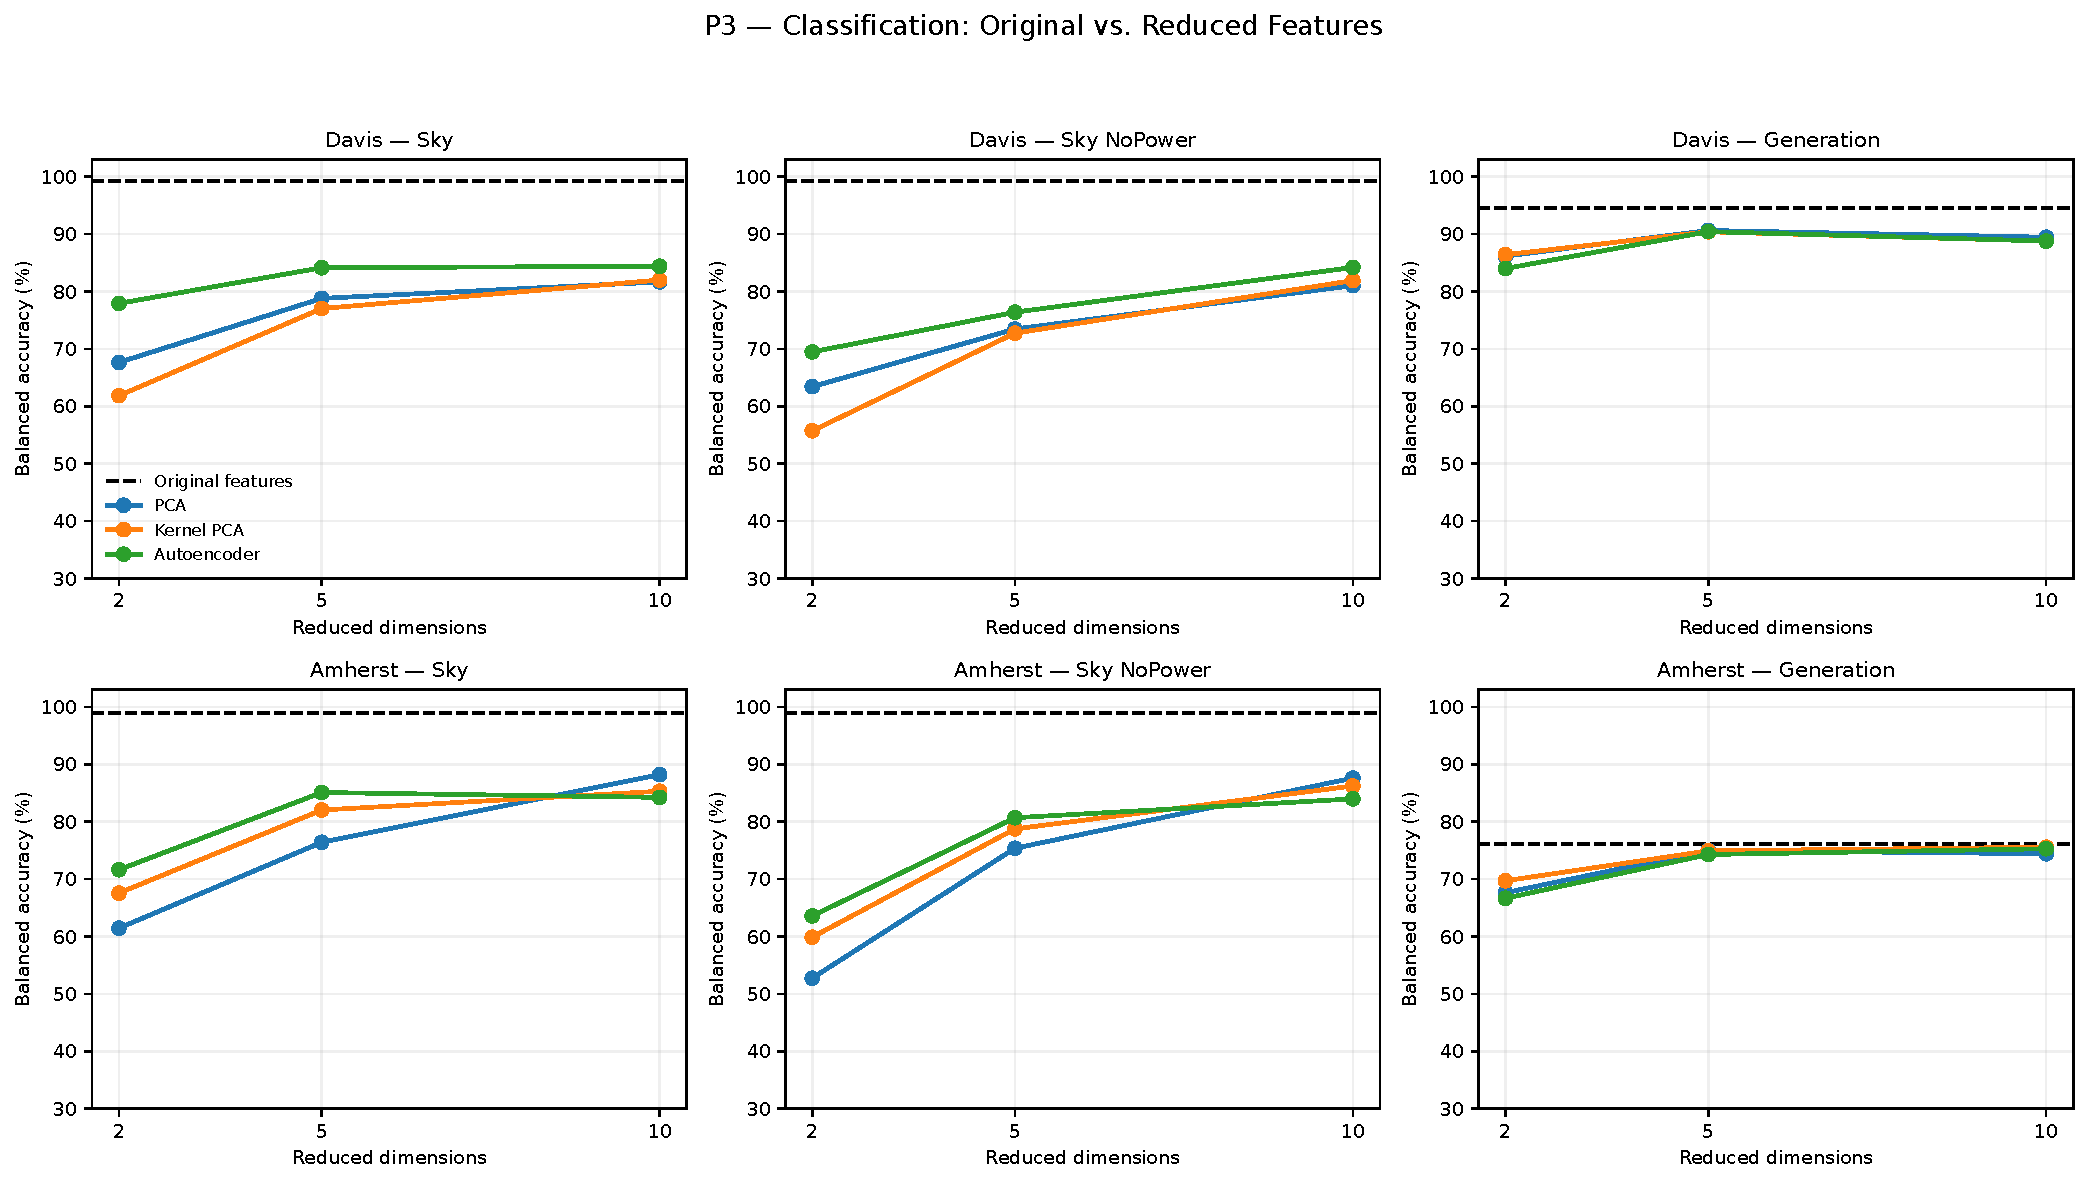
\includegraphics[width=0.94\textwidth]{Figures/P3/P3_Classification_All_Methods.pdf}
\caption{P3 classification balanced accuracy across reduced dimensions, contrasted with original features.}\label{fig:p3classcurve}
\end{figure}
\begin{figure}[!htbp]\centering
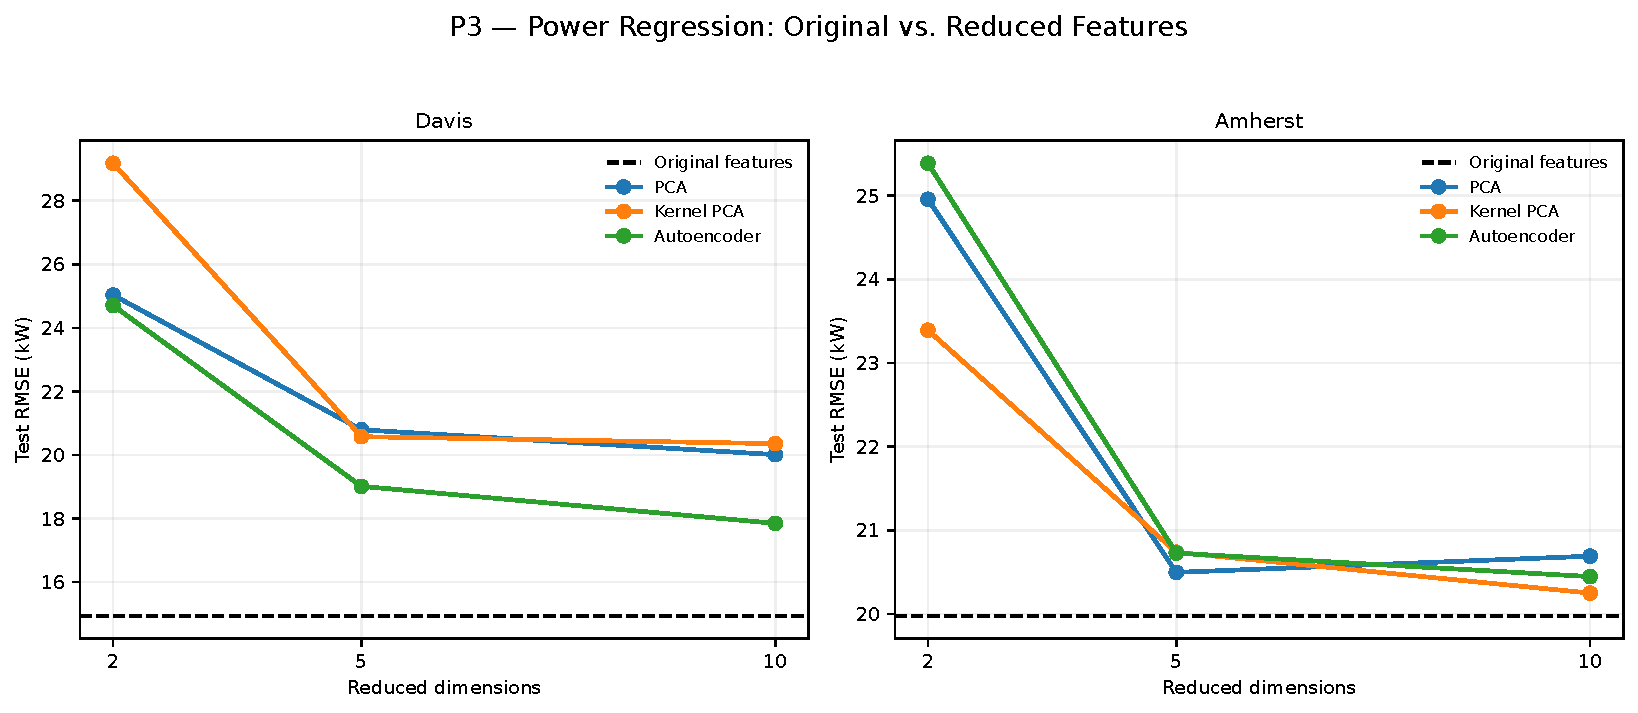
\includegraphics[width=0.85\textwidth]{Figures/P3/P3_Regression_All_Methods.pdf}
\caption{P3 power-regression RMSE across reduced dimensions, contrasted with original features.}\label{fig:p3regcurve}
\end{figure}
\begin{figure}[!htbp]\centering
\begin{subfigure}[b]{0.49\textwidth}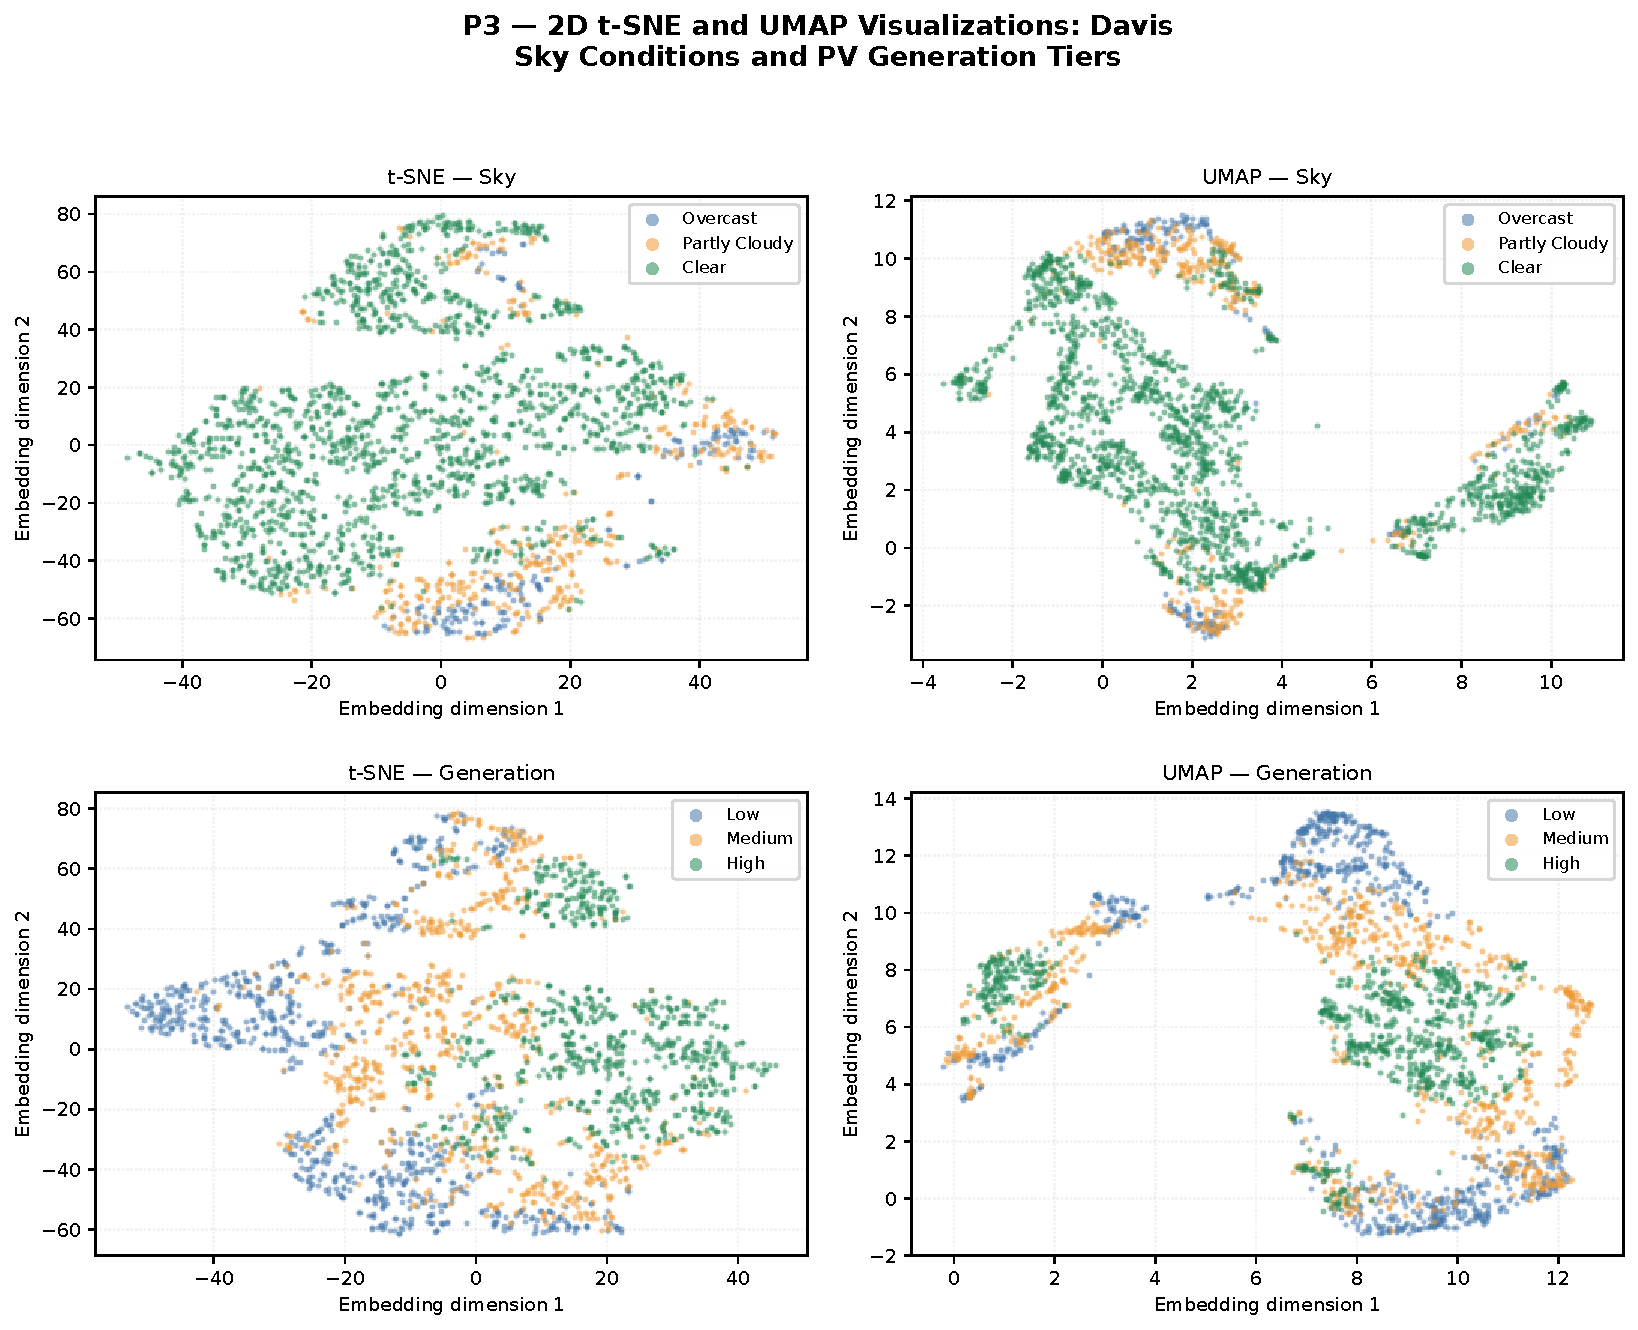
\includegraphics[width=\linewidth]{Figures/P3/P3_2D_tSNE_UMAP_Davis.pdf}\caption{Davis}\end{subfigure}\hfill
\begin{subfigure}[b]{0.49\textwidth}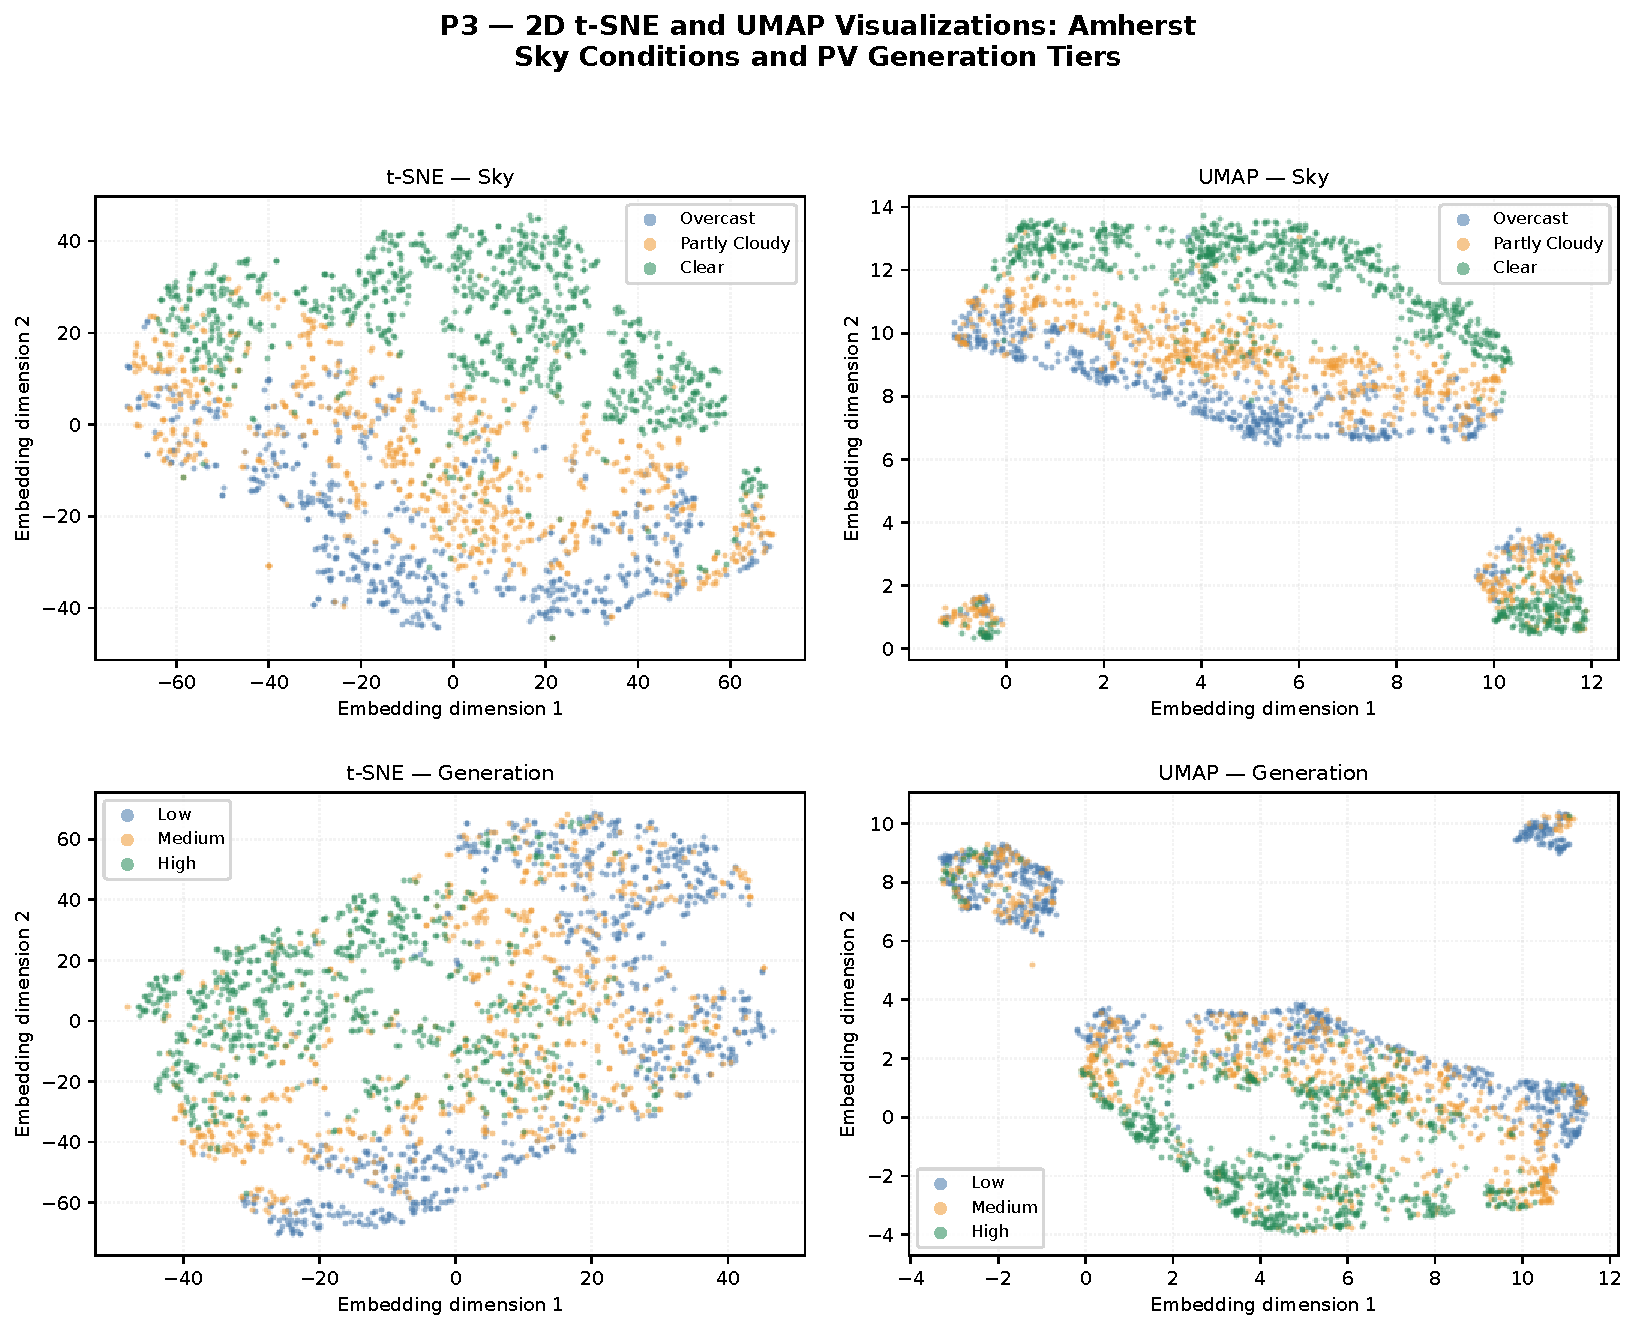
\includegraphics[width=\linewidth]{Figures/P3/P3_2D_tSNE_UMAP_Amherst.pdf}\caption{Amherst}\end{subfigure}
\caption{Training-set t-SNE and UMAP visualizations colored by sky-condition or generation class.}\label{fig:p3maps}
\end{figure}

\paragraph{Additional downstream metrics.}
Table~\ref{tab:p3acc} gives plain accuracy at $d=10$ for the BA-winning model of each
representation, and Tables~\ref{tab:p3mae} and~\ref{tab:p3nrmse} give MAE and nRMSE for the
RMSE-winning regressor. Using the primary-metric winner avoids choosing a separate test-set winner
for each metric. For complete MAE results at all three bottlenecks and for \emph{every}
regression model, Appendix~\ref{app:p3mae} compares the reduced representation with
that very same model on the original features.

\begin{table}[!htbp]\centering\footnotesize
\caption{P3 held-out classification accuracy at $d=10$ (\%), for the balanced-accuracy-winning model in each representation.}\label{tab:p3acc}
\begin{tabular}{@{}llrrrr@{}}\toprule
\textbf{City} & \textbf{Task} & \textbf{Original} & \textbf{PCA} & \textbf{Kernel PCA} & \textbf{AE}\\\midrule
Davis & Sky & 99.28 & 87.67 & 87.20 & 89.57\\
Davis & Sky\_NoPower & 99.29 & 87.42 & 87.70 & 89.67\\
Davis & Generation & 94.93 & 90.44 & 90.17 & 90.00\\
Amherst & Sky & 99.04 & 90.41 & 87.87 & 86.95\\
Amherst & Sky\_NoPower & 99.04 & 89.95 & 88.46 & 86.45\\
Amherst & Generation & 75.44 & 73.73 & 74.16 & 74.24\\
\bottomrule\end{tabular}
\end{table}
\begin{table}[!htbp]\centering\footnotesize
\begin{minipage}[t]{0.48\textwidth}\centering
\caption{P3 regression MAE (kW) at $d=10$.}\label{tab:p3mae}
\begin{tabular}{@{}lrrrr@{}}\toprule
\textbf{City} & \textbf{Orig.} & \textbf{PCA} & \textbf{KPCA} & \textbf{AE}\\\midrule
Davis & 8.71 & 12.46 & 13.84 & 11.20\\
Amherst & 13.50 & 14.44 & 14.68 & 14.40\\
\bottomrule\end{tabular}
\end{minipage}\hfill
\begin{minipage}[t]{0.48\textwidth}\centering
\caption{P3 regression nRMSE (\%) at $d=10$.}\label{tab:p3nrmse}
\begin{tabular}{@{}lrrrr@{}}\toprule
\textbf{City} & \textbf{Orig.} & \textbf{PCA} & \textbf{KPCA} & \textbf{AE}\\\midrule
Davis & 5.90 & 7.92 & 8.05 & 7.06\\
Amherst & 15.70 & 16.27 & 15.92 & 16.07\\
\bottomrule\end{tabular}
\end{minipage}
\end{table}

\subsection{Analysis and observations}
\paragraph{Unsupervised compression keeps variance, not label information.} PCA keeps the
directions of largest variance in the inputs. The sky label, however, is a \emph{ratio}
($\mathrm{GHI}/\mathrm{Clearsky\ GHI}$) that depends on a few irradiance columns, while much of the
input variance comes from temperature, humidity, pressure, wind and the time encodings. The label
signal is therefore spread thinly across components, which explains why sky classification loses
$11$--$15$ BA points even at $d=10$, and why two PCA components give only $47$--$53\%$ BA for
Amherst \texttt{Sky\_NoPower}.

\paragraph{Non-linear reducers help most when the bottleneck is tight.} At $d=2$ the autoencoder
is the best reducer for every sky task, and in Davis it gives the best compressed regression
($17.85$\,kW at $d=10$). Its seed variance is also the largest (SD up to $10.6$ points), because a
different local optimum is reached for each seed.

\paragraph{When compression is almost free.} Amherst generation and regression lose almost
nothing at $d=10$. Here the full-feature model is itself limited by information that is not in the
inputs (Section~\ref{sec:p1}), so removing redundant dimensions costs little.

\paragraph{Visual maps are not accuracy.} t-SNE and UMAP show clearly separated sky clusters and an
ordered Low$\to$Medium$\to$High gradient for generation, with Medium overlapping its neighbours.
These maps support the P1 analysis qualitatively but are not evidence of a better predictor.
\FloatBarrier

% =================================================================
\section{P4: Semi-Supervised Classification}\label{sec:p4}

\subsection{Objective and tasks}
P4 tests whether unlabeled observations improve the P1 sky and generation classifiers when only
$p\in\{10,30,50\}\%$ of training labels are revealed. The key quantity is the \emph{gain over a
matched supervised-only baseline} trained on exactly the same labeled subset, evaluated on the full
held-out test set.

\subsection{Preprocessing}
Only the training partition is divided into labeled and unlabeled subsets; the chronological test
set is unchanged. Each supervised-only baseline uses precisely the labeled samples available to
its SSL counterpart, and SSL methods may additionally use the remaining training inputs
\emph{without} labels. Label construction, encoding and thresholds follow the P1 rules. The test set
is never pseudo-labeled.

\subsection{Methods and models}
Four training strategies are applied to each of the five P1 classifiers: (i) supervised-only;
(ii) one-shot pseudo-labeling, in which the supervised model labels the unlabeled pool once and is
refitted on the union; (iii) iterative self-training, which repeats this and adds confident
pseudo-labels over several rounds; and (iv) autoencoder SSL, in which an autoencoder is trained on
\emph{all} training inputs (labeled and unlabeled) and the classifier is trained on its features
using the labeled subset. Figure~\ref{fig:p4flow} shows that supervised and SSL branches start from
the same label budget. Tables~\ref{tab:p4methods} and~\ref{tab:p4impl} list the methods.
\begin{table}[!htbp]\centering\footnotesize
\setlength{\tabcolsep}{5pt}
\caption{P4 model and method inventory, separating classical machine learning and deep learning.}\label{tab:p4methods}
\begin{tabular}{@{}p{0.19\linewidth}p{0.37\linewidth}p{0.34\linewidth}@{}}\toprule
\textbf{Family / stage} & \textbf{Models or strategies} & \textbf{Purpose}\\\midrule
\rowcolor{gold!10}
Classical ML & Logistic regression, RBF SVM & Supervised and pseudo-labeled fits\\
\rowcolor{gold!10}
Classical ML & Random forest, XGBoost & Supervised and pseudo-labeled fits\\
\rowcolor{teal!9}
Deep learning & PyTorch MLP & Neural classification\\
\rowcolor{teal!9}
Deep representation & Autoencoder SSL & Unsupervised feature learning\\
\rowcolor{mist}
SSL strategies & One-shot, iterative self-training & Compare with supervised-only baselines\\
\bottomrule\end{tabular}
\end{table}


\begin{table}[!htbp]\centering\footnotesize
\caption{P4 implementation families and fixed label-budget settings. Pseudo-label confidence rules, iteration caps, and neural optimizer settings should be transcribed from the executed P4 notebook.}\label{tab:p4impl}
\begin{tabularx}{\linewidth}{@{}p{0.24\linewidth}p{0.21\linewidth}X@{}}\toprule
\textbf{Method/family} & \textbf{Python library} & \textbf{Verified settings}\\\midrule
Classical classifiers & \texttt{scikit-learn}, \texttt{xgboost} & Logistic regression, RBF SVM, random forest, XGBoost.\\
Supervised / pseudo-label / iterative SSL & Python/scikit-learn orchestration & Matched label budgets of $10\%$, $30\%$, and $50\%$; remaining training examples have labels withheld.\\
Neural / autoencoder SSL & Neural implementation (confirm backend) & Autoencoder-based representation plus classifier; held-out test labels are never used for pseudo-label training.\\
\bottomrule\end{tabularx}
\end{table}


\begin{figure}[!htbp]\centering
\tikzfit{p4_ssl}
\caption{P4 matched semi-supervised evaluation. The labeled sample set is identical between supervised and SSL methods at each training-label budget.}\label{fig:p4flow}
\end{figure}

\subsection{Results}
Table~\ref{tab:p4} reports every classifier under all four strategies at each label budget, for
both cities and tasks. The highlighted cell in each city/task/budget group is the highest observed
mean balanced accuracy.

\begingroup
\scriptsize
\setlength{\tabcolsep}{3pt}
\begin{longtable}{@{}llr l rrrr@{}}
\caption{P4 complete classification results: every classifier and SSL strategy at 10\%, 30\%, and 50\% labeled training data (balanced accuracy, \%; mean $\pm$ SD, three seeds). Bold denotes the best combination within each city/task/budget.}\label{tab:p4}\\
\toprule
\textbf{City} & \textbf{Task} & \textbf{Labels} & \textbf{Classifier} & \textbf{Supervised} & \textbf{One-shot} & \textbf{Iterative} & \textbf{AE-SSL}\\\midrule
\endfirsthead
\multicolumn{8}{l}{\textit{P4 full comparison (continued)}}\\
\toprule
\textbf{City} & \textbf{Task} & \textbf{Labels} & \textbf{Classifier} & \textbf{Supervised} & \textbf{One-shot} & \textbf{Iterative} & \textbf{AE-SSL}\\\midrule
\endhead
\midrule\multicolumn{8}{r}{\footnotesize Continued on next page}\\
\endfoot
\bottomrule
\endlastfoot
Davis & Sky & 10\% & Logistic regression & 95.77\,$\pm$\,1.30 & 95.17\,$\pm$\,1.43 & 95.54\,$\pm$\,0.75 & 95.65\,$\pm$\,1.39\\
Davis & Sky & 10\% & RBF SVM & 91.73\,$\pm$\,0.89 & 90.78\,$\pm$\,0.63 & 91.30\,$\pm$\,0.89 & 91.69\,$\pm$\,1.22\\
Davis & Sky & 10\% & Random forest & 97.54\,$\pm$\,0.18 & 97.58\,$\pm$\,0.23 & 97.63\,$\pm$\,0.31 & 97.49\,$\pm$\,0.13\\
Davis & Sky & 10\% & XGBoost & \bestscore{97.92\,$\pm$\,0.38} & 97.67\,$\pm$\,0.30 & 97.72\,$\pm$\,0.31 & 97.86\,$\pm$\,0.40\\
Davis & Sky & 10\% & MLP (PyTorch) & 92.27\,$\pm$\,3.25 & 93.21\,$\pm$\,0.87 & 93.30\,$\pm$\,0.59 & 89.25\,$\pm$\,4.90\\
\addlinespace[3pt]
Davis & Sky & 30\% & Logistic regression & 98.37\,$\pm$\,0.26 & 98.45\,$\pm$\,0.22 & 98.43\,$\pm$\,0.23 & 98.31\,$\pm$\,0.41\\
Davis & Sky & 30\% & RBF SVM & 95.25\,$\pm$\,1.21 & 95.24\,$\pm$\,1.02 & 94.81\,$\pm$\,1.61 & 94.50\,$\pm$\,1.28\\
Davis & Sky & 30\% & Random forest & 98.46\,$\pm$\,0.03 & 98.59\,$\pm$\,0.12 & 98.33\,$\pm$\,0.26 & 98.26\,$\pm$\,0.20\\
Davis & Sky & 30\% & XGBoost & 98.72\,$\pm$\,0.31 & 98.28\,$\pm$\,0.34 & \bestscore{98.74\,$\pm$\,0.15} & 98.53\,$\pm$\,0.30\\
Davis & Sky & 30\% & MLP (PyTorch) & 97.18\,$\pm$\,0.66 & 97.33\,$\pm$\,0.49 & 97.26\,$\pm$\,0.92 & 96.16\,$\pm$\,1.54\\
\addlinespace[3pt]
Davis & Sky & 50\% & Logistic regression & 98.39\,$\pm$\,0.30 & 98.42\,$\pm$\,0.27 & 98.36\,$\pm$\,0.27 & 98.46\,$\pm$\,0.22\\
Davis & Sky & 50\% & RBF SVM & 96.16\,$\pm$\,0.74 & 96.35\,$\pm$\,1.26 & 96.31\,$\pm$\,0.99 & 95.65\,$\pm$\,1.59\\
Davis & Sky & 50\% & Random forest & 98.62\,$\pm$\,0.14 & 98.59\,$\pm$\,0.12 & 98.54\,$\pm$\,0.18 & 98.44\,$\pm$\,0.05\\
Davis & Sky & 50\% & XGBoost & \bestscore{99.14\,$\pm$\,0.18} & 99.07\,$\pm$\,0.20 & 99.03\,$\pm$\,0.06 & 98.91\,$\pm$\,0.27\\
Davis & Sky & 50\% & MLP (PyTorch) & 97.58\,$\pm$\,0.42 & 97.95\,$\pm$\,0.12 & 98.17\,$\pm$\,0.52 & 97.46\,$\pm$\,0.25\\
\addlinespace[3pt]
Davis & Generation & 10\% & Logistic regression & 92.10\,$\pm$\,1.41 & 88.44\,$\pm$\,0.42 & 91.90\,$\pm$\,1.30 & 91.77\,$\pm$\,1.38\\
Davis & Generation & 10\% & RBF SVM & 91.03\,$\pm$\,0.50 & 90.74\,$\pm$\,0.74 & 91.11\,$\pm$\,0.38 & 90.85\,$\pm$\,0.83\\
Davis & Generation & 10\% & Random forest & 94.39\,$\pm$\,0.29 & 94.29\,$\pm$\,0.24 & 94.38\,$\pm$\,0.33 & 94.20\,$\pm$\,0.33\\
Davis & Generation & 10\% & XGBoost & 94.63\,$\pm$\,0.25 & \bestscore{94.71\,$\pm$\,0.28} & 94.67\,$\pm$\,0.31 & 94.39\,$\pm$\,0.26\\
Davis & Generation & 10\% & MLP (PyTorch) & 85.55\,$\pm$\,10.16 & 86.00\,$\pm$\,10.46 & 86.01\,$\pm$\,10.46 & 91.14\,$\pm$\,1.48\\
\addlinespace[3pt]
Davis & Generation & 30\% & Logistic regression & 93.98\,$\pm$\,0.44 & 93.77\,$\pm$\,0.11 & 93.71\,$\pm$\,0.27 & 93.86\,$\pm$\,0.45\\
Davis & Generation & 30\% & RBF SVM & 93.46\,$\pm$\,0.23 & 93.47\,$\pm$\,0.30 & 93.50\,$\pm$\,0.38 & 92.94\,$\pm$\,0.85\\
Davis & Generation & 30\% & Random forest & 94.90\,$\pm$\,0.14 & 94.91\,$\pm$\,0.23 & 94.93\,$\pm$\,0.03 & 94.71\,$\pm$\,0.30\\
Davis & Generation & 30\% & XGBoost & \bestscore{95.49\,$\pm$\,0.42} & 95.39\,$\pm$\,0.48 & 95.43\,$\pm$\,0.30 & 95.42\,$\pm$\,0.19\\
Davis & Generation & 30\% & MLP (PyTorch) & 93.43\,$\pm$\,1.16 & 94.05\,$\pm$\,0.92 & 94.45\,$\pm$\,0.71 & 94.09\,$\pm$\,0.62\\
\addlinespace[3pt]
Davis & Generation & 50\% & Logistic regression & 94.41\,$\pm$\,0.29 & 94.49\,$\pm$\,0.40 & 94.46\,$\pm$\,0.41 & 93.96\,$\pm$\,0.21\\
Davis & Generation & 50\% & RBF SVM & 94.15\,$\pm$\,0.32 & 94.01\,$\pm$\,0.28 & 94.05\,$\pm$\,0.31 & 93.88\,$\pm$\,0.54\\
Davis & Generation & 50\% & Random forest & 95.39\,$\pm$\,0.23 & 95.34\,$\pm$\,0.13 & 95.39\,$\pm$\,0.16 & 95.09\,$\pm$\,0.35\\
Davis & Generation & 50\% & XGBoost & \bestscore{95.92\,$\pm$\,0.30} & 95.90\,$\pm$\,0.05 & 95.85\,$\pm$\,0.09 & 95.87\,$\pm$\,0.10\\
Davis & Generation & 50\% & MLP (PyTorch) & 94.14\,$\pm$\,0.68 & 94.16\,$\pm$\,0.97 & 94.44\,$\pm$\,0.46 & 94.23\,$\pm$\,0.37\\
\addlinespace[3pt]
Amherst & Sky & 10\% & Logistic regression & 97.06\,$\pm$\,0.69 & 96.94\,$\pm$\,0.32 & 97.05\,$\pm$\,0.56 & 96.79\,$\pm$\,0.57\\
Amherst & Sky & 10\% & RBF SVM & 92.76\,$\pm$\,2.11 & 92.41\,$\pm$\,2.35 & 92.44\,$\pm$\,2.08 & 92.82\,$\pm$\,1.13\\
Amherst & Sky & 10\% & Random forest & 97.65\,$\pm$\,0.52 & 97.65\,$\pm$\,0.65 & 97.60\,$\pm$\,0.60 & 97.55\,$\pm$\,0.52\\
Amherst & Sky & 10\% & XGBoost & 97.79\,$\pm$\,0.66 & \bestscore{97.88\,$\pm$\,0.57} & 97.79\,$\pm$\,0.65 & 97.81\,$\pm$\,0.47\\
Amherst & Sky & 10\% & MLP (PyTorch) & 95.68\,$\pm$\,1.55 & 96.11\,$\pm$\,0.56 & 96.22\,$\pm$\,0.74 & 95.82\,$\pm$\,0.03\\
\addlinespace[3pt]
Amherst & Sky & 30\% & Logistic regression & 97.68\,$\pm$\,0.45 & 97.74\,$\pm$\,0.47 & 97.71\,$\pm$\,0.44 & 97.43\,$\pm$\,0.41\\
Amherst & Sky & 30\% & RBF SVM & 94.76\,$\pm$\,0.48 & 94.84\,$\pm$\,0.70 & 94.64\,$\pm$\,0.51 & 94.44\,$\pm$\,0.20\\
Amherst & Sky & 30\% & Random forest & 98.23\,$\pm$\,0.23 & 98.17\,$\pm$\,0.22 & 98.22\,$\pm$\,0.15 & 98.19\,$\pm$\,0.19\\
Amherst & Sky & 30\% & XGBoost & 98.36\,$\pm$\,0.33 & 98.46\,$\pm$\,0.29 & \bestscore{98.47\,$\pm$\,0.29} & 98.36\,$\pm$\,0.27\\
Amherst & Sky & 30\% & MLP (PyTorch) & 96.16\,$\pm$\,0.65 & 96.72\,$\pm$\,0.19 & 96.51\,$\pm$\,0.68 & 96.01\,$\pm$\,0.95\\
\addlinespace[3pt]
Amherst & Sky & 50\% & Logistic regression & 97.92\,$\pm$\,0.55 & 97.92\,$\pm$\,0.55 & 97.90\,$\pm$\,0.52 & 97.66\,$\pm$\,0.54\\
Amherst & Sky & 50\% & RBF SVM & 95.42\,$\pm$\,0.53 & 95.33\,$\pm$\,0.81 & 95.18\,$\pm$\,0.49 & 95.31\,$\pm$\,0.64\\
Amherst & Sky & 50\% & Random forest & 98.61\,$\pm$\,0.07 & 98.53\,$\pm$\,0.08 & 98.55\,$\pm$\,0.11 & 98.59\,$\pm$\,0.13\\
Amherst & Sky & 50\% & XGBoost & 98.72\,$\pm$\,0.21 & 98.72\,$\pm$\,0.18 & \bestscore{98.77\,$\pm$\,0.12} & 98.74\,$\pm$\,0.24\\
Amherst & Sky & 50\% & MLP (PyTorch) & 96.75\,$\pm$\,0.17 & 96.85\,$\pm$\,0.34 & 97.27\,$\pm$\,0.41 & 96.74\,$\pm$\,0.80\\
\addlinespace[3pt]
Amherst & Generation & 10\% & Logistic regression & 73.48\,$\pm$\,1.07 & 69.43\,$\pm$\,1.40 & 71.13\,$\pm$\,1.84 & 73.84\,$\pm$\,0.68\\
Amherst & Generation & 10\% & RBF SVM & 69.99\,$\pm$\,0.81 & 69.89\,$\pm$\,0.63 & 70.03\,$\pm$\,0.26 & 69.94\,$\pm$\,0.98\\
Amherst & Generation & 10\% & Random forest & 74.46\,$\pm$\,0.56 & 74.36\,$\pm$\,0.85 & \bestscore{74.62\,$\pm$\,0.70} & 74.58\,$\pm$\,0.99\\
Amherst & Generation & 10\% & XGBoost & 74.09\,$\pm$\,0.60 & 74.00\,$\pm$\,0.66 & 74.33\,$\pm$\,0.68 & 73.88\,$\pm$\,0.19\\
Amherst & Generation & 10\% & MLP (PyTorch) & 74.02\,$\pm$\,1.26 & 74.05\,$\pm$\,1.20 & 73.93\,$\pm$\,1.85 & 73.73\,$\pm$\,1.06\\
\addlinespace[3pt]
Amherst & Generation & 30\% & Logistic regression & 74.30\,$\pm$\,0.50 & 73.19\,$\pm$\,0.66 & 73.77\,$\pm$\,0.68 & 74.17\,$\pm$\,0.56\\
Amherst & Generation & 30\% & RBF SVM & 71.14\,$\pm$\,1.31 & 71.06\,$\pm$\,0.65 & 70.99\,$\pm$\,0.82 & 71.25\,$\pm$\,1.23\\
Amherst & Generation & 30\% & Random forest & 75.03\,$\pm$\,0.26 & 75.03\,$\pm$\,0.18 & 75.16\,$\pm$\,0.25 & \bestscore{75.23\,$\pm$\,0.54}\\
Amherst & Generation & 30\% & XGBoost & 74.75\,$\pm$\,0.84 & 75.08\,$\pm$\,0.51 & 75.05\,$\pm$\,0.80 & 74.86\,$\pm$\,0.81\\
Amherst & Generation & 30\% & MLP (PyTorch) & 74.41\,$\pm$\,0.95 & 74.41\,$\pm$\,0.77 & 74.29\,$\pm$\,0.94 & 74.56\,$\pm$\,0.20\\
\addlinespace[3pt]
Amherst & Generation & 50\% & Logistic regression & 74.40\,$\pm$\,0.33 & 73.56\,$\pm$\,0.12 & 73.91\,$\pm$\,0.23 & 74.09\,$\pm$\,0.53\\
Amherst & Generation & 50\% & RBF SVM & 72.05\,$\pm$\,1.26 & 71.73\,$\pm$\,1.40 & 71.83\,$\pm$\,1.20 & 71.82\,$\pm$\,1.31\\
Amherst & Generation & 50\% & Random forest & 75.18\,$\pm$\,0.41 & 75.36\,$\pm$\,0.28 & 75.36\,$\pm$\,0.23 & \bestscore{75.59\,$\pm$\,0.49}\\
Amherst & Generation & 50\% & XGBoost & 75.29\,$\pm$\,0.48 & 75.45\,$\pm$\,0.04 & 75.32\,$\pm$\,0.46 & 75.40\,$\pm$\,0.63\\
Amherst & Generation & 50\% & MLP (PyTorch) & 74.41\,$\pm$\,1.05 & 74.44\,$\pm$\,1.15 & 73.97\,$\pm$\,0.67 & 74.62\,$\pm$\,0.16\\
\addlinespace[3pt]
\end{longtable}
\endgroup


\paragraph{Can SSL beat the supervised baseline at 10\% labels?}
The specification asks this question explicitly. Table~\ref{tab:p4gain} answers it in two ways:
best-vs-best (does the best SSL configuration beat the best supervised configuration?) and matched
(for the same classifier, how much does the best SSL strategy add?). Values are computed from the
three-seed means in Table~\ref{tab:p4}.

\begin{table}[!htbp]\centering\footnotesize
\caption{P4 answer at 10\% labels (balanced accuracy, \%). ``Gain'' = SSL $-$ supervised; positive means unlabeled data helped. The last column counts positive matched gains over the 15 classifier/strategy pairs.}\label{tab:p4gain}
\setlength{\tabcolsep}{4pt}
\begin{tabular}{@{}llrlrr lr r@{}}\toprule
 & & \multicolumn{2}{c}{\textbf{Best supervised}} & \multicolumn{3}{c}{\textbf{Best SSL}} & \textbf{Largest matched} & \textbf{Pairs}\\
\cmidrule(lr){3-4}\cmidrule(lr){5-7}
\textbf{City} & \textbf{Task} & \textbf{BA} & \textbf{Model} & \textbf{BA} & \textbf{Config.} & \textbf{Gain} & \textbf{gain (config.)} & \textbf{$>0$}\\\midrule
Davis & Sky & 97.92 & XGB & 97.86 & XGB+AE & $-0.06$ & $+1.03$ (MLP+Iter.) & 4/15\\
Davis & Generation & 94.63 & XGB & 94.71 & XGB+One-shot & \textbf{$+0.08$} & $+5.59$ (MLP+AE) & 6/15\\
Amherst & Sky & 97.79 & XGB & 97.88 & XGB+One-shot & \textbf{$+0.09$} & $+0.54$ (MLP+Iter.) & 6/15\\
Amherst & Generation & 74.46 & RF & 74.62 & RF+Iter. & \textbf{$+0.16$} & $+0.36$ (LR+AE) & 6/15\\
\bottomrule\end{tabular}
\end{table}

So the answer is \emph{yes, but only marginally}: in three of four tasks the best SSL configuration
beats the best supervised one at 10\% labels, by $0.08$--$0.16$ points, which is smaller than the
seed SD of most entries. The only large matched gain is the MLP with autoencoder SSL on Davis
generation ($+5.59$ points, $85.55\to91.14\%$); its gain SD of $8.80$ points across seeds means the
improvement is real on average but not reliable for any single run.

Figure~\ref{fig:p4efficiency} shows the best-observed label-efficiency curves, and
Figure~\ref{fig:p4davisdetail} separates each classifier on Davis generation so that every SSL
curve can be compared with \emph{its own} supervised baseline.

\fign{Figures/P4/P4_Best_Observed_Label_Efficiency_Overview.pdf}{P4 best observed label-efficiency curves (balanced accuracy) across Davis and Amherst classification tasks.}{fig:p4efficiency}
\fign{Figures/P4/P4_Davis_Generation_Balanced_Accuracy_All_Models.pdf}{Per-classifier label-efficiency curves on Davis generation classification, with matched supervised baselines.}{fig:p4davisdetail}

\paragraph{Macro-F1 curves and area under the curve.}
The specification asks for label-efficiency curves in macro-F1.
Figure~\ref{fig:p4f1} shows them for generation classification in both cities, and
Table~\ref{tab:p4auc} summarizes the balanced-accuracy curve of XGBoost by its normalized area
under the curve from 10\% to 50\% labels. All AUC differences are within one SD.
\begin{figure}[!htbp]\centering
\begin{subfigure}[b]{0.49\textwidth}
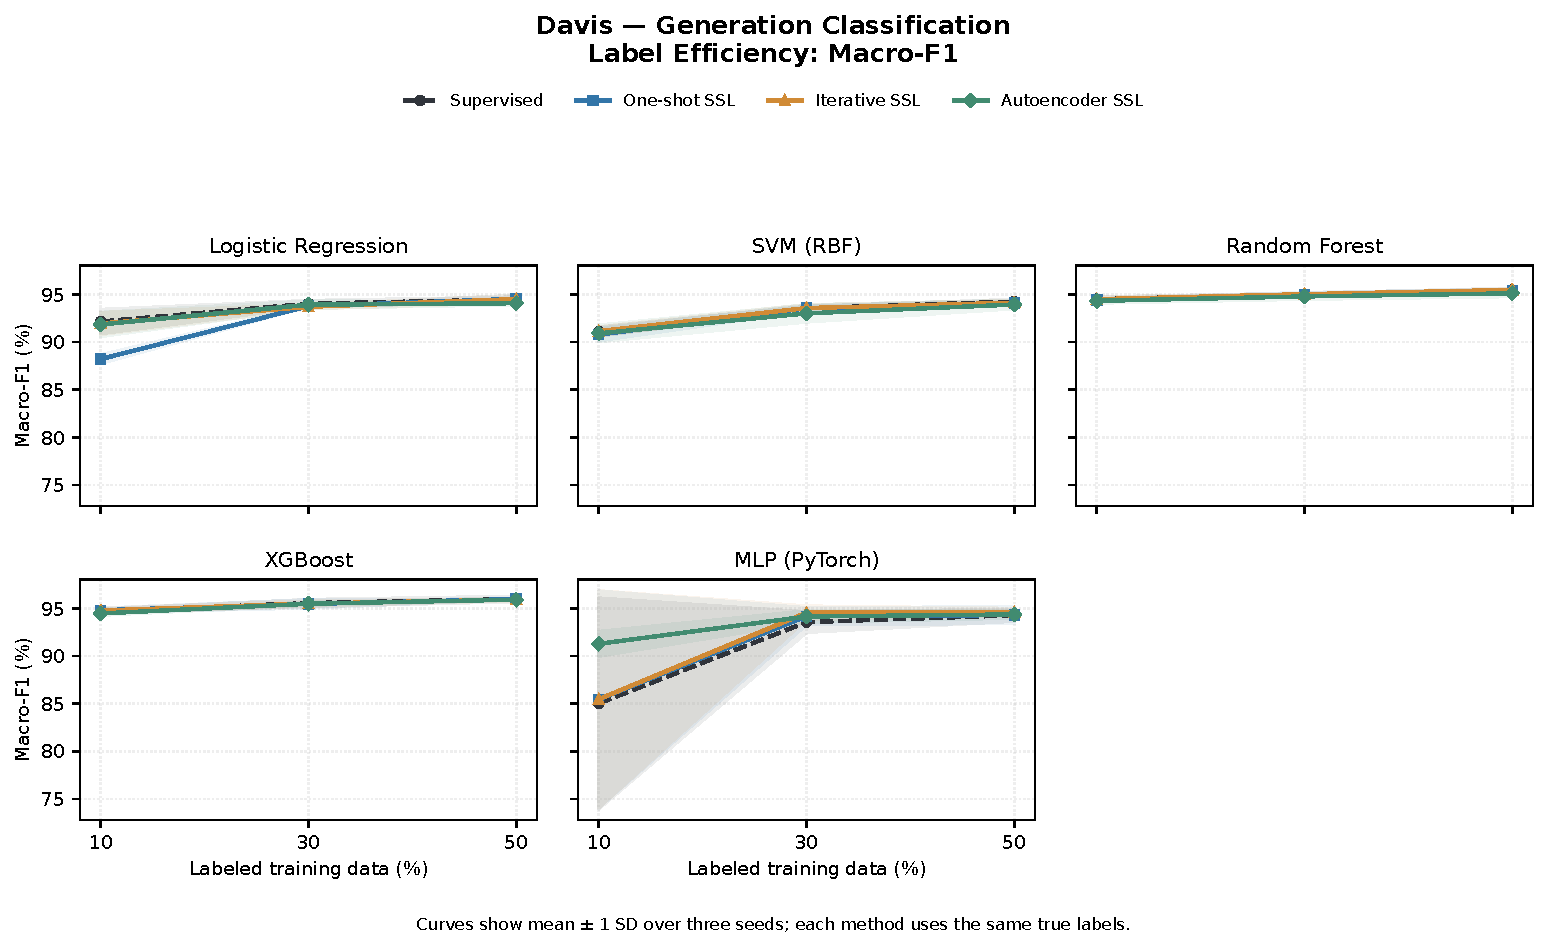
\includegraphics[width=\linewidth]{Figures/P4/P4_Davis_Generation_Macro_F1_All_Models.pdf}
\caption{Davis generation}
\end{subfigure}\hfill
\begin{subfigure}[b]{0.49\textwidth}
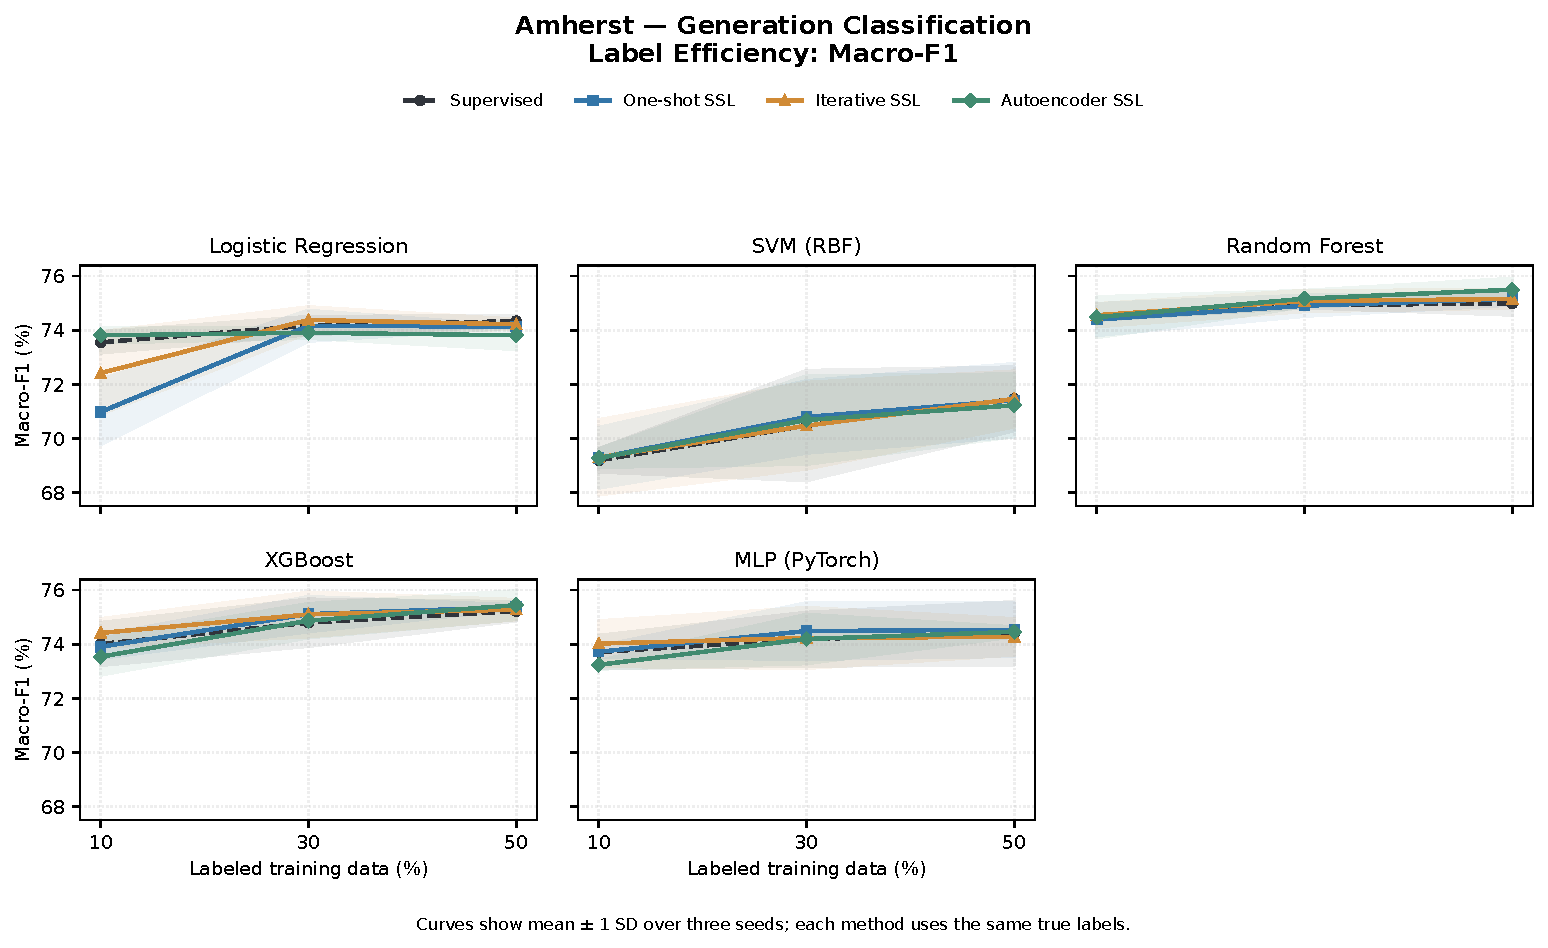
\includegraphics[width=\linewidth]{Figures/P4/P4_Amherst_Generation_Macro_F1_All_Models.pdf}
\caption{Amherst generation}
\end{subfigure}
\caption{P4 macro-F1 versus labeled training fraction for supervised-only
and semi-supervised classifiers on the same full held-out test set.}
\label{fig:p4f1}
\end{figure}

\begin{table}[!htbp]\centering\scriptsize
\setlength{\tabcolsep}{3pt}
\caption{P4 normalized label-efficiency AUC for XGBoost (three-seed mean $\pm$ SD), balanced-accuracy curve from 10\% to 50\% labels.}\label{tab:p4auc}
\begin{tabular}{@{}llrrrr@{}}\toprule
\textbf{City} & \textbf{Task} & \textbf{Supervised} & \textbf{One-shot} & \textbf{Iterative} & \textbf{AE SSL}\\\midrule
Davis & Sky & 0.986\,$\pm$\,0.003 & 0.983\,$\pm$\,0.003 & 0.986\,$\pm$\,0.000 & 0.985\,$\pm$\,0.003\\
Davis & Generation & 0.954\,$\pm$\,0.003 & 0.953\,$\pm$\,0.003 & 0.953\,$\pm$\,0.002 & 0.953\,$\pm$\,0.001\\
Amherst & Sky & 0.983\,$\pm$\,0.003 & 0.984\,$\pm$\,0.003 & 0.984\,$\pm$\,0.003 & 0.983\,$\pm$\,0.003\\
Amherst & Generation & 0.747\,$\pm$\,0.004 & 0.749\,$\pm$\,0.001 & 0.749\,$\pm$\,0.003 & 0.748\,$\pm$\,0.006\\
\bottomrule\end{tabular}
\end{table}

\subsection{Analysis and observations}
\paragraph{Why the gains are small.} Two effects limit SSL here. First, the supervised baselines are
already near their ceiling: even 10\% of a multi-year training partition is on the order of a
thousand labeled observations, and XGBoost loses only about $1$ BA point between 50\% and 10\%
labels. Second, pseudo-labeling can only reinforce what the supervised model already predicts; on
the hardest class (Amherst Medium) its own errors are recycled as labels, which is why one-shot
pseudo-labeling \emph{lowers} logistic regression by $4$ points on Amherst generation.

\paragraph{Who benefits.} The data-hungry, high-variance learner benefits most: at 10\% labels
the supervised MLP has an SD of $10.2$ points on Davis generation, and autoencoder features
learned from all training inputs stabilize it (SD $1.5$). Low-variance learners (XGBoost, RF) gain
almost nothing. The value of unlabeled data is therefore method- and budget-dependent, and SSL
is most useful as a variance reducer for neural models at the smallest label budgets.
\FloatBarrier

% =================================================================
\section{P5: Cross-City Transfer Learning}\label{sec:p5}

\subsection{Objective and tasks}
P5 asks whether the data-rich Davis source (six years) can improve power regression in the
label-scarce Amherst target, given $k\in\{10,50,100\}$ labeled target observations. Three families are
compared on the same held-out Amherst test set: source-only \emph{zero-shot} prediction;
\emph{target-only few-shot} training on the $k$ labels; and \emph{transfer} methods that adapt a
source model or combine source and target data. The goal set by the specification is a transfer
method that beats both baselines.

\subsection{Preprocessing}
Source and target data remain geographically separate. Source models are fitted on Davis
training data; the $k$ target examples come only from Amherst's training portion; and every
adaptation step uses only those $k$ labels. Amherst test labels are used solely for final scoring,
for every budget and seed.

\subsection{Methods and models}
Four transfer strategies are evaluated (Figure~\ref{fig:p5flow}):
\begin{itemize}[leftmargin=1.5em,itemsep=2pt]
\item \textbf{Affine calibration:} keep the Davis model and fit a scale and offset on the $k$ target
labels, $\hat y_{\mathrm{Amherst}} = a\,\hat y_{\mathrm{Davis}}(x) + b$. This corrects the systematic
scale bias seen in P2 without retraining the predictor.
\item \textbf{Joint calibrated pooling:} rescale the Davis training targets to Amherst's output
scale using the $k$ labels, then fit one model on the calibrated Davis data together with the $k$
Amherst samples. The model borrows Davis's many weather situations while respecting Amherst's
power level.
\item \textbf{Frozen encoder + Ridge (neural):} reuse the hidden layers of a Davis-trained MLP as a
fixed feature extractor and fit a new Ridge output layer on the $k$ Amherst labels.
\item \textbf{Partial fine-tuning (neural):} start from the Davis-pretrained MLP, freeze the early
layers and update the later layers on the $k$ Amherst labels.
\end{itemize}
Restricting what is learned from 10--100 target labels limits overfitting. Ridge, random forest,
XGBoost and the MLP serve as base models (Tables~\ref{tab:p5methods} and~\ref{tab:p5impl}).
\begin{table}[!htbp]\centering\footnotesize
\setlength{\tabcolsep}{5pt}
\caption{P5 model and method inventory, separating classical machine learning and deep learning.}\label{tab:p5methods}
\begin{tabular}{@{}p{0.19\linewidth}p{0.37\linewidth}p{0.34\linewidth}@{}}\toprule
\textbf{Family / stage} & \textbf{Models or strategies} & \textbf{Purpose}\\\midrule
\rowcolor{gold!10}
Classical ML & Ridge, random forest, XGBoost & Target-only and transfer baselines\\
\rowcolor{gold!10}
Classical transfer & Affine calibration; joint pooling & Adapt predictions/source-target data\\
\rowcolor{teal!9}
Deep learning & PyTorch MLP & Neural target/source regression\\
\rowcolor{teal!9}
Neural transfer & Frozen encoder + ridge; partial fine-tuning & Transfer neural representations\\
\bottomrule\end{tabular}
\end{table}


\begin{table}[!htbp]\centering\footnotesize
\caption{P5 libraries and verified transfer protocol. Model-specific learning rates, regularization strengths, and optimizer schedules require checking against the executed P5 notebook.}\label{tab:p5impl}
\begin{tabularx}{\linewidth}{@{}p{0.24\linewidth}p{0.21\linewidth}X@{}}\toprule
\textbf{Model/strategy} & \textbf{Python library} & \textbf{Verified settings}\\\midrule
Source/target classical models & \texttt{scikit-learn}, \texttt{xgboost} & Ridge, random forest, XGBoost; source Davis 2011--2016, target Amherst 2018--2020.\\
Calibration and source--target pooling & NumPy / classical estimators & Affine prediction calibration and joint calibrated pooling on the $k$ labeled target examples.\\
Neural transfer & \texttt{PyTorch}; \texttt{scikit-learn} ridge & MLP, frozen-encoder features, ridge prediction, and partial fine-tuning.\\
Target-label budgets & Experiment protocol & $k\in\{10,50,100\}$ labels; three seeds, held-out Amherst test evaluation.\\
\bottomrule\end{tabularx}
\end{table}


\begin{figure}[!htbp]\centering
\tikzfit{p5_transfer}
\caption{P5 transfer experiment, contrasting source-only, target-only, and adapted models on a held-out Amherst test set.}\label{fig:p5flow}
\end{figure}

\subsection{Results}
Table~\ref{tab:p5zeroshot} reports the four zero-shot source models; the best (Ridge) still has
$75.82$\,kW RMSE ($59.6\%$ nRMSE). Table~\ref{tab:p5} compares every target-only and transfer
strategy at each label budget.

\begin{table}[!htbp]\centering\footnotesize
\setlength{\tabcolsep}{5pt}
\caption{P5 direct Davis-to-Amherst zero-shot performance for all four models (mean $\pm$ SD, kW).}\label{tab:p5zeroshot}
\begin{tabular}{@{}lrr@{}}\toprule
\textbf{Source model} & \textbf{Zero-shot RMSE} & \textbf{Zero-shot MAE}\\\midrule
Ridge & \bestscore{75.82\,$\pm$\,0.00} & 61.24\,$\pm$\,0.00\\
Random forest & 77.72\,$\pm$\,0.04 & 64.04\,$\pm$\,0.09\\
XGBoost & 77.98\,$\pm$\,0.13 & 63.38\,$\pm$\,0.19\\
MLP (PyTorch) & 83.24\,$\pm$\,7.84 & 69.16\,$\pm$\,5.10\\
\bottomrule\end{tabular}
\end{table}

\begin{table}[!htbp]\centering\scriptsize
\setlength{\tabcolsep}{3pt}
\caption{P5 all evaluated target-only and transfer settings (held-out Amherst RMSE in kW, mean $\pm$ SD). Bold marks the best configuration at each label budget.}\label{tab:p5}
\begin{tabular}{@{}l l rrr@{}}\toprule
\textbf{Base model} & \textbf{Training / adaptation strategy} & \textbf{$k=10$} & \textbf{$k=50$} & \textbf{$k=100$}\\\midrule
Ridge & Target-Only & 26.19\,$\pm$\,1.99 & \bestscore{22.03\,$\pm$\,0.53} & 22.09\,$\pm$\,0.63\\
Ridge & Affine Calibration & 24.52\,$\pm$\,1.92 & 22.96\,$\pm$\,0.39 & 22.67\,$\pm$\,0.05\\
Ridge & Joint Calibrated Pooling & \bestscore{23.22\,$\pm$\,0.66} & 22.03\,$\pm$\,0.58 & 21.81\,$\pm$\,0.47\\
Random forest & Target-Only & 30.60\,$\pm$\,5.42 & 22.69\,$\pm$\,0.37 & 22.04\,$\pm$\,0.62\\
Random forest & Affine Calibration & 24.92\,$\pm$\,2.17 & 22.92\,$\pm$\,0.42 & 22.91\,$\pm$\,0.15\\
Random forest & Joint Calibrated Pooling & 25.12\,$\pm$\,2.44 & 22.29\,$\pm$\,0.71 & \bestscore{21.80\,$\pm$\,0.42}\\
XGBoost & Target-Only & 31.15\,$\pm$\,4.79 & 24.90\,$\pm$\,1.12 & 23.07\,$\pm$\,0.46\\
XGBoost & Affine Calibration & 24.30\,$\pm$\,1.62 & 22.68\,$\pm$\,0.32 & 22.60\,$\pm$\,0.09\\
XGBoost & Joint Calibrated Pooling & 24.87\,$\pm$\,2.26 & 22.60\,$\pm$\,0.30 & 22.29\,$\pm$\,0.53\\
MLP (PyTorch) & Target-Only & 29.31\,$\pm$\,2.97 & 23.94\,$\pm$\,0.67 & 24.24\,$\pm$\,0.35\\
MLP (PyTorch) & Affine Calibration & 26.91\,$\pm$\,5.39 & 26.80\,$\pm$\,7.22 & 25.44\,$\pm$\,4.92\\
MLP (PyTorch) & Frozen Encoder + Ridge & 27.12\,$\pm$\,2.44 & 25.64\,$\pm$\,0.65 & 24.20\,$\pm$\,0.42\\
MLP (PyTorch) & Partial Fine-Tuning & 24.33\,$\pm$\,2.13 & 23.03\,$\pm$\,1.63 & 22.21\,$\pm$\,0.23\\
\bottomrule\end{tabular}
\end{table}



\paragraph{Required comparison: zero-shot vs few-shot vs transfer.}
Table~\ref{tab:p5consolidated} puts the best zero-shot, best target-only and best transfer result
side by side for each budget. Gain is oriented so that positive means transfer helped.

\begin{table}[!htbp]\centering\footnotesize
\caption{P5 consolidated held-out Amherst comparison: RMSE (kW) / nRMSE (\%), best observed three-seed mean per approach. Gain = target-only $-$ transfer RMSE.}\label{tab:p5consolidated}
\setlength{\tabcolsep}{5pt}
\begin{tabular}{@{}rllll@{}}\toprule
\textbf{$k$} & \textbf{Zero-shot} & \textbf{Target-only} & \textbf{Transfer} & \textbf{Gain (kW)}\\\midrule
10 & 75.82 / 59.61 (Ridge) & 26.19 / 20.59 (Ridge) & \bestscore{23.22 / 18.26} (Pooling, Ridge) & $+2.97$\\
50 & 75.82 / 59.61 (Ridge) & 22.03 / 17.32 (Ridge) & 22.03 / 17.32 (Pooling, Ridge) & $+0.00$\\
100 & 75.82 / 59.61 (Ridge) & 22.04 / 17.33 (RF) & 21.80 / 17.14 (Pooling, RF) & $+0.24$\\
\bottomrule\end{tabular}
\end{table}

\paragraph{Matched transfer gain per base model.}
Best-vs-best hides how much each model gains from the source. Table~\ref{tab:p5matched} gives
the matched gain (target-only RMSE minus transfer RMSE for the \emph{same} base model and budget),
computed from Table~\ref{tab:p5}.

\begin{table}[!htbp]\centering\footnotesize
\caption{P5 matched transfer gain (kW) = target-only RMSE $-$ transfer RMSE for the same base model and $k$. Positive = transfer helped; negative = negative transfer (shaded).}\label{tab:p5matched}
\setlength{\tabcolsep}{6pt}
\begin{tabular}{@{}llrrr@{}}\toprule
\textbf{Base model} & \textbf{Strategy} & \textbf{$k=10$} & \textbf{$k=50$} & \textbf{$k=100$}\\\midrule
Ridge & Affine calibration & $+1.67$ & \cellcolor{gold!17}$-0.93$ & \cellcolor{gold!17}$-0.58$\\
Ridge & Joint pooling & $+2.97$ & $+0.00$ & $+0.28$\\
Random forest & Affine calibration & $+5.68$ & \cellcolor{gold!17}$-0.23$ & \cellcolor{gold!17}$-0.87$\\
Random forest & Joint pooling & $+5.48$ & $+0.40$ & $+0.24$\\
XGBoost & Affine calibration & \textbf{$+6.85$} & $+2.22$ & $+0.47$\\
XGBoost & Joint pooling & $+6.28$ & $+2.30$ & $+0.78$\\
MLP & Affine calibration & $+2.40$ & \cellcolor{gold!17}$-2.86$ & \cellcolor{gold!17}$-1.20$\\
MLP & Frozen encoder + Ridge & $+2.19$ & \cellcolor{gold!17}$-1.70$ & $+0.04$\\
MLP & Partial fine-tuning & $+4.98$ & $+0.91$ & $+2.03$\\
\bottomrule\end{tabular}
\end{table}

Figures~\ref{fig:p5rmsecurve} and~\ref{fig:p5gaincurve} show RMSE versus label budget and the
matched gains for each base model.

\begin{figure}[!htbp]\centering
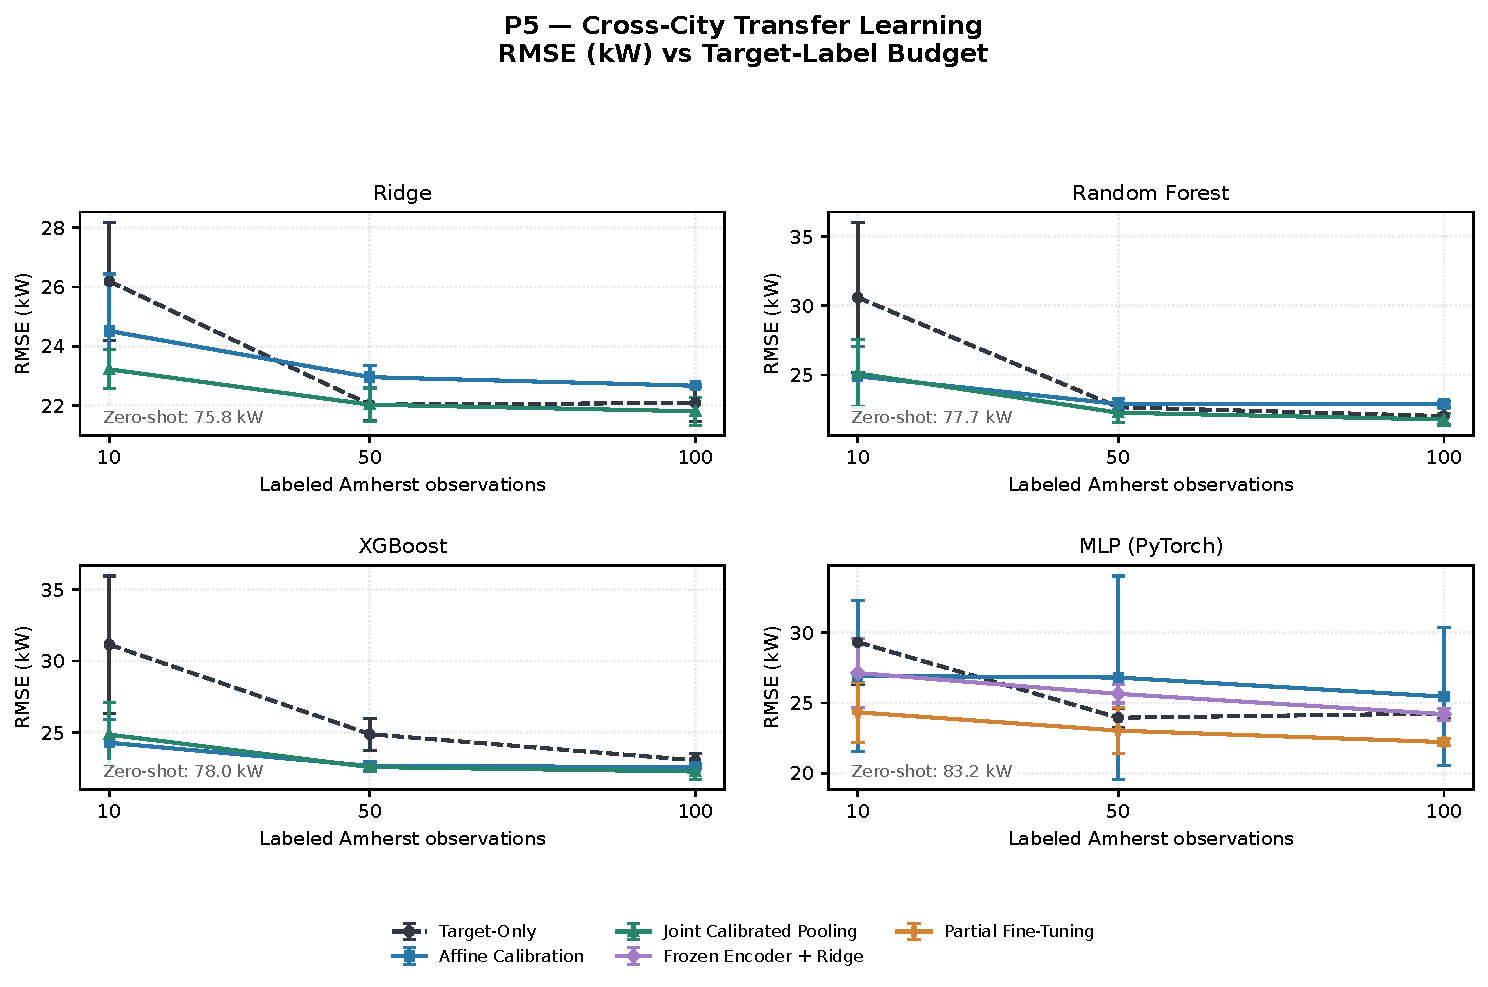
\includegraphics[width=0.94\textwidth]{Figures/P5/P5_RMSE_Label_Efficiency_All_Models.pdf}
\caption{Transfer-learning RMSE across target-label budgets, with the zero-shot level annotated in each panel.}\label{fig:p5rmsecurve}
\end{figure}
\begin{figure}[!htbp]\centering
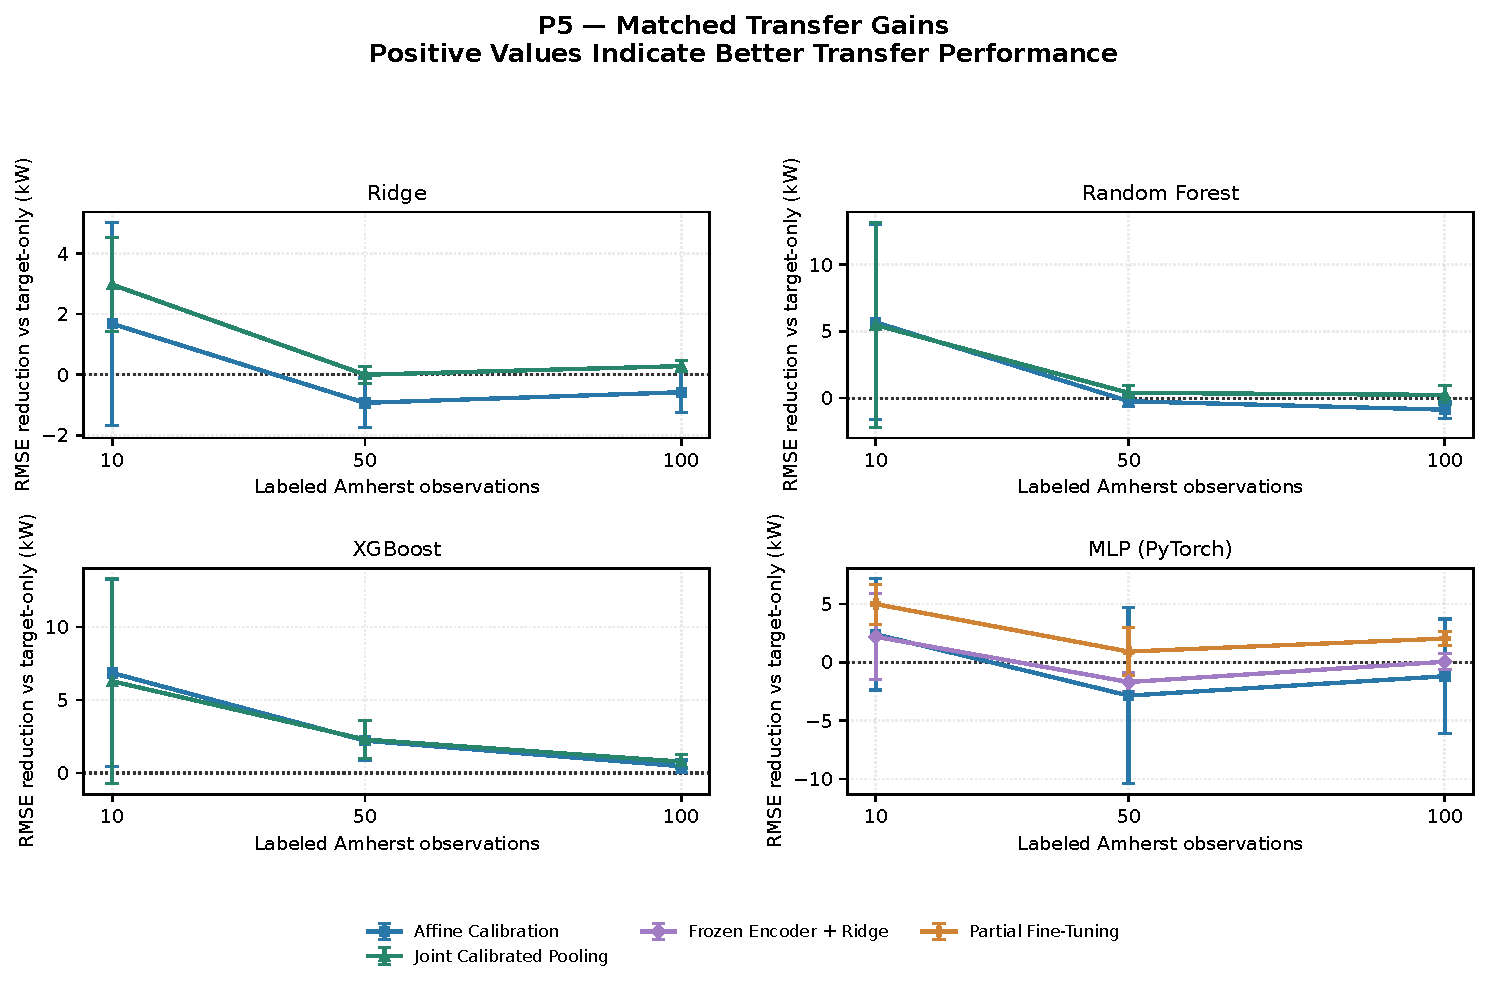
\includegraphics[width=0.90\textwidth]{Figures/P5/P5_RMSE_Transfer_Gains_All_Models.pdf}
\caption{Matched improvements (positive) or degradations (negative) relative to target-only training.}\label{fig:p5gaincurve}
\end{figure}

\subsection{Analysis: what transferred and what did not}
\paragraph{Both baselines are beaten.} At $k=10$, joint calibrated pooling with Ridge reaches
$23.22$\,kW, beating zero-shot ($75.82$\,kW, $-69\%$) and the best ten-label target-only model
($26.19$\,kW, $-11\%$). At $k=100$, pooling with random forest is again best ($21.80$ vs
$22.04$\,kW); at $k=50$ it ties the target-only Ridge.

\paragraph{What transferred: the shape of the weather-to-power relation.} Every method that keeps the
Davis model's \emph{relative} response and corrects only its level (affine calibration) or its
targets (pooling) works with ten labels. A two-parameter affine map removes most of the 75.8\,kW
zero-shot error, so most of that error was a scale and offset problem.

\paragraph{What did not transfer: absolute scale and site-specific effects.} Without target labels,
the Davis scale is carried over unchanged (P2). As $k$ grows, the target-only model learns
Amherst-specific effects that Davis cannot provide, and the advantage of transfer shrinks.

\paragraph{Robustness differs between strategies.} Joint pooling and partial fine-tuning never
produce negative transfer in Table~\ref{tab:p5matched}, whereas affine calibration hurts Ridge, RF
and the MLP once $k\ge50$: a global $a,b$ fitted on a few points cannot fix errors that vary across
conditions, while a model that has seen enough target data no longer needs it. Weak base learners
benefit most at $k=10$ (XGBoost $+6.85$\,kW, RF $+5.68$\,kW) because their target-only versions
overfit ten points badly (SD $\approx5$\,kW).
\FloatBarrier

% =================================================================
\section{Discussion}\label{sec:discussion}
\paragraph{One cause behind three results.} The Amherst Medium-regime errors (P1), the $>100\%$
zero-shot nRMSE (P2) and the large affine-calibration gain (P5) are three views of one fact: the
mapping from weather to power is site-specific, and its scale differs by a factor of about three
between Davis and the other sites. Models learn the weather side well; the power side has to be
re-anchored at each site.

\paragraph{Classical versus deep models.} Across P1--P5, tree ensembles (random forest, XGBoost)
are the most consistently strong models on this tabular data; the MLP ties them in Davis
regression and wins in Amherst regression, and the LSTM does not beat random forest on the
sequential task. Neural models help most where their representation can be reused or regularized:
the autoencoder in P3 at small $d$, autoencoder SSL for the MLP in P4, and partial fine-tuning in P5.

\paragraph{Failure modes observed.}
\begin{itemize}[leftmargin=1.5em,itemsep=2pt]
\item \textbf{Scale extrapolation:} every Davis-trained regressor over-predicts by roughly a factor of
three in unseen cities (P2).
\item \textbf{Boundary classes:} Partly Cloudy and Medium are the hardest classes everywhere (P1).
\item \textbf{Variance-maximizing compression:} PCA discards label-relevant directions for the sky task (P3).
\item \textbf{Confirmation bias in pseudo-labeling:} recycled errors lower logistic regression on Amherst generation (P4).
\item \textbf{Negative transfer:} affine calibration hurts three base models once $k\ge50$ (P5).
\item \textbf{Seed instability of neural models:} the MLP reaches SD $10.2$ BA points (P4) and $7.8$\,kW zero-shot (P5).
\end{itemize}

\paragraph{Limitations.}
(i) Cities differ in installed capacity and climate, and only five sites are available.
(ii) A finite set of hyperparameters and three seeds were evaluated; best test scores are
descriptive and slightly optimistic compared with strict validation-based selection.
(iii) Sky labels are derived from irradiance variables that the remaining predictors can partly
reconstruct: a physical proxy check reached about $99.8\%$ balanced accuracy in both tested
cities even with GHI and Clearsky GHI removed, so the very high sky scores reflect nowcasting from
correlated measurements.
(iv) The specification suggests normalizing per city in the cross-city protocol;
our zero-shot experiment reports the stricter raw-kW case. Normalizing the target per city (for
example, predicting power divided by a site capacity or by the training-city maximum) could address part of the power-scale bias, as suggested by the P5
calibration results.
(v) t-SNE and UMAP plots are qualitative.

% =================================================================
\section{Reproducibility}
\subsection{Protocol}
\begin{itemize}[leftmargin=1.5em,itemsep=2pt]
\item \textbf{Seeds:} $\{42,123,2026\}$ for every stochastic component (data subsampling, model
initialization, tree randomness, label masking in P4, target-sample selection in P5).
\item \textbf{Splits:} chronological 80/20 per sheet after timestamp sorting and removal of rows with
missing Output Power; the saved split indices are reused by every method in a comparison.
\item \textbf{Leakage control:} scalers, encoders, tercile thresholds, reducers and calibration maps
are fitted on training data (or on the $k$ target labels in P5) only.
\item \textbf{Reporting:} every metric is the mean $\pm$ SD over the three seeds.
\end{itemize}

\subsection{Environment and code}
Experiments were run in Python on Google Colab with scikit-learn~\cite{sklearn} (linear, kernel
and ensemble models, PCA, Nystr\"om, t-SNE), XGBoost~\cite{xgboost}, PyTorch~\cite{pytorch}
(MLP, LSTM, autoencoders) and \texttt{umap-learn}~\cite{umap}. The versions recorded by the
notebooks were Python~3.13.16, scikit-learn~1.6.1, XGBoost~3.4.1 and PyTorch~2.11.0 (CUDA~13.0),
on a Colab runtime with an NVIDIA Tesla~T4 GPU.

\paragraph{How to run.} The code, saved result tables and figures are available at
\url{https://github.com/myProjects400/ECE579-PV-ML-Project}. After installing
\texttt{requirements.txt}, open the notebooks in \texttt{Code\_base\_v2/} and run them in order:
\texttt{00\_Data\_Preparation} (reads the workbook, writes the processed sheets and the
chronological 80/20 split files to \texttt{Data/Processed/Splits}), then \texttt{P1}--\texttt{P5}.
Each notebook writes its metrics to \texttt{Results/P\textit{n}} and its figures to
\texttt{Figures/P\textit{n}}; the P4 label masks and P5 few-shot target samples are saved under
\texttt{Results/P4/Label\_Splits} and \texttt{Results/P5/Few\_Shot\_Splits}.

\subsection{AI assistance disclosure}
As permitted by the course policy, ChatGPT was used to help understand
library APIs, debug code and improve the wording of this report. All experiments were run by the
author, and all reported numbers come from those runs.

% =================================================================
\section{Conclusion}
This project compared five machine-learning paradigms for PV prediction on a common, leakage-safe
protocol. Same-city supervised models are accurate (sky BA up to $99.15\%$; power RMSE $11.85$\,kW,
$4.72\%$ nRMSE in Davis), but their accuracy does not survive a change of site: Davis-trained
regressors exceed $100\%$ nRMSE elsewhere, consistent with the large cross-city differences
in output-power scale and input distributions.
Unsupervised compression to ten or fewer dimensions always costs some accuracy, most for the sky
task whose label is a narrow irradiance ratio. Unlabeled data adds at most a few tenths of a point
for strong learners but stabilizes data-hungry neural models. The most practical result is that
very few target labels are enough to re-anchor a source model: ten Amherst observations with joint
calibrated pooling reduce RMSE by $69\%$ relative to zero-shot and beat the matched target-only model.



\clearpage
\appendix
\section{Supplementary P3 Regression MAE Results}\label{app:p3mae}
\noindent Table~\ref{tab:p3fullmae} completes the regression evaluation with the MAE of
all five downstream models at $d\in\{2,5,10\}$, using PCA, approximate RBF kernel PCA,
and autoencoder representations. The matched \emph{raw} column always refers to the same
regression model trained on original features. Results are held-out means $\pm$ standard
deviations over the three seeds.

{\footnotesize\setlength{\tabcolsep}{2.7pt}\renewcommand{\arraystretch}{1.10}
\begin{longtable}{@{}llp{2.35cm}rrrr@{}}
\caption{P3 held-out regression MAE (kW): original versus reduced features, matched by city and model (mean $\pm$ SD, three seeds).}\label{tab:p3fullmae}\\
\toprule
\textbf{City}&$d$&\textbf{Regressor}&\textbf{Raw}&\textbf{PCA}&\textbf{KPCA}&\textbf{AE}\\\midrule
\endfirsthead
\multicolumn{7}{l}{\footnotesize Table \thetable\ (continued)}\\
\toprule\textbf{City}&$d$&\textbf{Regressor}&\textbf{Raw}&\textbf{PCA}&\textbf{KPCA}&\textbf{AE}\\\midrule
\endhead
Davis & 2 & Ridge & 9.77\,$\pm$\,0.00 & 21.12\,$\pm$\,0.00 & 24.85\,$\pm$\,0.00 & 29.28\,$\pm$\,4.57 \\
Davis & 2 & RBF SVR & 11.43\,$\pm$\,0.00 & 16.54\,$\pm$\,0.00 & 19.73\,$\pm$\,0.00 & 17.72\,$\pm$\,2.37 \\
Davis & 2 & Random forest & 7.88\,$\pm$\,0.02 & 17.28\,$\pm$\,0.02 & 20.51\,$\pm$\,0.04 & 16.75\,$\pm$\,1.20 \\
Davis & 2 & XGBoost & 8.17\,$\pm$\,0.06 & 19.56\,$\pm$\,0.00 & 23.08\,$\pm$\,0.01 & 21.22\,$\pm$\,4.14 \\
Davis & 2 & MLP (PyTorch) & 8.71\,$\pm$\,0.18 & 16.79\,$\pm$\,0.22 & 19.41\,$\pm$\,0.21 & 16.53\,$\pm$\,1.51 \\
\addlinespace[2pt]
Davis & 5 & Ridge & 9.77\,$\pm$\,0.00 & 18.02\,$\pm$\,0.00 & 19.43\,$\pm$\,0.00 & 20.02\,$\pm$\,1.58 \\
Davis & 5 & RBF SVR & 11.43\,$\pm$\,0.00 & 12.44\,$\pm$\,0.00 & 13.00\,$\pm$\,0.00 & 11.54\,$\pm$\,0.87 \\
Davis & 5 & Random forest & 7.88\,$\pm$\,0.02 & 12.65\,$\pm$\,0.02 & 12.95\,$\pm$\,0.03 & 12.34\,$\pm$\,0.69 \\
Davis & 5 & XGBoost & 8.17\,$\pm$\,0.06 & 12.96\,$\pm$\,0.03 & 13.21\,$\pm$\,0.03 & 13.02\,$\pm$\,0.42 \\
Davis & 5 & MLP (PyTorch) & 8.71\,$\pm$\,0.18 & 12.73\,$\pm$\,0.22 & 13.03\,$\pm$\,0.26 & 11.82\,$\pm$\,0.51 \\
\addlinespace[2pt]
Davis & 10 & Ridge & 9.77\,$\pm$\,0.00 & 18.43\,$\pm$\,0.00 & 20.68\,$\pm$\,0.00 & 17.23\,$\pm$\,1.54 \\
Davis & 10 & RBF SVR & 11.43\,$\pm$\,0.00 & 18.51\,$\pm$\,0.00 & 16.64\,$\pm$\,0.00 & 11.20\,$\pm$\,0.27 \\
Davis & 10 & Random forest & 7.88\,$\pm$\,0.02 & 12.42\,$\pm$\,0.01 & 13.38\,$\pm$\,0.04 & 14.02\,$\pm$\,0.44 \\
Davis & 10 & XGBoost & 8.17\,$\pm$\,0.06 & 13.72\,$\pm$\,0.07 & 13.41\,$\pm$\,0.11 & 14.93\,$\pm$\,0.93 \\
Davis & 10 & MLP (PyTorch) & 8.71\,$\pm$\,0.18 & 12.46\,$\pm$\,0.40 & 13.84\,$\pm$\,0.50 & 11.42\,$\pm$\,0.55 \\
\addlinespace[2pt]
Amherst & 2 & Ridge & 14.61\,$\pm$\,0.00 & 20.07\,$\pm$\,0.00 & 18.14\,$\pm$\,0.00 & 27.50\,$\pm$\,4.02 \\
Amherst & 2 & RBF SVR & 20.71\,$\pm$\,0.00 & 19.21\,$\pm$\,0.00 & 17.42\,$\pm$\,0.00 & 19.07\,$\pm$\,2.02 \\
Amherst & 2 & Random forest & 13.56\,$\pm$\,0.04 & 20.36\,$\pm$\,0.02 & 18.39\,$\pm$\,0.06 & 19.30\,$\pm$\,1.92 \\
Amherst & 2 & XGBoost & 13.50\,$\pm$\,0.07 & 20.18\,$\pm$\,0.01 & 18.44\,$\pm$\,0.02 & 19.98\,$\pm$\,1.67 \\
Amherst & 2 & MLP (PyTorch) & 14.53\,$\pm$\,0.07 & 19.37\,$\pm$\,0.02 & 17.66\,$\pm$\,0.04 & 18.93\,$\pm$\,2.14 \\
\addlinespace[2pt]
Amherst & 5 & Ridge & 14.61\,$\pm$\,0.00 & 15.54\,$\pm$\,0.00 & 16.07\,$\pm$\,0.00 & 15.98\,$\pm$\,0.26 \\
Amherst & 5 & RBF SVR & 20.71\,$\pm$\,0.00 & 14.42\,$\pm$\,0.00 & 14.43\,$\pm$\,0.00 & 14.15\,$\pm$\,0.30 \\
Amherst & 5 & Random forest & 13.56\,$\pm$\,0.04 & 15.25\,$\pm$\,0.08 & 14.73\,$\pm$\,0.04 & 14.74\,$\pm$\,0.45 \\
Amherst & 5 & XGBoost & 13.50\,$\pm$\,0.07 & 14.50\,$\pm$\,0.11 & 14.83\,$\pm$\,0.07 & 14.38\,$\pm$\,0.20 \\
Amherst & 5 & MLP (PyTorch) & 14.53\,$\pm$\,0.07 & 14.39\,$\pm$\,0.17 & 14.38\,$\pm$\,0.07 & 14.58\,$\pm$\,0.28 \\
\addlinespace[2pt]
Amherst & 10 & Ridge & 14.61\,$\pm$\,0.00 & 15.49\,$\pm$\,0.00 & 15.24\,$\pm$\,0.00 & 15.38\,$\pm$\,0.46 \\
Amherst & 10 & RBF SVR & 20.71\,$\pm$\,0.00 & 16.28\,$\pm$\,0.00 & 14.83\,$\pm$\,0.00 & 14.38\,$\pm$\,0.63 \\
Amherst & 10 & Random forest & 13.56\,$\pm$\,0.04 & 15.37\,$\pm$\,0.09 & 14.91\,$\pm$\,0.01 & 15.23\,$\pm$\,0.33 \\
Amherst & 10 & XGBoost & 13.50\,$\pm$\,0.07 & 14.66\,$\pm$\,0.03 & 14.58\,$\pm$\,0.03 & 14.59\,$\pm$\,0.36 \\
Amherst & 10 & MLP (PyTorch) & 14.53\,$\pm$\,0.07 & 14.44\,$\pm$\,0.09 & 14.68\,$\pm$\,0.18 & 14.40\,$\pm$\,0.37 \\
\addlinespace[2pt]
\bottomrule\end{longtable}
}
\clearpage

% =================================================================
\begin{thebibliography}{9}
\bibitem{sklearn} scikit-learn: Machine Learning in Python. \url{https://scikit-learn.org}
\bibitem{xgboost} XGBoost: Scalable and Flexible Gradient Boosting. \url{https://xgboost.ai}
\bibitem{pytorch} PyTorch. \url{https://pytorch.org}
\bibitem{umap} UMAP: Uniform Manifold Approximation and Projection (\texttt{umap-learn}). \url{https://umap-learn.readthedocs.io}
\end{thebibliography}

\end{document}